\documentclass[11pt,a4paper]{report}
% ---------------------------------------------------------------------------
% Rapport : suivi de l'artificialisation des sols en Wallonie au regard du SDT 2024.
% Tous les chiffres proviennent de generated/chiffres.tex et generated/tab_*.tex,
% régénérés par `python src/construire_rapport.py`. Ne pas saisir de valeur à la main.
% ---------------------------------------------------------------------------
\usepackage[T1]{fontenc}
\usepackage[utf8]{inputenc}
\usepackage[french]{babel}
\usepackage{libertine}
\usepackage[libertine]{newtxmath}
\usepackage[a4paper,margin=2.4cm,headheight=14pt]{geometry}
\usepackage{microtype}
\usepackage{graphicx}
\usepackage{booktabs,makecell,longtable,multirow,array,threeparttable}
\usepackage{pdflscape}
\usepackage[table]{xcolor}
\usepackage{caption}
\usepackage{enumitem}
\usepackage{csquotes}
\usepackage{fancyhdr}
\usepackage{titlesec}
\usepackage[most]{tcolorbox}
\usepackage[numbers,sort&compress]{natbib}
\usepackage{xurl}
\usepackage[hidelinks]{hyperref}
\usepackage{bookmark}
\usepackage{float}
\urlstyle{same}
\addto\captionsfrench{\renewcommand{\tablename}{Tableau}}

% Généré par src/artif/rapport.py -- ne pas éditer
\newcommand{\AnneeDebutObs}{2021}
\newcommand{\AnneeFinObs}{2024}
\newcommand{\NbAnneesObs}{4}
\newcommand{\AnneeStock}{2025}
\newcommand{\RefDebut}{2010}
\newcommand{\RefFin}{2019}
\newcommand{\TrajDebut}{2021}
\newcommand{\TrajFin}{2050}
\newcommand{\NbCommunes}{261}
\newcommand{\NbCommunesSDT}{252}
\newcommand{\NbCommunesCG}{9}
\newcommand{\WalRef}{1\,160}
\newcommand{\WalRefKm}{11{,}6}
\newcommand{\WalRefRecalc}{1\,168}
\newcommand{\WalObsMoy}{1\,227}
\newcommand{\WalObsMoyKm}{12{,}3}
\newcommand{\WalCumObs}{4\,910}
\newcommand{\WalCumTraj}{4\,400}
\newcommand{\WalEcart}{510}
\newcommand{\WalRatio}{1{,}12}
\newcommand{\WalRatioRecalc}{1{,}11}
\newcommand{\WalPlafondFin}{1\,040}
\newcommand{\WalObsFin}{1\,374}
\newcommand{\WalBudget}{17\,399}
\newcommand{\WalBudgetKm}{174}
\newcommand{\WalBudgetConsommePct}{28}
\newcommand{\WalTrajQuinze}{999}
\newcommand{\WalTrajTrente}{801}
\newcommand{\WalVarPct}{+5{,}1}
\newcommand{\WalZ}{0{,}5}
\newcommand{\WalEcartType}{213}
\newcommand{\LuxVarPct}{+47}
\newcommand{\LuxZ}{7{,}3}
\newcommand{\NamVarPct}{+29}
\newcommand{\NamZ}{2{,}5}
\newcommand{\BWVarPct}{\textminus{}21}
\newcommand{\BWZ}{\textminus{}1{,}7}
\newcommand{\HDVarPct}{\textminus{}22}
\newcommand{\HDZ}{\textminus{}1{,}3}
\newcommand{\LuxRatio}{1{,}49}
\newcommand{\NamRatio}{1{,}48}
\newcommand{\LuxEcart}{324}
\newcommand{\NamEcart}{308}
\newcommand{\LuxNamPartEcart}{124}
\newcommand{\LuxObsMoy}{247}
\newcommand{\LuxRef}{175}
\newcommand{\NamObsMoy}{239}
\newcommand{\NamRef}{171}
\newcommand{\LuxRatioNeutre}{1{,}30}
\newcommand{\WalRatioNeutre}{1{,}08}
\newcommand{\NbBassinsAuDessus}{4}
\newcommand{\NbAuDessus}{144}
\newcommand{\NbDans}{107}
\newcommand{\NbNonInterp}{1}
\newcommand{\PartAuDessusPct}{57}
\newcommand{\RatioMed}{1{,}07}
\newcommand{\RatioQa}{0{,}77}
\newcommand{\RatioQc}{1{,}50}
\newcommand{\RatioMax}{9{,}3}
\newcommand{\CommuneRatioMax}{Tubize}
\newcommand{\RefCommuneRatioMax}{1{,}0}
\newcommand{\NbSautsSuivi}{12}
\newcommand{\NbSautsRef}{31}
\newcommand{\NbBasculeHaut}{6}
\newcommand{\NbBasculeBas}{6}
\newcommand{\NbAuDessusNeutre}{144}
\newcommand{\SensMin}{1{,}07}
\newcommand{\SensMax}{1{,}18}
\newcommand{\SensMinVar}{Définition « Principale + jardins et parcs + autres non bâties »}
\newcommand{\SensMaxVar}{Période de référence 2015-2019}
\newcommand{\SensNbVariantes}{14}
\newcommand{\SensComMin}{120}
\newcommand{\SensComMax}{151}
\newcommand{\PartArtifWal}{9{,}6}
\newcommand{\PartArtifWalLarge}{11{,}9}
\newcommand{\StockArtifKm}{1\,547}
\newcommand{\SautSeuil}{15}
\newcommand{\SautK}{6}
\newcommand{\ZeroMin}{2049{,}0}
\newcommand{\ZeroMax}{2049{,}0}
\newcommand{\IncertLecture}{2{,}2}
\newcommand{\NonCadRef}{627}
\newcommand{\NonCadObs}{37}
\newcommand{\MaisonsRef}{659}
\newcommand{\MaisonsObs}{522}
\newcommand{\ApptRef}{181}
\newcommand{\ApptObs}{335}
\newcommand{\AnnexesRef}{135}
\newcommand{\AnnexesObs}{196}
\newcommand{\AutresNBRef}{398}
\newcommand{\AutresNBObs}{337}
\newcommand{\BoisRef}{\textminus{}77}
\newcommand{\BoisObs}{\textminus{}212}
\newcommand{\PrincNonantePic}{22{,}9}
\newcommand{\PrincDixDix}{11{,}7}
\newcommand{\PythonVersion}{3.14.4}
\newcommand{\DateGeneration}{04/11/2026}
\newcommand{\WalDepassPct}{12}
\newcommand{\WalDepassFinPct}{32}
\newcommand{\WalBaisseAn}{40}
\newcommand{\WalEcartProj}{2\,500}
\newcommand{\PartTempsPct}{13}
\newcommand{\LUnRatio}{1{,}26}
\newcommand{\LUnRef}{70}
\newcommand{\HUnRatio}{0{,}93}
\newcommand{\HUnRatioRecalc}{1{,}10}
\newcommand{\HUnRef}{194}
\newcommand{\HUnRefRecalc}{165}
\newcommand{\SensCalageMin}{1{,}09}
\newcommand{\SensCalageMax}{1{,}16}
\newcommand{\SensDefLarge}{1{,}07}
\newcommand{\SensDefBati}{1{,}13}
\newcommand{\SensLectureDelta}{0{,}02}
\newcommand{\NbStatutsModifies}{12}
\newcommand{\NbVarHDDessous}{13}
\newcommand{\NbVarLUnDessus}{13}
\newcommand{\EcartFluxLarge}{3}
\newcommand{\PartAuDessusQuartBas}{75}
\newcommand{\PartAuDessusQuartHaut}{44}
\newcommand{\CorrPartRatio}{\textminus{}0{,}22}
\newcommand{\IwepsEcartRecent}{+1{,}0}
\newcommand{\IwepsEcartAncien}{+0{,}2}
\newcommand{\IwepsEcartQuatre}{+0{,}4}
\newcommand{\PrincDeuxMilleVingt}{1\,260}
\newcommand{\PrincVingtEtUnVingtTrois}{1\,179}
\newcommand{\CpdtEcartWal}{+17}
\newcommand{\CpdtEcartPct}{+1{,}5}
\newcommand{\CpdtEcartMin}{\textminus{}10}
\newcommand{\CpdtEcartMax}{+8}
\newcommand{\CpdtObsWal}{1\,162}
\newcommand{\CpdtRatioWal}{1{,}02}
\newcommand{\EtudeRatioTroisWal}{1{,}05}
\newcommand{\CpdtDepassPct}{2}
\newcommand{\EtudeDepassTroisPct}{5}
\newcommand{\CpdtRatioLux}{1{,}31}
\newcommand{\CpdtRatioNam}{1{,}33}
\newcommand{\CpdtRatioLUn}{0{,}83}
\newcommand{\CpdtRatioHUn}{1{,}01}
\newcommand{\LUnRefCpdt}{85}
\newcommand{\LUnRatioRefCpdt}{1{,}03}
\newcommand{\LUnRatioTrois}{1{,}00}
\newcommand{\LUnObsFin}{133}
\newcommand{\CpdtRefEcartAutres}{4}
\newcommand{\WalRatioRefCpdt}{1{,}10}
\newcommand{\WalRatioCal}{1{,}10}
\newcommand{\ArlonJ}{127}
\newcommand{\ArlonG}{108}
\newcommand{\BlegnyNC}{94}
\newcommand{\BlegnyRST}{94}
\newcommand{\BlegnyBati}{100}
\newcommand{\ValBatiStockQuinze}{8{,}3}
\newcommand{\ValBatiStockVingtTrois}{8{,}8}
\newcommand{\ValBatiFlux}{11{,}2}
\newcommand{\ValBatiFluxQuinze}{10{,}6}
\newcommand{\ValBatiCorr}{0{,}71}
\newcommand{\ValBatiCorrLag}{0{,}12}
\newcommand{\ValBatiMAE}{27}
\newcommand{\ValBatiEcartRef}{10}
\newcommand{\ValPrincStockQuinze}{8{,}7}
\newcommand{\ValPrincStockVingtTrois}{9{,}3}
\newcommand{\ValPrincFlux}{11{,}7}
\newcommand{\ValPrincFluxQuinze}{10{,}9}
\newcommand{\ValPrincCorr}{0{,}75}
\newcommand{\ValPrincCorrLag}{0{,}12}
\newcommand{\ValPrincMAE}{27}
\newcommand{\ValPrincEcartRef}{11}
\newcommand{\ValLargeStockQuinze}{11{,}1}
\newcommand{\ValLargeStockVingtTrois}{11{,}9}
\newcommand{\ValLargeFlux}{14{,}8}
\newcommand{\ValLargeFluxQuinze}{16{,}2}
\newcommand{\ValLargeCorr}{0{,}58}
\newcommand{\ValLargeCorrLag}{0{,}16}
\newcommand{\ValLargeMAE}{51}
\newcommand{\ValLargeEcartRef}{46}


% --- Couleurs (mêmes valeurs que les figures) -------------------------------
\definecolor{bleu}{HTML}{2a78d6}
\definecolor{orange}{HTML}{eb6834}
\definecolor{encre}{HTML}{0b0b0b}
\definecolor{encre2}{HTML}{52514e}
\definecolor{fond}{HTML}{f4f3ef}
\definecolor{fondbleu}{HTML}{eef5fd}

% --- Mise en page -------------------------------------------------------------
\setlength{\parskip}{0.45em}
\setlength{\parindent}{0pt}
\renewcommand{\arraystretch}{1.12}
\captionsetup{font=small,labelfont=bf,labelsep=period,justification=raggedright,singlelinecheck=false}
\setlist{itemsep=0.2em,topsep=0.3em}
\titleformat{\chapter}[hang]{\sffamily\bfseries\huge\color{encre}}{\thechapter}{0.8em}{}
\titlespacing*{\chapter}{0pt}{0pt}{1.5em}
\titleformat{\section}{\sffamily\bfseries\Large\color{encre}}{\thesection}{0.7em}{}
\titleformat{\subsection}{\sffamily\bfseries\large\color{encre}}{\thesubsection}{0.6em}{}
\titleformat{\paragraph}[runin]{\sffamily\bfseries\color{encre}}{}{}{}[.]
\pagestyle{fancy}
\fancyhf{}
\fancyhead[L]{\small\sffamily\color{encre2}Artificialisation des sols en Wallonie -- suivi du SDT 2024}
\fancyhead[R]{\small\sffamily\color{encre2}\leftmark}
\renewcommand{\chaptermark}[1]{\markboth{#1}{}}
\fancyfoot[C]{\small\sffamily\thepage}
\renewcommand{\headrulewidth}{0.3pt}
\fancypagestyle{plain}{\fancyhf{}\fancyfoot[C]{\small\sffamily\thepage}\renewcommand{\headrulewidth}{0pt}}

% --- Encadrés : choix méthodologiques, hypothèses, points d'attention ---------
\newtcolorbox{choix}[1]{enhanced,breakable,colback=fondbleu,colframe=bleu,boxrule=0pt,leftrule=2.5pt,
  arc=0pt,left=8pt,right=8pt,top=5pt,bottom=5pt,fonttitle=\sffamily\bfseries\small,coltitle=bleu,
  colbacktitle=fondbleu,attach title to upper,after title={\quad},title={#1}}
\newtcolorbox{attention}[1]{enhanced,breakable,colback=fond,colframe=orange,boxrule=0pt,leftrule=2.5pt,
  arc=0pt,left=8pt,right=8pt,top=5pt,bottom=5pt,fonttitle=\sffamily\bfseries\small,coltitle=orange!80!black,
  colbacktitle=fond,attach title to upper,after title={\quad},title={#1}}
\newtcolorbox{cle}{enhanced,breakable,colback=fond,colframe=fond,arc=0pt,left=10pt,right=10pt,top=8pt,bottom=8pt}

\newcommand{\fichier}[1]{\texttt{\small #1}}
\newcommand{\ha}{\,ha}
\newcommand{\haan}{\,ha/an}
\newcommand{\kmdan}{\,km²/an}

\hypersetup{pdftitle={Artificialisation des sols en Wallonie : suivi communal de la trajectoire du SDT 2024},
  pdfauthor={Étude indépendante}, pdflang={fr-BE}}

\begin{document}

% ============================================================================
\begin{titlepage}
\sffamily
\vspace*{1.5cm}
{\color{encre2}\large Étude indépendante -- note technique et méthodologique}\par
\vspace{1.2cm}
{\color{encre}\bfseries\fontsize{26}{31}\selectfont Artificialisation des sols en Wallonie\par}
\vspace{0.4cm}
{\color{encre}\Large Les bassins et les communes suivent-ils la trajectoire de réduction du Schéma de développement du territoire~2024~?\par}
\vspace{0.8cm}
{\color{bleu}\rule{\linewidth}{1.2pt}}\par
\vspace{0.4cm}
{\large Premier bilan \AnneeDebutObs--\AnneeFinObs{} à partir du registre cadastral (Statbel), méthode, validation, sensibilité et limites\par}
\vfill
\begin{tabular}{@{}ll}
\textbf{Version} & 1.0 -- données au 01/01/\AnneeStock{} \\
\textbf{Date} & \DateGeneration \\
\textbf{Auteur(s)} & [à compléter] \\
\textbf{Statut} & Document de travail, ouvert à la discussion \\
\textbf{Code et données} & chaîne reproductible \fichier{src/construire\_rapport.py} (annexe~\ref{ann:repro}) \\
\end{tabular}
\vspace{1cm}

{\small\color{encre2}Ce document est une analyse indépendante. Il n'émane ni du Gouvernement wallon, ni du SPW, ni de l'IWEPS, ni de la CPDT, et n'engage pas ces institutions. Les trajectoires du SDT y sont reconstituées à partir des graphiques publiés~; elles ne remplacent pas les valeurs officielles que l'administration pourrait publier. Les résultats communaux sont produits par une transposition analytique des règles du SDT, qui ne fixe pas de trajectoire par commune.\par}
\end{titlepage}

\pagenumbering{roman}
\tableofcontents
\clearpage
\pagenumbering{arabic}

% ============================================================================
\chapter*{Résumé exécutif}
\addcontentsline{toc}{chapter}{Résumé exécutif}
\markboth{Résumé exécutif}{}

\paragraph{Question} Le Schéma de développement du territoire (SDT), en vigueur depuis le 1\textsuperscript{er}~août~2024, fixe pour chacun des sept \enquote{bassins d'optimisation spatiale} wallons une trajectoire indicative de réduction de l'artificialisation nette~: partir de la moyenne des dix années précédant la pandémie et décroître linéairement jusqu'à 0\kmdan{} en 2050~\citep{sdt2024}. Cette étude vérifie, avec des données ouvertes et une chaîne de calcul entièrement scriptée, si la consommation observée depuis \AnneeDebutObs{} est compatible avec ces trajectoires, à l'échelle de la Wallonie, des bassins et des \NbCommunesSDT{} communes couvertes par le SDT.

\paragraph{Constats principaux}
\begin{enumerate}[leftmargin=1.4em]
\item \textbf{Wallonie : au-dessus de la trajectoire, de façon modérée.} De \AnneeDebutObs{} à \AnneeFinObs, \WalCumObs\ha{} ont été artificialisés (en net), contre \WalCumTraj\ha{} autorisés par la trajectoire (ratio \WalRatio, soit +\WalEcart\ha). La moyenne annuelle observée (\WalObsMoyKm\kmdan) dépasse la moyenne de référence du SDT (\WalRefKm\kmdan) au lieu de s'en écarter vers le bas. Sur \SensNbVariantes{} variantes de méthode, le ratio régional reste compris entre \SensMin{} et \SensMax~: le diagnostic \enquote{au-dessus} ne dépend d'aucun choix interne à l'étude. Il est confirmé par une source indépendante~: la note préparatoire au rapport triennal publiée par la CPDT en décembre 2025, calculée sur les données de l'IWEPS, place la Wallonie à \CpdtRatioWal{} de sa trajectoire sur 2021-2023~\citep{cpdt_prep2025}. Sur ces trois années, nos chiffres reproduisent ceux de la CPDT à \CpdtEcartPct\,\% près (ratio \EtudeRatioTroisWal). L'\emph{ampleur} du dépassement cumulé dépend donc fortement de l'année \AnneeFinObs{} (\WalObsFin\ha, la plus élevée de la période), que le cadastre peut encore réviser~: neutraliser les sauts cadastraux ramène le ratio à \WalRatioNeutre.
\item \textbf{Aucune décrue n'est encore visible.} La moyenne \AnneeDebutObs--\AnneeFinObs{} est statistiquement indiscernable de celle de \RefDebut--\RefFin{} ($z = \WalZ$ ; variation \WalVarPct\,\%). Le rythme d'artificialisation s'est stabilisé autour de 12\kmdan{} depuis 2015, après une forte baisse depuis les années 1990 (pic de \PrincNonantePic\kmdan). En quatre années (\PartTempsPct\,\% de la période 2021-2050), \WalBudgetConsommePct\,\% du \enquote{budget} cumulé implicite de la trajectoire ont déjà été consommés.
\item \textbf{Un écart concentré dans deux bassins.} Luxembourg (ratio \LuxRatio, +\LuxEcart\ha) et Namur (ratio \NamRatio, +\NamEcart\ha) concentrent à eux seuls plus que la totalité du dépassement régional~; leur consommation a augmenté nettement par rapport à la référence (respectivement \LuxVarPct\,\% et \NamVarPct\,\%), au-delà de la variabilité interannuelle habituelle. La CPDT aboutit au même constat pour ces deux bassins (ratios \CpdtRatioLux{} et \CpdtRatioNam{} sur 2021-2023). Le Brabant wallon, le Hainaut~1 et le Hainaut~2 sont sous leur trajectoire, Liège~2 est à l'équilibre. Liège~1 apparaît au-dessus (ratio \LUnRatio), mais ce résultat tient à la référence~: le graphique du SDT donne \LUnRef\haan, la trajectoire tracée par la CPDT part d'environ \LUnRefCpdt\haan{}~; avec cette dernière, le ratio tombe à \LUnRatioRefCpdt.
\item \textbf{Communes : un signal à manier avec précaution.} En appliquant à chaque commune la règle du SDT (ce que le SDT ne fait pas lui-même), \NbAuDessus{} communes sur \NbCommunesSDT{} (\PartAuDessusPct\,\%) sont au-dessus de leur trajectoire théorique~; le ratio médian vaut \RatioMed{} (écart interquartile \RatioQa--\RatioQc). À cette échelle, la série cadastrale est bruitée~: \NbSautsSuivi{} communes présentent depuis 2021 des sauts qui ressemblent davantage à des reclassements administratifs qu'à de l'artificialisation réelle, et doivent être vérifiées avant toute interprétation.
\item \textbf{La composition change.} La construction de maisons recule (\MaisonsRef{} $\rightarrow$ \MaisonsObs\haan), celle d'appartements progresse fortement (\ApptRef{} $\rightarrow$ \ApptObs\haan). La densification est donc engagée dans la production de logements, mais elle ne se traduit pas encore par une baisse de la surface consommée.
\end{enumerate}

\paragraph{Portée et limites} Le bilan porte sur \NbAnneesObs{} années, dont l'essentiel précède l'entrée en vigueur du SDT~; l'enregistrement cadastral d'un bâtiment suit son achèvement, souvent plusieurs années après le permis. Ce document constitue donc un \textbf{point zéro} plutôt qu'une évaluation des effets du SDT. Les trajectoires officielles n'étant publiées que sous forme de graphiques, elles ont été numérisées (incertitude de lecture de l'ordre de $\pm$\IncertLecture\haan{} par bassin). La définition cadastrale de l'artificialisation retenue ici reproduit les séries historiques du SDT (corrélation médiane \ValPrincCorr{} par bassin). Elle ne coïncide pas exactement avec celle de l'IWEPS, mais en reproduit les chiffres par bassin à \CpdtEcartMin{} à \CpdtEcartMax\haan{} près sur 2021-2023. Enfin, ce bilan s'arrête à \AnneeFinObs~: la fiche de l'IWEPS de septembre 2026 annonce un recul à 10,5\kmdan{} en 2025 pour l'ensemble de la Wallonie~\citep{iweps_t005}, année que cette étude n'intègre pas encore. Ce rythme est proche de la trajectoire de 2025~: il ferait baisser le ratio cumulé, sans résorber l'écart déjà accumulé. Cette lecture reste approximative, car elle mêle deux classifications et un périmètre différent.

\paragraph{Positionnement} Le CoDT impose un rapport triennal de suivi de l'artificialisation au regard du SDT~\citep{codt}. En décembre 2025, la CPDT en a publié une note préparatoire qui compare déjà, pour 2021-2023 et avec les données de l'IWEPS, l'artificialisation de chaque bassin à sa trajectoire~\citep{cpdt_prep2025,cpdt_monitoring2025}~; le premier rapport triennal officiel n'est pas encore publié. La présente étude n'est donc pas la première comparaison par bassin. Elle prolonge ce travail sur quatre points~: l'année \AnneeFinObs, un suivi communal à référence figée (l'outil ATOL-C de la CPDT offre déjà une vue communale, mais pour aider à élaborer les trajectoires~\citep{atolc2025}), une chaîne reproductible à partir de données ouvertes et une analyse systématique de la sensibilité des conclusions. Ses résultats par bassin convergent avec ceux de la CPDT, sauf pour Liège~1, en raison de la référence retenue (section~\ref{sec:cpdt}).

\paragraph{Recommandations principales} (i)~publier les valeurs chiffrées des trajectoires (le graphique du SDT et la note de la CPDT divergent pour Liège~1) et la série annuelle officielle par bassin prévue par la mesure SA1.M1~; (ii)~actualiser régulièrement la série communale ouverte de l'IWEPS (arrêtée au 1\textsuperscript{er}~janvier~2023 sur son API) et la publier en hectares~; (iii)~documenter les reclassements cadastraux majeurs~; (iv)~accélérer l'indicateur fondé sur les permis, seul capable de mesurer l'effet du SDT sans décalage~; (v)~croiser ces résultats avec une source d'observation de la Terre (WalOUS, Copernicus) pour suivre aussi l'imperméabilisation, que vise la nouvelle directive européenne sur les sols. Le détail figure au chapitre~\ref{ch:reco}.

% ============================================================================
\chapter{Introduction}
\label{ch:intro}

\section{Contexte et objet}
L'artificialisation des sols -- la transformation de terres agricoles, naturelles ou forestières en surfaces bâties, aménagées ou revêtues -- est devenue un objet de politique publique explicite en Europe depuis l'objectif indicatif de \enquote{zéro artificialisation nette} en 2050 formulé par la Commission en 2011~\citep{ce2011,ce2021}. En Wallonie, le SDT adopté le 23~avril~2024 traduit cet objectif en trajectoires chiffrées par bassin et prévoit leur suivi annuel~\citep{sdt2024}.

Cette étude poursuit trois objectifs~:
\begin{enumerate}[label=\textbf{O\arabic*}]
\item rendre explicites et réutilisables les trajectoires du SDT, qui ne sont publiées que sous forme graphique~;
\item construire, à partir de sources ouvertes et par une chaîne de traitement automatisée, un indicateur annuel d'artificialisation nette par commune et par bassin, validé contre les chiffres officiels~;
\item confronter la consommation observée depuis \AnneeDebutObs{} aux trajectoires, en documentant chaque choix, son effet sur les conclusions et les incertitudes qui demeurent.
\end{enumerate}

\section{Questions évaluatives}
\begin{description}[leftmargin=2.2em,style=nextline]
\item[Q1] Quelle trajectoire chaque bassin (et, par transposition, chaque commune) doit-il suivre, et avec quelle précision peut-on la connaître~?
\item[Q2] Quelles données permettent de mesurer l'artificialisation nette annuelle à l'échelle communale, et avec quelle fiabilité~?
\item[Q3] La consommation observée depuis \AnneeDebutObs{} est-elle compatible avec les trajectoires~?
\item[Q4] Ces conclusions résistent-elles aux choix méthodologiques raisonnables et à la variabilité des données~?
\end{description}

\section{Principes de l'étude}
\paragraph{Transparence} Chaque choix méthodologique est signalé dans un encadré bleu (\enquote{Choix C$n$}), chaque hypothèse non vérifiable dans un encadré orange (\enquote{Hypothèse H$n$}). Le registre complet figure au tableau~\ref{tab:registre}.
\paragraph{Reproductibilité} Aucun chiffre du rapport n'est saisi à la main~: tous sont produits par le code (\fichier{src/artif/}) à partir des sources téléchargées automatiquement, avec leur date d'accès et leur empreinte (annexe~\ref{ann:repro}).
\paragraph{Contestabilité} Les résultats sont accompagnés de leurs variantes. Un lecteur en désaccord avec un choix peut en mesurer l'effet (chapitre~\ref{ch:sens}) ou le modifier dans \fichier{src/artif/config.py} et relancer la chaîne.

% ============================================================================
\chapter{Cadre normatif}
\label{ch:cadre}

\section{Niveau européen}
L'objectif de \enquote{zéro artificialisation nette} (\emph{no net land take}) d'ici 2050 apparaît dans la feuille de route de 2011 pour une Europe efficace dans l'utilisation des ressources~\citep{ce2011} et est repris par la stratégie de l'UE pour les sols à l'horizon 2030~\citep{ce2021}. Il reste indicatif. La directive (UE) 2025/2360 du 12~novembre~2025 relative à la surveillance et à la résilience des sols~\citep{ue_sols2025} impose une surveillance de l'état des sols, de l'artificialisation et de l'imperméabilisation, dont les résultats doivent être rendus publics. Elle ne fixe pas d'objectif chiffré contraignant de zéro artificialisation nette, même si elle en rappelle l'horizon 2050. Elle doit être transposée d'ici décembre 2028. Ce texte rend pertinente, à moyen terme, une mesure de l'\emph{imperméabilisation} distincte de l'\emph{artificialisation} au sens cadastral utilisé ici (section~\ref{sec:limites}).

\section{Wallonie : le SDT 2024}
Le SDT, adopté par arrêté du Gouvernement wallon du 23~avril~2024 et entré en vigueur le 1\textsuperscript{er}~août~2024, remplace le SDER de 1999. Une version de 2019, qui prévoyait de réduire l'artificialisation à 6\kmdan{} en 2030, avait été retirée en 2022. Les dispositions pertinentes pour cette étude sont les suivantes~\citep{sdt2024}.

\begin{description}[leftmargin=1.2em,style=nextline]
\item[SA1.P1 -- Trajectoires de réduction de l'artificialisation (p.~40-42)] Pour chaque bassin d'optimisation spatiale, la trajectoire part de l'artificialisation nette moyenne des \enquote{dix dernières années, calculée avant la pandémie de COVID-19} et décroît vers 0\kmdan{} au plus tard en 2050. Pour la Wallonie hors Communauté germanophone, le texte cite une moyenne de 11,5\kmdan{} sur 2010-2020. Les trajectoires \enquote{servent de références dans le cadre d'un monitoring}~; elles sont présentées sous forme de graphiques, sans tableau de valeurs.
\item[SA1.M1 -- Monitoring] Un suivi annuel de l'artificialisation par bassin est prévu.
\item[SA1.P9 -- Compensation] Toute nouvelle artificialisation doit, à terme, être compensée, pour atteindre 0\kmdan{} net en 2050.
\item[SA1.M5 et SA2.M7 -- Échelle communale] Les communes doivent adopter, dans un délai de six ans, un schéma de développement communal (ou pluricommunal) \enquote{optimisation spatiale} comprenant leur propre trajectoire de réduction et l'objectif d'au moins trois logements neufs sur quatre en centralité en 2050.
\item[SA2.P2 -- Étalement résidentiel (p.~53-54)] Part des nouveaux logements localisés en centralité par bassin, avec un objectif de 75\,\% en 2050.
\item[Champ territorial] Les neuf communes de la Communauté germanophone, compétente en aménagement du territoire, sont exclues du SDT.
\end{description}

\begin{attention}{Statut juridique}
Le SDT a une valeur indicative. Ses trajectoires sont des références de suivi, non des plafonds opposables aux permis. Le SDT \emph{ne fixe pas} de trajectoire par commune~: les résultats communaux du chapitre~\ref{ch:resultats} appliquent par analogie la règle des bassins et n'ont pas de portée juridique.
\end{attention}

\paragraph{Bassins d'optimisation spatiale} Le SDT (p.~215) définit les bassins comme les territoires des directions extérieures du SPW Territoire~: Brabant wallon, Hainaut~1 (ouest), Hainaut~2 (est), Liège~1 (agglomération liégeoise), Liège~2 (reste de la province hors Communauté germanophone), Luxembourg et Namur.

\paragraph{Annexe CPDT de décembre 2025} La Conférence permanente du développement territorial a publié en décembre 2025 une annexe consacrée à la trajectoire d'artificialisation du foncier à vocation économique~\citep{cpdt2025}. Elle ne propose pas de trajectoire générale par bassin, mais apporte trois éléments utiles~: (i)~les terrains industriels et artisanaux sont passés de 16\,750\ha{} (2012) à 18\,113\ha{} (2024)~; (ii)~les besoins liés à la réindustrialisation sont estimés à 1\,343\ha{} d'ici 2035 et le potentiel de densification des parcs d'activité à 3\,516\ha~; (iii)~les permis devraient, à terme, devenir l'indicateur de référence, l'utilisation cadastrale du sol restant l'indicateur disponible dans l'intervalle.

\section{Travaux existants et positionnement de l'étude}
\label{sec:existant}
Une recherche documentaire menée en novembre 2026 a recensé les travaux suivants.

\paragraph{Indicateur régional de l'IWEPS} L'Institut wallon de l'évaluation, de la prospective et de la statistique produit l'indicateur de référence~\citep{iweps_t005,iweps_rs12}. Sa méthode est la suivante.
\begin{itemize}
\item \textbf{Source}~: la matrice cadastrale du SPF Finances (AGDP), situation au 1\textsuperscript{er}~janvier de chaque année. C'est la même source administrative que les statistiques de Statbel utilisées ici, mais à un niveau de détail plus fin.
\item \textbf{Classement}~: chaque parcelle porte une nature cadastrale (environ 250 natures). La nomenclature \enquote{CPDT-IWEPS-SPW Environnement} les regroupe en 16 catégories d'utilisation du sol, en tenant compte aussi du nombre de logements par parcelle. Neuf catégories sont artificialisées (résidentiel, commerces et services, équipements publics, loisirs et espaces verts urbains, bâtiments agricoles, industrie, carrières et décharges, transport, autres), six ne le sont pas, et une regroupe les terrains de nature inconnue, dont le non cadastré.
\item \textbf{Non cadastré}~: environ 5\,\% du territoire, surtout des voiries et des voies d'eau, n'a pas de nature cadastrale. Il est compté à part, hors des terrains artificialisés, d'où la fourchette de 11 à 16\,\% pour le taux d'artificialisation.
\item \textbf{Flux}~: l'artificialisation nette est la différence entre deux situations au 1\textsuperscript{er}~janvier, divisée par le nombre d'années. Elle est calculée par périodes de cinq ans pour la Wallonie et de trois ans pour les bassins~\citep{cpdt_monitoring2025}. Elle mesure un solde (terrains artificialisés moins terrains désartificialisés), et non des transferts entre catégories.
\item \textbf{Limites signalées par l'IWEPS}~: un changement de nature est attribué à toute la parcelle~; les mises à jour du cadastre peuvent être tardives~; la dernière année d'une matrice est incomplète.
\end{itemize}
Notre définition principale suit la même logique (parcelles bâties, terrains de loisirs et chemins cadastrés, non-cadastré exclu). Elle s'en écarte parce qu'elle repose sur les 27 rubriques agrégées de Statbel, alors que l'IWEPS classe les natures une à une. Le SPF Finances publie aussi ces natures par commune en données ouvertes~\citep{spf_occ}~; la présente étude ne les exploite pas encore. Le \emph{Regards statistiques} n\textsuperscript{o}~12~\citep{iweps_rs12} en tire les rythmes d'artificialisation nette les plus récents~: 12,2\kmdan{} entre 2010 et 2015, 10,8\kmdan{} sur 2015-2019 et 11,6\kmdan{} sur 2020-2022, soit une reprise à la hausse. La publication analyse l'étalement résidentiel par rapport aux centralités du SDT, mais ne confronte pas l'artificialisation aux trajectoires par bassin. La fiche T005 de septembre 2026~\citep{iweps_t005} actualise ces rythmes pour l'ensemble de la Wallonie~: 12,7\kmdan{} sur 2010-2014, 11,2 sur 2015-2019, 12,3 sur 2020-2024 et 10,5 pour la seule année 2025. Les données communales sont ouvertes (licence CC0)~: l'API de l'IWEPS~\citep{iweps_api} donne la part de chaque catégorie par commune, du 1\textsuperscript{er}~janvier~2002 au 1\textsuperscript{er}~janvier~2023 lors de notre consultation du 6~novembre~2026. Ces parts sont arrondies à 0,1\,point, soit environ 5\,ha pour une commune médiane~: c'est trop grossier pour mesurer un flux annuel communal.

\paragraph{Préparation du monitoring officiel} Le CoDT (art.~D.I.2, introduit par le décret du 13~décembre~2023) impose au Gouvernement un rapport triennal comprenant un \enquote{monitoring décrivant l'évolution de l'artificialisation, de l'étalement urbain et des disponibilités foncières, au regard des objectifs et orientations du schéma de développement du territoire}~\citep{codt}. Le Centre de ressources de la CPDT (Lepur-ULiège, en collaboration avec l'IWEPS) a été chargé d'en proposer la structure. Deux documents de décembre 2025 en rendent compte.
\begin{itemize}
\item La \textbf{note méthodologique}~\citep{cpdt_monitoring2025} retrace la sélection des indicateurs~: 27 proposés fin 2024, dont 22 \enquote{jugés prioritaires} après des réunions avec le comité technique au premier semestre 2025. Ils sont répartis en deux familles~: le suivi de l'\emph{action publique} (schémas communaux, révisions du plan de secteur, permis, sites à réaménager, opérations de développement urbain) et le suivi de l'\emph{impact territorial} (artificialisation, efficience, recentrage de l'urbanisation, disponibilités foncières). Les tableaux de la note détaillent 26 indicateurs, dont deux sont qualifiés d'optionnels~; l'écart avec le chiffre de 22 n'est pas expliqué. À la demande du comité technique, seuls les indicateurs d'impact ont été calculés. La note précise que les données nécessaires relèvent de l'administration régionale et que le suivi effectif dépendra de leur accessibilité. L'annexe~\ref{ann:indicateurs} détaille chaque indicateur, les données qu'il requiert et la difficulté de le produire.
\item La \textbf{note préparatoire} au rapport triennal~\citep{cpdt_prep2025} calcule ces indicateurs d'impact pour la Wallonie et ses sept bassins, à partir des données de l'IWEPS au 1\textsuperscript{er}~janvier~2024. Pour l'artificialisation, elle compare des moyennes par période de trois ans à la trajectoire de chaque bassin. Sur 2021-2023, elle conclut que le Brabant wallon, le Hainaut~2 et Liège~1 respectent leur trajectoire, que le Hainaut~1 et Liège~2 la respectent aussi \enquote{bien que les tendances récentes laissent entrevoir la nécessité d'efforts supplémentaires}, et que Namur et le Luxembourg s'en écartent. Elle estime l'artificialisation régionale à 11,6\kmdan{} sur 2020-2023, presque entièrement au détriment des terres agricoles. C'est, à notre connaissance, la première comparaison publiée aux trajectoires du SDT. La section~\ref{sec:cpdt} confronte nos résultats aux siens.
\end{itemize}
La recherche R1 de la CPDT traite par ailleurs de la trajectoire du seul foncier économique~\citep{cpdt2025}.

\paragraph{Recherche universitaire} Les travaux du Lepur (ULiège) analysent les conditions politiques et foncières du \enquote{zéro artificialisation nette}, en particulier le surdimensionnement des zones d'habitat et la question de l'indemnisation des déclassements~\citep{halleux2025}.

\paragraph{Flandre} L'administration (Departement Omgeving) cartographie la prise d'espace (\emph{ruimtebeslag}) tous les trois ans et l'imperméabilisation (\emph{verharding}) chaque année. Les deux indicateurs sont aussi publiés par commune~\citep{vlaanderen_landgebruik2025}. Deux travaux non gouvernementaux s'en servent pour évaluer les communes. Le \emph{Betonrapport 2024} de Natuurpunt et Breekijzer, réalisé avec HOGent, analyse l'évolution de l'imperméabilisation de 2013 à 2021 dans chaque commune~\citep{betonrapport2024}. La \emph{Betonmeter} de HOGent~\citep{betonmeter2025} répartit en outre l'objectif flamand entre les 300 communes (section~\ref{sec:regions})~: c'est l'équivalent le plus proche, en Flandre, de l'analyse communale de la présente étude.

\paragraph{Outil ATOL-C} Le CREAT-UCLouvain a développé pour la CPDT un outil web interactif d'aide à l'élaboration des trajectoires communales~\citep{atolc2025}. Pour chaque commune, à partir notamment des données de l'IWEPS, il présente l'artificialisation nette (historique, tendance linéaire prolongée jusqu'en 2050, moyenne des dix dernières années et trajectoire \enquote{fictive} vers le zéro net), la part des logements produits dans et hors des centralités, et le potentiel foncier. Ses auteurs le décrivent comme un prototype d'aide à la réflexion, qui ne fournit pas de réponse unique. Ils annoncent une mise à jour annuelle et citent l'évolution vers un outil de suivi comme une perspective. Consultée le 6~novembre~2026, la version en ligne présente une série communale de consommation de 2002 à 2021 (situation IWEPS au 1\textsuperscript{er}~janvier~2022). Sa trajectoire part de la moyenne 2012-2022, et non de la référence 2010-2019 du SDT~; elle convient donc à la réflexion sur une trajectoire, mais pas à la vérification du respect du SDT. L'interface n'offre ni choix de la période, ni téléchargement des séries.

\paragraph{Apport de l'étude} Par rapport aux travaux de la CPDT, la présente étude apporte~: (i)~l'année \AnneeFinObs, publiée par Statbel en 2025~; (ii)~un diagnostic annuel par commune avec la référence figée 2010-2019 du SDT, et jusqu'en \AnneeFinObs, là où ATOL-C part de 2012-2022 pour aider à concevoir une trajectoire~; (iii)~une chaîne entièrement reproductible à partir de données ouvertes, avec des flux communaux en hectares~; (iv)~la mesure systématique de la sensibilité des conclusions aux choix de méthode. En revanche, elle ne couvre ni l'étalement urbain (part des logements en centralité), ni l'imperméabilisation, ni les disponibilités foncières, que la CPDT traite.

\section{Comparaison avec la Flandre et Bruxelles}
\label{sec:regions}
Les trois Régions sont compétentes en aménagement du territoire et ont chacune leur approche (tableau~\ref{tab:regions}).

\begin{table}[ht]
\centering\scriptsize
\caption{Objectifs et suivi de l'artificialisation dans les trois Régions belges (situation en novembre 2026).}
\label{tab:regions}
\begin{tabular}{>{\raggedright\arraybackslash}p{2.2cm}>{\raggedright\arraybackslash}p{4.2cm}>{\raggedright\arraybackslash}p{4.4cm}>{\raggedright\arraybackslash}p{3.9cm}}
\toprule
& Wallonie & Flandre & Bruxelles \\
\midrule
Document et statut & SDT, arrêté du 23/04/2024, valeur indicative~\citep{sdt2024} & Beleidsplan Ruimte Vlaanderen, vision stratégique du 20/07/2018~; objectif confirmé en 2025~\citep{vlaanderen_brv,vlaanderen_brv2025} & Stratégie \enquote{Good Soil}, adoptée en mai 2024~\citep{bruxelles_goodsoil} \\
Objectif final & 0\kmdan{} d'artificialisation nette en 2050 & 0\,ha/jour de prise d'espace supplémentaire en 2040 & \enquote{Évoluer vers \enquote{zéro artificialisation} des sols d'ici à 2050}, présenté comme une priorité \\
Étapes intermédiaires & Décroissance linéaire depuis la moyenne 2010-2020 (\WalTrajTrente\haan{} en 2030) & 3\,ha/jour en 2025 (contre 6\,ha/jour en 2015) & Aucune~: une étude doit fixer la trajectoire \\
Déclinaison locale & 7 bassins chiffrés par le SDT~; trajectoires communales à fixer dans les SDC & Aucune répartition officielle du quota de 11\,933\,ha (2022-2040)~; répartition proposée par HOGent~\citep{betonmeter2025} & -- \\
Indicateur & Artificialisation nette~: terrains cadastrés à usage artificialisé (IWEPS) & \emph{Ruimtebeslag}~: zones d'habitat, d'activité, de transport et de loisirs, jardins et parcs compris & Imperméabilisation (surfaces imperméables) \\
Source et fréquence & Cadastre (SPF Finances), annuel & Carte d'utilisation du sol (raster 10\,m), tous les 3 ans~; carte d'imperméabilisation annuelle & Orthophotos et images satellite (apprentissage profond) \\
Échelle publiée & Région, bassins~; communes (dernière année) & Région et communes & Région~; carte par quartier \\
Dernière valeur & 11,6\kmdan{} (2020-2023)~; 11 à 16\,\% du territoire~\citep{cpdt_prep2025} & 3,8\,ha/jour (2019-2025)~; 32,7\,\% du territoire en 2025~; 15,7\,\% imperméabilisé en 2024~\citep{vlaanderen_ruimtebeslag} & 53,2\,\% imperméabilisé en 2022~\citep{bruxelles_impermeabilite} \\
\bottomrule
\end{tabular}
\end{table}

\paragraph{Des horizons différents} La Flandre vise l'arrêt de la prise d'espace dix ans avant la Wallonie (2040 contre 2050) et s'est fixé un jalon intermédiaire de 3\,ha/jour en 2025. Le rythme mesuré, 3,8\,ha/jour sur 2019-2025, montre que ce jalon n'est pas atteint. Bruxelles, déjà imperméabilisée à plus de 50\,\%, n'a pas encore de trajectoire~: sa stratégie prévoit d'abord une étude.

\paragraph{Des indicateurs non comparables} Les chiffres des trois Régions ne peuvent pas être additionnés ni comparés directement.
\begin{itemize}
\item Le \emph{ruimtebeslag} flamand comprend les jardins, les parcs, les terrains de sport et toutes les infrastructures de transport. Il est mesuré sur une carte d'utilisation du sol qui croise plusieurs sources, dont le cadastre.
\item L'indicateur wallon ne porte que sur les terrains cadastrés~: les voiries non cadastrées (environ 5\,\% du territoire) en sont exclues. Les terrains de nature inconnue sont comptés à part, d'où la fourchette de 11 à 16\,\%.
\item L'indicateur bruxellois mesure une couverture physique (l'imperméabilisation), et non un usage.
\end{itemize}
En ordre de grandeur, 3,8\,ha/jour représentent environ 14\kmdan{} pour la Flandre, contre 11,6\kmdan{} (soit 3,2\,ha/jour) pour la Wallonie. Une part de l'écart tient à la différence de définition.

\paragraph{La déclinaison locale, point faible commun} Aucune des deux Régions dotées d'un objectif chiffré ne l'a réparti officiellement entre ses communes. La Wallonie s'arrête aux sept bassins et renvoie aux schémas communaux. En Flandre, HOGent constate qu'\enquote{il n'existe pas (encore) de répartition de ce quota par l'autorité flamande ni par les provinces} (notre traduction)~\citep{betonmeter2025}. Il propose un modèle de répartition simple dans lequel chaque commune réduit sa propre prise d'espace, sans compensation entre communes. L'analyse communale de la présente étude repose sur la même logique. L'extension de la chaîne à la Flandre et à Bruxelles est une piste (chapitre~\ref{ch:reco}).

% ============================================================================
\chapter{Données}
\label{ch:donnees}

\section{Sources disponibles et critères de choix}
Mesurer une trajectoire annuelle par commune exige une source (a)~couvrant au moins 2010-2019 et les années récentes, (b)~annuelle, (c)~désagrégée par commune, (d)~proche de la définition utilisée par le SDT et (e)~ouverte. Le tableau~\ref{tab:sources} confronte les sources identifiées à ces critères.

\begin{table}[ht]
\centering\small
\caption{Sources mobilisables pour le suivi de l'artificialisation en Wallonie.}
\label{tab:sources}
\begin{tabular}{p{3.6cm}p{2.1cm}p{1.6cm}p{2.0cm}p{5.4cm}}
\toprule
Source & Période & Pas & Échelle & Usage dans l'étude \\
\midrule
\textbf{Statbel -- occupation du sol selon le registre cadastral}~\citep{statbel_occ} & 1983-2025 & annuel & commune & \textbf{Source principale}~: 27 rubriques, superficies au 1\textsuperscript{er}~janvier, recodées aux communes actuelles \\
IWEPS / CPDT -- artificialisation (natures cadastrales reclassées)~\citep{iweps_artif} & 1985-2023 & annuel & commune & Référence de validation~; série communale ouverte en parts arrondies à 0,1\,point, jusqu'au 01/01/2023~\citep{iweps_api}~; ATOL-C en affiche les flux en hectares jusqu'en 2021~\citep{atolc2025} \\
SPF Finances -- occupation du sol par nature cadastrale~\citep{spf_occ} & 2011-2026 & annuel & commune, division, secteur statistique & Non utilisé à ce stade~: source la plus détaillée et la plus récente (01/01/2026, publiée en juillet 2026)~; piste principale d'amélioration \\
SDT 2024 -- séries par bassin~\citep{sdt2024} & 2002-2021 & annuel & bassin & Validation (séries numérisées) et trajectoires \\
WalOUS (SPW, UCLouvain)~\citep{walous} & 2018 et suiv. & pluriannuel & pixel / parcelle & Non utilisé~: trop peu de millésimes pour une référence 2010-2019~; piste de croisement \\
Copernicus HRL Imperviousness~\citep{copernicus_hrl} & 2006-2018 (triennal), puis annuel & 3 ans & 10-20\,m & Non utilisé~: mesure l'imperméabilisation, pas l'artificialisation~; piste \\
Permis d'urbanisme / statistiques de permis~\citep{bulletin_permis} & longue & mensuel & commune & Non utilisé~: pas de superficie de terrain consommée~; indicateur avancé à développer \\
\bottomrule
\end{tabular}
\end{table}

\begin{choix}{Choix C1 -- Source principale}
Le registre cadastral publié par Statbel offre la série ouverte la plus longue et prête à l'emploi~: toutes les années y sont recodées aux communes actuelles. Le jeu du SPF Finances, plus détaillé et plus récent, n'est disponible par fichier qu'à partir de 2011 d'après nos essais, ce qui couvre la référence 2010-2019 sauf le stock au 01/01/2010. C'est aussi la base des indicateurs de l'IWEPS et des graphiques du SDT, ce qui garantit une cohérence de principe avec la référence officielle.
\end{choix}

\section{Le registre cadastral : contenu et limites}
Le jeu de données Statbel (fichier SQLite, table \fichier{TF\_EAE\_LAND\_OCCUPTN\_MATRIX}) donne, pour chaque commune et chaque année (situation au 1\textsuperscript{er}~janvier), la superficie en hectares de 25 rubriques de parcelles cadastrées, des parcelles non normalisées et de la superficie non cadastrée (annexe~\ref{ann:nomenclature}). Statbel a recodé toutes les années aux 261 communes actuelles, y compris la fusion Bastogne-Bertogne (code 82039). Les millésimes 1992 et 2006 manquent~: la variation de l'intervalle est répartie uniformément sur les années concernées, ce qui n'affecte ni la période de référence ni la période de suivi.

Quatre caractéristiques du cadastre conditionnent l'interprétation~:
\begin{enumerate}[label=\alph*)]
\item \textbf{Usage déclaré, non couverture physique.} La rubrique décrit la nature fiscale de la parcelle. Une parcelle bâtie compte entièrement, jardin compris~; une prairie revêtue d'un parking peut rester classée en terre agricole jusqu'à sa mise à jour.
\item \textbf{Décalage temporel.} Une construction entre au cadastre à son achèvement ou à sa déclaration, souvent plusieurs années après le permis. Les flux 2021-2024 reflètent pour l'essentiel des décisions antérieures au SDT.
\item \textbf{Domaine non cadastré.} Les voiries et le domaine public (environ 5\,\% du territoire) ne sont pas décrits~; leur évolution n'est pas mesurée, comme dans l'indicateur IWEPS. Le stock artificialisé est donc un minimum.
\item \textbf{Reclassements administratifs.} Des changements de rubrique sans changement sur le terrain (bois reclassé en terrain récréatif, intégration de domaine non cadastré) créent des sauts ponctuels (section~\ref{sec:sauts}).
\end{enumerate}

\section{Correspondance communes -- bassins}
\label{sec:bassins}
La correspondance est obtenue par requête automatisée sur le service ArcGIS REST du SPW (couche des ressorts des fonctionnaires délégués, mise à jour du 09/09/2025)~\citep{spw_dirext}, puisque les bassins coïncident par définition avec ces ressorts. Le résultat compte \NbCommunes{} communes~: \NbCommunesSDT{} couvertes par le SDT et \NbCommunesCG{} de la Communauté germanophone, exclues. La même requête fournit les contours communaux simplifiés utilisés pour les cartes.

% ============================================================================
\chapter{Méthodologie}
\label{ch:methode}

\section{Chaîne de traitement}
La chaîne (\fichier{python src/construire\_rapport.py}) enchaîne cinq étapes~: (1)~correspondance communes-bassins (API SPW)~; (2)~téléchargement du SDT et numérisation de ses graphiques~; (3)~téléchargement du registre cadastral et calculs~; (4)~figures~; (5)~génération des chiffres et tableaux du présent document. Chaque téléchargement est journalisé (URL, date, taille, SHA-256) dans \fichier{data/raw/PROVENANCE.json}. L'ensemble s'exécute en moins d'une minute à partir du cache.

\section{Reconstitution des trajectoires du SDT}
\label{sec:numerisation}
Le SDT ne publie aucune valeur chiffrée de ses trajectoires~: elles n'existent que sous forme d'images matricielles insérées dans le PDF. Plutôt que de les lire à l'\oe il, nous les numérisons automatiquement (\fichier{src/artif/sdt.py})~:
\begin{itemize}
\item extraction des images des pages 40 à 42 (artificialisation) et 53-54 (logements en centralité)~;
\item calage vertical sur le quadrillage gris des axes (0 à 400\haan, axes homogénéisés entre bassins) et horizontal sur les étiquettes 2002 et 2050~;
\item lecture de la moyenne décennale (trait bleu horizontal, médiane sur 120 colonnes de pixels), de la trajectoire (tirets verts, ajustement linéaire) et de la série historique annuelle (trait gris, une lecture par année)~;
\item planche de contrôle superposant les valeurs lues aux graphiques sources (annexe~\ref{ann:sdt}, figure~\ref{fig:qa}).
\end{itemize}

\paragraph{Précision} Une erreur d'un pixel et demi correspond à $\pm$\IncertLecture\haan{} au plus. La somme des sept moyennes lues (\WalRef\haan) est à 1\,\% des 11,5\kmdan{} cités dans le texte du SDT, ce qui valide la lecture. L'ajustement des tirets verts atteint zéro en \ZeroMin{} pour tous les bassins~; nous interprétons cette valeur comme un artefact graphique (le dernier point tracé au début de l'année 2050) et retenons le zéro en 2050, avec une variante de sensibilité.

\begin{table}[ht]
\centering\small
\caption{Trajectoires du SDT 2024 reconstituées par numérisation des graphiques (ha/an, sauf mention). Plafonds annuels selon le choix C2~; budget~: somme des plafonds 2021-2050 (dérivation de l'étude)~; dernière colonne~: part des nouveaux logements en centralité, décennie 2010-2020 (SA2.P2).}
\label{tab:sdt}
\begin{tabular}{lrrrrrrrr}
\toprule
Bassin & \makecell{Moyenne\\décennale} & \makecell{Incert.\\lecture} & 2025 & 2030 & 2040 & \makecell{Budget\\2021-2050 (ha)} & \makecell{Zéro lu\\(année)} & \makecell{Logements en\\centralité (\%)} \\
\midrule
Hainaut 1 & 194 & 2{,}2 & 167 & 134 & 67 & 2\,905 & 2\,049{,}0 & 46 \\
Hainaut 2 & 144 & 2{,}2 & 124 & 99 & 50 & 2\,160 & 2\,049{,}0 & 58 \\
Brabant wallon & 166 & 2{,}2 & 143 & 115 & 57 & 2\,494 & 2\,049{,}0 & 60 \\
Namur & 171 & 2{,}2 & 147 & 118 & 59 & 2\,560 & 2\,049{,}0 & 39 \\
Luxembourg & 175 & 2{,}2 & 151 & 121 & 60 & 2\,627 & 2\,049{,}0 & 30 \\
Liège 1 & 70 & 2{,}2 & 60 & 48 & 24 & 1\,046 & 2\,049{,}0 & 69 \\
Liège 2 & 240 & 2{,}2 & 207 & 166 & 83 & 3\,607 & 2\,049{,}0 & 35 \\
\midrule
\textbf{Wallonie (hors CG)} & \textbf{1\,160} & & 999 & 801 & 400 & 17\,399 & &  \\
\bottomrule
\end{tabular}

\end{table}

\begin{choix}{Choix C2 -- Forme de la trajectoire}
Plafond annuel de l'année $N$~: $T(N) = R \times (2050 - N) / (2050 - 2021)$, où $R$ est la moyenne de référence. La trajectoire vaut $R$ en 2021 et 0 en 2050. Les graphiques montrent un départ entre 2020 et 2021~; les calages 2020-2050, 2020-2049 et 2022-2050 sont testés au chapitre~\ref{ch:sens}.
\end{choix}

\section{Définition opérationnelle de l'artificialisation}
\label{sec:definition}
Le SDT (déclaration environnementale) considère comme artificialisés les terrains portant une construction ou une installation fixe autorisée, quelle que soit leur fonction. L'IWEPS opérationnalise cette notion en reclassant les quelque 216 natures cadastrales détaillées~; Statbel n'en diffuse que 25 regroupements. Trois définitions ont été construites et confrontées aux références officielles~:
\begin{description}[leftmargin=1.2em,style=nextline]
\item[Bâti seul] toutes les parcelles bâties (rubriques 2*)~;
\item[Principale] bâti + terrains récréatifs (1J) + chemins cadastrés et places (1L)~;
\item[Large] principale + jardins et parcs (1DI) + autres parcelles non bâties (1MNOP~: terrains industriels, chantiers, voies ferrées, carrières, parkings, cimetières, terrains militaires, terrains à bâtir\dots).
\end{description}

\begin{choix}{Choix C3 -- Définition principale}
La définition \enquote{principale} est retenue parce qu'elle reproduit le mieux les \emph{flux} du SDT (meilleure corrélation et plus faible écart avec ses séries par bassin, section~\ref{sec:validation}), alors que le suivi d'une trajectoire porte sur des flux. La définition large reproduit mieux le \emph{stock} publié par l'IWEPS, mais surestime le flux d'environ \EcartFluxLarge\kmdan, parce que la rubrique 1MNOP mêle des terrains réellement artificialisés et des reclassements administratifs. Les deux autres définitions sont conservées en variantes.
\end{choix}

\section{Convention temporelle}
Le registre donne des stocks au 1\textsuperscript{er}~janvier. La consommation nette de l'année $N$ est définie par $C(N) = S(N+1) - S(N)$~: le stock au 01/01/\AnneeStock{} fournit la consommation de \AnneeFinObs. La période de suivi couvre donc \AnneeDebutObs--\AnneeFinObs{} (\NbAnneesObs{} années).

\begin{choix}{Choix C4 -- Attribution de l'année}
Avec cette convention, la corrélation avec les séries du SDT est de \ValPrincCorr{}~; avec un décalage d'un an, elle tombe à \ValPrincCorrLag. La convention retenue est donc celle du SDT lui-même.
\end{choix}

\section{Indicateur d'écart à la trajectoire}
Pour une entité (Wallonie, bassin, commune) de référence $R$, on compare la consommation \emph{cumulée} observée depuis 2021 au cumul autorisé~:
\[
\text{ratio} = \frac{\sum_{N=2021}^{\AnneeFinObs} C(N)}{\sum_{N=2021}^{\AnneeFinObs} T(N)}, \qquad \text{écart} = \sum C(N) - \sum T(N)\ \text{(ha)}.
\]
Un ratio supérieur à 1 signifie \enquote{au-dessus de la trajectoire}. Le cumul est préféré à la comparaison de la seule dernière année, très sensible aux fluctuations annuelles, et correspond à la logique d'un budget. Le \enquote{budget} total 2021-2050 implicite de la trajectoire vaut environ $15\,R$ (\WalBudget\ha{} pour la Wallonie)~; c'est une dérivation de cette étude, non un chiffre du SDT.

\begin{choix}{Choix C5 -- Référence des bassins}
Pour les bassins, la référence est la moyenne lue sur les graphiques du SDT (référence officielle). La moyenne 2010-2019 recalculée à partir du cadastre est présentée en parallèle~; les deux diffèrent de \ValPrincEcartRef\haan{} en moyenne (en valeur absolue) par bassin.
\end{choix}

\section{Transposition aux communes}
\begin{choix}{Choix C6 -- Trajectoires communales théoriques}
Faute de trajectoire communale officielle, on applique à chaque commune la règle du SDT~: référence = moyenne communale 2010-2019 du cadastre, décroissance linéaire jusqu'à 0 en 2050. Une référence nulle ou négative rend le ratio non interprétable. Ce choix est purement analytique~: les communes définiront leur propre trajectoire dans leur schéma de développement communal, et pourront légitimement s'écarter de cette règle (centralités à renforcer, rattrapage de besoins en logement, etc.).
\end{choix}

\begin{attention}{Hypothèse H1 -- Équité de la règle uniforme}
La transposition suppose implicitement que chaque commune doit réduire sa consommation dans la même proportion. Or le SDT organise la réduction par bassin et entend concentrer le développement dans les centralités~: une commune-pôle peut être appelée à dépasser sa trajectoire théorique, une commune rurale à faire mieux. Le statut communal doit être lu comme un signal descriptif, non comme un jugement de conformité.
\end{attention}

\section{Détection des sauts cadastraux}
\label{sec:methode_sauts}
Une année est signalée \enquote{à vérifier} lorsque l'écart de sa consommation à la médiane communale 2000-\AnneeFinObs{} dépasse le maximum de \SautSeuil\ha{} et de \SautK{} fois l'écart absolu médian (MAD) de la commune. Ce critère robuste repère les ruptures ponctuelles sans être influencé par elles.

\begin{choix}{Choix C7 -- Signaler plutôt que corriger}
Les sauts sont signalés et non corrigés dans l'indicateur principal~: certains correspondent à de vrais projets (zone d'activité, lotissement), d'autres à des reclassements. Seule une vérification parcellaire (AGDP, commune) permet de trancher. Une variante \enquote{sauts neutralisés} remplace chaque année signalée par la médiane communale.
\end{choix}

\section{Diagnostic statistique}
Pour distinguer une évolution réelle des fluctuations interannuelles, on calcule pour chaque bassin l'écart standardisé
\[
z = \frac{\bar C_{2021\text{-}\AnneeFinObs} - \bar C_{2010\text{-}2019}}{s\sqrt{1/10 + 1/\NbAnneesObs}},
\]
où $s$ est l'écart-type interannuel 2010-2019. Une valeur $|z| > 2$ indique un changement de niveau peu compatible avec la seule variabilité passée.

\begin{attention}{Hypothèse H2 -- Indépendance des années}
Le calcul de $z$ suppose les années indépendantes et la variance stable. L'autocorrélation (étalement des enregistrements cadastraux sur plusieurs années) rendrait le test trop optimiste~; il est présenté comme un indicateur d'ordre de grandeur, pas comme un test formel.
\end{attention}

% ============================================================================
\chapter{Validation de l'indicateur}
\label{sec:validation}

\begin{table}[ht]
\centering\footnotesize
\caption{Validation des trois définitions cadastrales contre les références officielles. Stock~: Wallonie entière~; flux et corrélations~: hors Communauté germanophone. $r$ médian et écart absolu~: comparaison annuelle aux séries des sept bassins du SDT (2002-2021). Références~: $^{a}$ IWEPS, 2021~; $^{b}$ SDT, 2010-2020~; $^{c}$ IWEPS, \emph{Regards statistiques} n\textsuperscript{o}~12, 2015-2019.}
\label{tab:validation}

\resizebox{\textwidth}{!}{\begin{tabular}{p{4.4cm}rrrrrrrr}
\toprule
Définition & \makecell{Stock\\2015 (\%)} & \makecell{Stock\\2023 (\%)} & \makecell{Flux 2010-19\\(km²/an)} & \makecell{Flux 2015-19\\(km²/an)} & \makecell{|Réf. bassin\\ $-$ SDT| (ha)} & \makecell{$r$ médian\\(même année)} & \makecell{Écart abs.\\moyen (ha)} & \makecell{$r$ médian\\(décalage 1 an)} \\
\midrule
Parcelles bâties seules & 8{,}3 & 8{,}8 & 11{,}2 & 10{,}6 & 10 & 0{,}71 & 27 & 0{,}12 \\
Bâti + terrains récréatifs + chemins cadastrés \textbf{(retenue)} & 8{,}7 & 9{,}3 & 11{,}7 & 10{,}9 & 11 & 0{,}75 & 27 & 0{,}12 \\
Principale + jardins et parcs + autres non bâties & 11{,}1 & 11{,}9 & 14{,}8 & 16{,}2 & 46 & 0{,}58 & 51 & 0{,}16 \\
\addlinespace \emph{Références publiées} & & $\geq$\,10{,}8$^{a}$ & 11{,}5$^{b}$ & 10{,}8$^{c}$ & & & & \\
\bottomrule
\end{tabular}
}
\end{table}

\paragraph{Niveau régional} La définition principale donne un flux moyen de \ValPrincFlux\kmdan{} sur 2010-2019 et de \ValPrincFluxQuinze\kmdan{} sur 2015-2019, à comparer aux 11,5\kmdan{} du SDT (2010-2020) et aux 10,8\kmdan{} de l'IWEPS (2015-2019)~\citep{iweps_rs12}. Son stock (\ValPrincStockVingtTrois\,\% en 2023) est en revanche inférieur à celui de l'IWEPS (10,9\,\%)~: la définition principale exclut une partie de la rubrique 1MNOP et des jardins que l'IWEPS compte. Pour le suivi de flux, cette sous-estimation de niveau est sans conséquence tant qu'elle est stable.

\paragraph{Comparaison aux rythmes publiés par l'IWEPS}
\label{sec:iweps}
Le tableau~\ref{tab:iweps} confronte nos trois définitions aux rythmes régionaux publiés par l'IWEPS pour la Wallonie francophone, dans deux millésimes successifs~: le \emph{Regards statistiques} n\textsuperscript{o}~12 (données au 1\textsuperscript{er}~janvier~2023)~\citep{iweps_rs12} et la note préparatoire de la CPDT (données au 1\textsuperscript{er}~janvier~2024)~\citep{cpdt_prep2025}. Les bornes des périodes sont interprétées en années de consommation (\enquote{entre 2010 et 2015} = consommations 2010 à 2014)~; la section~\ref{sec:cpdt} confirme cette lecture. Sur 2010-2019, la définition principale reproduit l'IWEPS à $\pm$\,0,2\kmdan{} près, ce qui conforte le choix C3. Sur 2020-2022, elle le dépasse de \IwepsEcartRecent\kmdan, mais l'écart tombe à \IwepsEcartQuatre\kmdan{} sur 2020-2023 avec le millésime suivant. Il se concentre sur 2020 (\PrincDeuxMilleVingt\ha{} dans notre série), qui comprend le reclassement de \BlegnyNC\ha{} de domaine non cadastré à Blegny (section~\ref{sec:sauts}). Il tient aussi probablement à la révision des années récentes d'un millésime à l'autre~: l'IWEPS signale que la dernière année d'une matrice cadastrale est incomplète~\citep{iweps_rs12}. L'année 2020 se situe hors de la période de suivi.

\begin{table}[ht]
\centering\small
\caption{Rythme annuel moyen d'artificialisation nette (km²/an), Wallonie hors Communauté germanophone~: IWEPS (deux millésimes) et définitions cadastrales de l'étude.}
\label{tab:iweps}
\begin{tabular}{lrlrrrr}
\toprule
\makecell{Années de\\consommation} & IWEPS & \makecell{Publication\\(millésime)} & Bâti seul & Principale & Large & \makecell{Écart\\principale $-$ IWEPS} \\
\midrule
2010-2014 & 12{,}2 & RS12 (2024) & 11{,}8 & \textbf{12{,}4} & 13{,}4 & +0{,}2 \\
2015-2019 & 10{,}8 & RS12 (2024) & 10{,}6 & \textbf{10{,}9} & 16{,}2 & +0{,}1 \\
2020-2022 & 11{,}6 & RS12 (2024) & 12{,}6 & \textbf{12{,}6} & 16{,}8 & +1{,}0 \\
2020-2023 & 11{,}6 & CPDT (2025) & 12{,}0 & \textbf{12{,}0} & 15{,}1 & +0{,}4 \\
\bottomrule
\end{tabular}

\end{table}

\paragraph{Comparaison par bassin à la note préparatoire de la CPDT}
\label{sec:cpdt}
La note préparatoire de la CPDT~\citep{cpdt_prep2025} représente, pour chaque bassin (fig.~17 à 23), deux éléments de nature différente~:
\begin{itemize}
\item des \textbf{barres}, qui sont des mesures~: l'artificialisation annuelle nette moyenne par période de trois ans, calculée par l'IWEPS selon la méthode décrite en section~\ref{sec:existant}~;
\item une \textbf{ligne}, qui est un objectif~: la trajectoire du SDT telle que la CPDT l'a tracée.
\end{itemize}
La comparaison des barres avec nos chiffres teste donc nos données contre celles de l'IWEPS, bassin par bassin. La ligne ne sert qu'à vérifier que nous lisons la même trajectoire que la CPDT. Les valeurs ne sont pas imprimées sur ces graphiques, mais ceux-ci sont vectoriels~: la chaîne télécharge le document, lit les coordonnées exactes des barres et des sommets de la trajectoire, et les convertit en ha/an par calage sur la grille (module \fichier{cpdt.py}, fichier \fichier{references/cpdt\_2025\_bassins.csv}). Il ne s'agit pas d'une lecture à l'\oe il d'une image~: un point typographique vaut environ 2\,ha, et les coordonnées sont connues au centième de point, si bien que l'erreur de lecture est négligeable devant les écarts observés. Les légendes des figures~20 et~21 sont interverties dans le document~; on retient le titre inscrit dans chaque graphique. Le tableau~\ref{tab:cpdt} confronte ces valeurs aux nôtres.

\begin{table}[ht]
\centering\footnotesize
\caption{Artificialisation annuelle nette par bassin (ha/an) et ratio à la trajectoire~: note préparatoire de la CPDT (données IWEPS au 01/01/2024) et présente étude (définition principale). $^{a}$ Référence implicite de la trajectoire tracée par la CPDT (pente $\times$ 29)~; $^{b}$ moyenne lue sur le graphique du SDT~; $^{c}$ moyenne 2021-2023 rapportée à la trajectoire du SDT au milieu de la période, comme le fait la CPDT.}
\label{tab:cpdt}
\resizebox{\textwidth}{!}{\begin{tabular}{lrrrrrrrr}
\toprule
Bassin & \makecell{CPDT/IWEPS\\2021-2023} & \makecell{Étude\\2021-2023} & Écart & \makecell{Réf.\\CPDT$^{a}$} & \makecell{Réf.\\SDT$^{b}$} & \makecell{Ratio CPDT\\2021-2023} & \makecell{Ratio étude\\2021-2023$^{c}$} & \makecell{Ratio étude\\2021-2024} \\
\midrule
Brabant wallon & 130 & 136 & +5 & 168 & 166 & \textbf{0{,}80} & 0{,}85 & 0{,}85 \\
Hainaut 1 & 186 & 176 & \textminus{}10 & 190 & 194 & \textbf{1{,}01} & 0{,}94 & 0{,}93 \\
Hainaut 2 & 102 & 107 & +5 & 143 & 144 & \textbf{0{,}74} & 0{,}77 & 0{,}89 \\
Liège 1 & 68 & 67 & \textminus{}1 & 85 & 70 & \textbf{0{,}83} & 1{,}00 & 1{,}26 \\
Liège 2 & 229 & 234 & +5 & 244 & 240 & \textbf{0{,}97} & 1{,}01 & 1{,}01 \\
Luxembourg & 222 & 226 & +4 & 176 & 175 & \textbf{1{,}31} & 1{,}34 & 1{,}49 \\
Namur & 224 & 232 & +8 & 175 & 171 & \textbf{1{,}33} & 1{,}41 & 1{,}48 \\
\midrule
\textbf{Wallonie (hors CG)} & 1\,162 & 1\,179 & +17 & 1\,181 & 1\,160 & \textbf{1{,}02} & 1{,}05 & 1{,}12 \\
\bottomrule
\end{tabular}
}
\end{table}

\begin{itemize}
\item \textbf{Les données concordent.} Sur 2021-2023, l'écart par bassin varie de \CpdtEcartMin{} à \CpdtEcartMax\haan{} et l'écart régional vaut \CpdtEcartWal\haan{} (\CpdtEcartPct\,\%). Décaler nos années d'un an dégrade nettement l'accord, ce qui confirme la convention C4. Sur les périodes antérieures, les écarts sont plus grands pour certains bassins (Hainaut~1 en 2009-2011, Namur en 2012-2014)~: les deux séries ne traitent pas tous les reclassements de la même manière.
\item \textbf{Les trajectoires concordent, sauf pour Liège~1.} Pour six bassins, la référence implicite de la CPDT diffère de moins de \CpdtRefEcartAutres\haan{} de celle que nous lisons sur le SDT. Pour Liège~1, la CPDT part d'environ \LUnRefCpdt\haan, contre \LUnRef\haan{} sur le graphique du SDT (vérifié visuellement, p.~42). La note ne précise pas comment ses trajectoires ont été établies. La valeur de \LUnRefCpdt\haan{} correspond à la moyenne de ses propres barres 2009-2020 pour ce bassin.
\item \textbf{Les diagnostics convergent sur 2021-2023.} Luxembourg et Namur sont au-dessus dans les deux études, le Brabant wallon et le Hainaut~2 en dessous, le Hainaut~1 et Liège~2 proches de l'équilibre. Pour Liège~1, la différence ne vient pas des données~: avec la référence du SDT, nos chiffres placent le bassin à l'équilibre (\LUnRatioTrois), alors que la CPDT le place en dessous (\CpdtRatioLUn). Sur 2021-2024, l'année \AnneeFinObs{} (\LUnObsFin\ha) porte notre ratio à \LUnRatio.
\item \textbf{L'année \AnneeFinObs{} pèse lourd.} Au niveau régional, le ratio passe de \CpdtRatioWal{} (CPDT) et \EtudeRatioTroisWal{} (étude) sur 2021-2023 à \WalRatio{} sur 2021-2024. Le dépassement régional que mesure l'étude repose donc en grande partie sur une seule année, la plus récente et la moins consolidée.
\end{itemize}

\paragraph{Niveau des bassins} La figure~\ref{fig:validation} confronte, année par année, la reconstitution cadastrale aux séries historiques du SDT. L'accord est bon pour la majorité des points~; les écarts importants concernent quelques années isolées où le SDT a vraisemblablement neutralisé des reclassements que le cadastre brut conserve. C'est un argument pour ne pas sur-interpréter une année communale isolée.

\begin{figure}[ht]
\centering
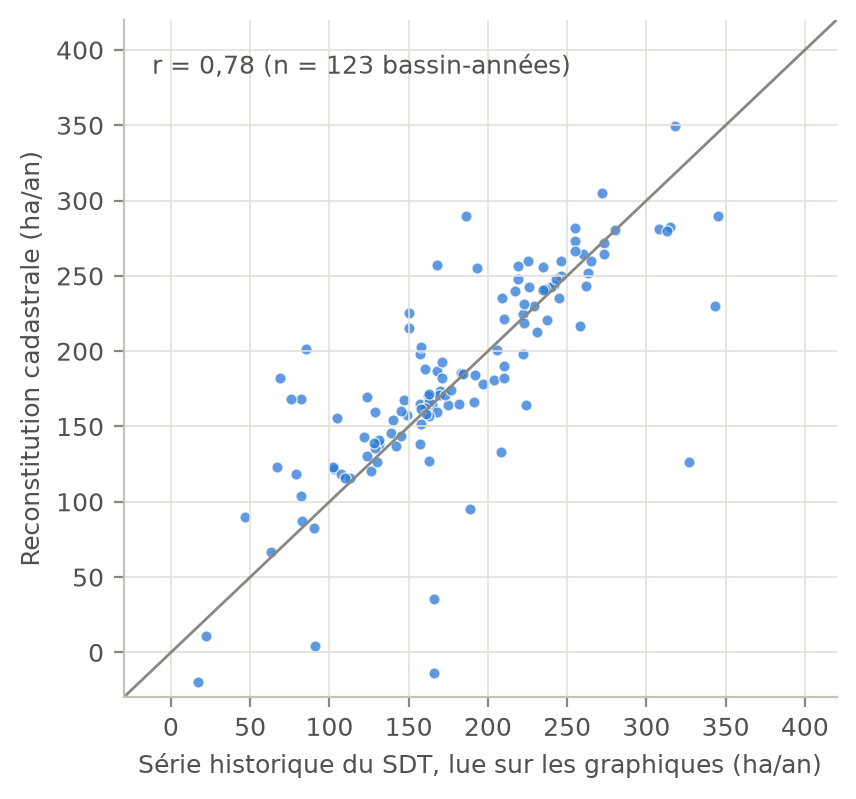
\includegraphics[width=0.56\textwidth]{figures/validation_scatter.png}
\caption{Consommation nette annuelle par bassin (2002-2021)~: série historique du SDT, lue sur ses graphiques, et reconstitution cadastrale (définition principale). La droite est la diagonale $y = x$.}
\label{fig:validation}
\end{figure}

\begin{figure}[ht]
\centering
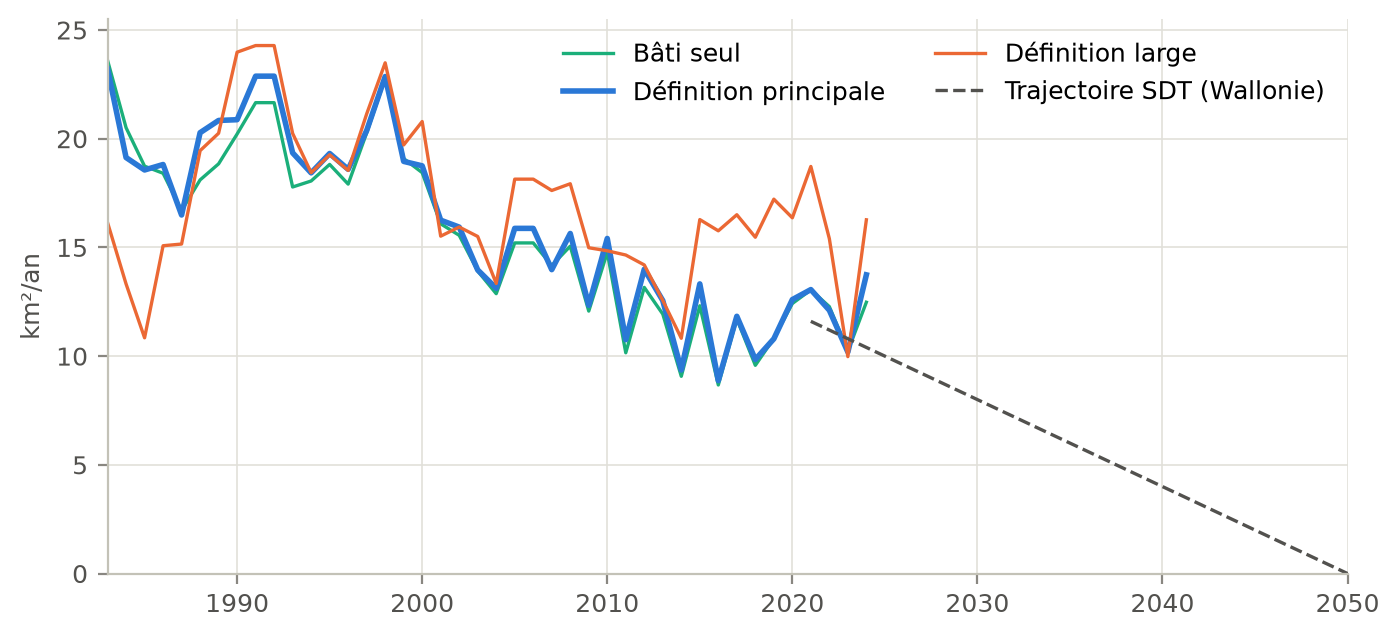
\includegraphics[width=0.92\textwidth]{figures/wallonie_long.png}
\caption{Consommation nette annuelle de la Wallonie hors Communauté germanophone, 1983-\AnneeFinObs, selon les trois définitions, et trajectoire du SDT.}
\label{fig:long}
\end{figure}

La figure~\ref{fig:long} replace la période étudiée dans la série longue~: la consommation a été divisée par deux depuis le début des années 1990, mais plafonne autour de 10-13\kmdan{} depuis 2014. La définition large diverge des deux autres à partir de 2005, signe de reclassements dans la rubrique 1MNOP.

% ============================================================================
\chapter{Résultats}
\label{ch:resultats}

\section{Wallonie}
\begin{cle}
\textbf{\WalCumObs\ha{} consommés de \AnneeDebutObs{} à \AnneeFinObs{}, pour \WalCumTraj\ha{} autorisés~: ratio \WalRatio, dépassement de \WalEcart\ha.}
En \AnneeFinObs, la consommation (\WalObsFin\ha) dépasse de \WalDepassFinPct\,\% le plafond annuel de la trajectoire (\WalPlafondFin\ha). Avec la référence recalculée (\WalRefRecalc\haan), le ratio vaut \WalRatioRecalc.
\end{cle}

Le dépassement est modeste en proportion, mais préoccupant dans sa dynamique~: la trajectoire exige une baisse d'environ \WalBaisseAn\haan{} chaque année, alors que la consommation observée ne baisse pas. La moyenne 2021-\AnneeFinObs{} (\WalObsMoy\haan) est même légèrement supérieure à la référence 2010-2019 recalculée, avec un écart ($z=\WalZ$) qui reste dans la variabilité habituelle (écart-type interannuel de \WalEcartType\haan). Le diagnostic le plus juste est donc~: \emph{pas de décrochage vers le bas, stabilité au niveau d'avant le SDT}.

\section{Bassins}
\begin{table}[ht]
\centering\footnotesize
\caption{Consommation nette annuelle observée et confrontation à la trajectoire par bassin (ha). Ratio (SDT)~: référence lue sur les graphiques du SDT (indicateur principal)~; ratio (recalc.)~: référence 2010-2019 recalculée sur le cadastre.}
\label{tab:bassins}

\resizebox{\textwidth}{!}{\begin{tabular}{lrrrrrrrrrrr}
\toprule
Bassin & \makecell{Réf.\\SDT} & \makecell{Réf.\\recalc.} & 2021 & 2022 & 2023 & 2024 & \makecell{Cumul\\observé} & \makecell{Cumul\\autorisé} & Écart & \makecell{Ratio\\(SDT)} & \makecell{Ratio\\(recalc.)} \\
\midrule
Brabant wallon & 166 & 171 & 122 & 128 & 157 & 129 & 537 & 630 & \textminus{}93 & \textbf{0{,}85} & 0{,}83 \\
Hainaut 1 & 194 & 165 & 198 & 241 & 90 & 159 & 688 & 736 & \textminus{}48 & \textbf{0{,}93} & 1{,}10 \\
Hainaut 2 & 144 & 156 & 143 & 93 & 86 & 166 & 487 & 546 & \textminus{}59 & \textbf{0{,}89} & 0{,}82 \\
Liège 1 & 70 & 75 & 77 & 45 & 80 & 133 & 335 & 266 & +69 & \textbf{1{,}26} & 1{,}17 \\
Liège 2 & 240 & 246 & 242 & 262 & 198 & 216 & 918 & 910 & +8 & \textbf{1{,}01} & 0{,}98 \\
Luxembourg & 175 & 168 & 269 & 202 & 206 & 310 & 988 & 664 & +324 & \textbf{1{,}49} & 1{,}55 \\
Namur & 171 & 185 & 256 & 239 & 202 & 261 & 957 & 649 & +308 & \textbf{1{,}48} & 1{,}36 \\
\midrule
\textbf{Wallonie (hors CG)} & 1\,160 & 1\,168 & 1\,306 & 1\,211 & 1\,019 & 1\,374 & 4\,910 & 4\,400 & +510 & \textbf{1{,}12} & 1{,}11 \\
\bottomrule
\end{tabular}
}
\end{table}

\begin{figure}[ht]
\centering
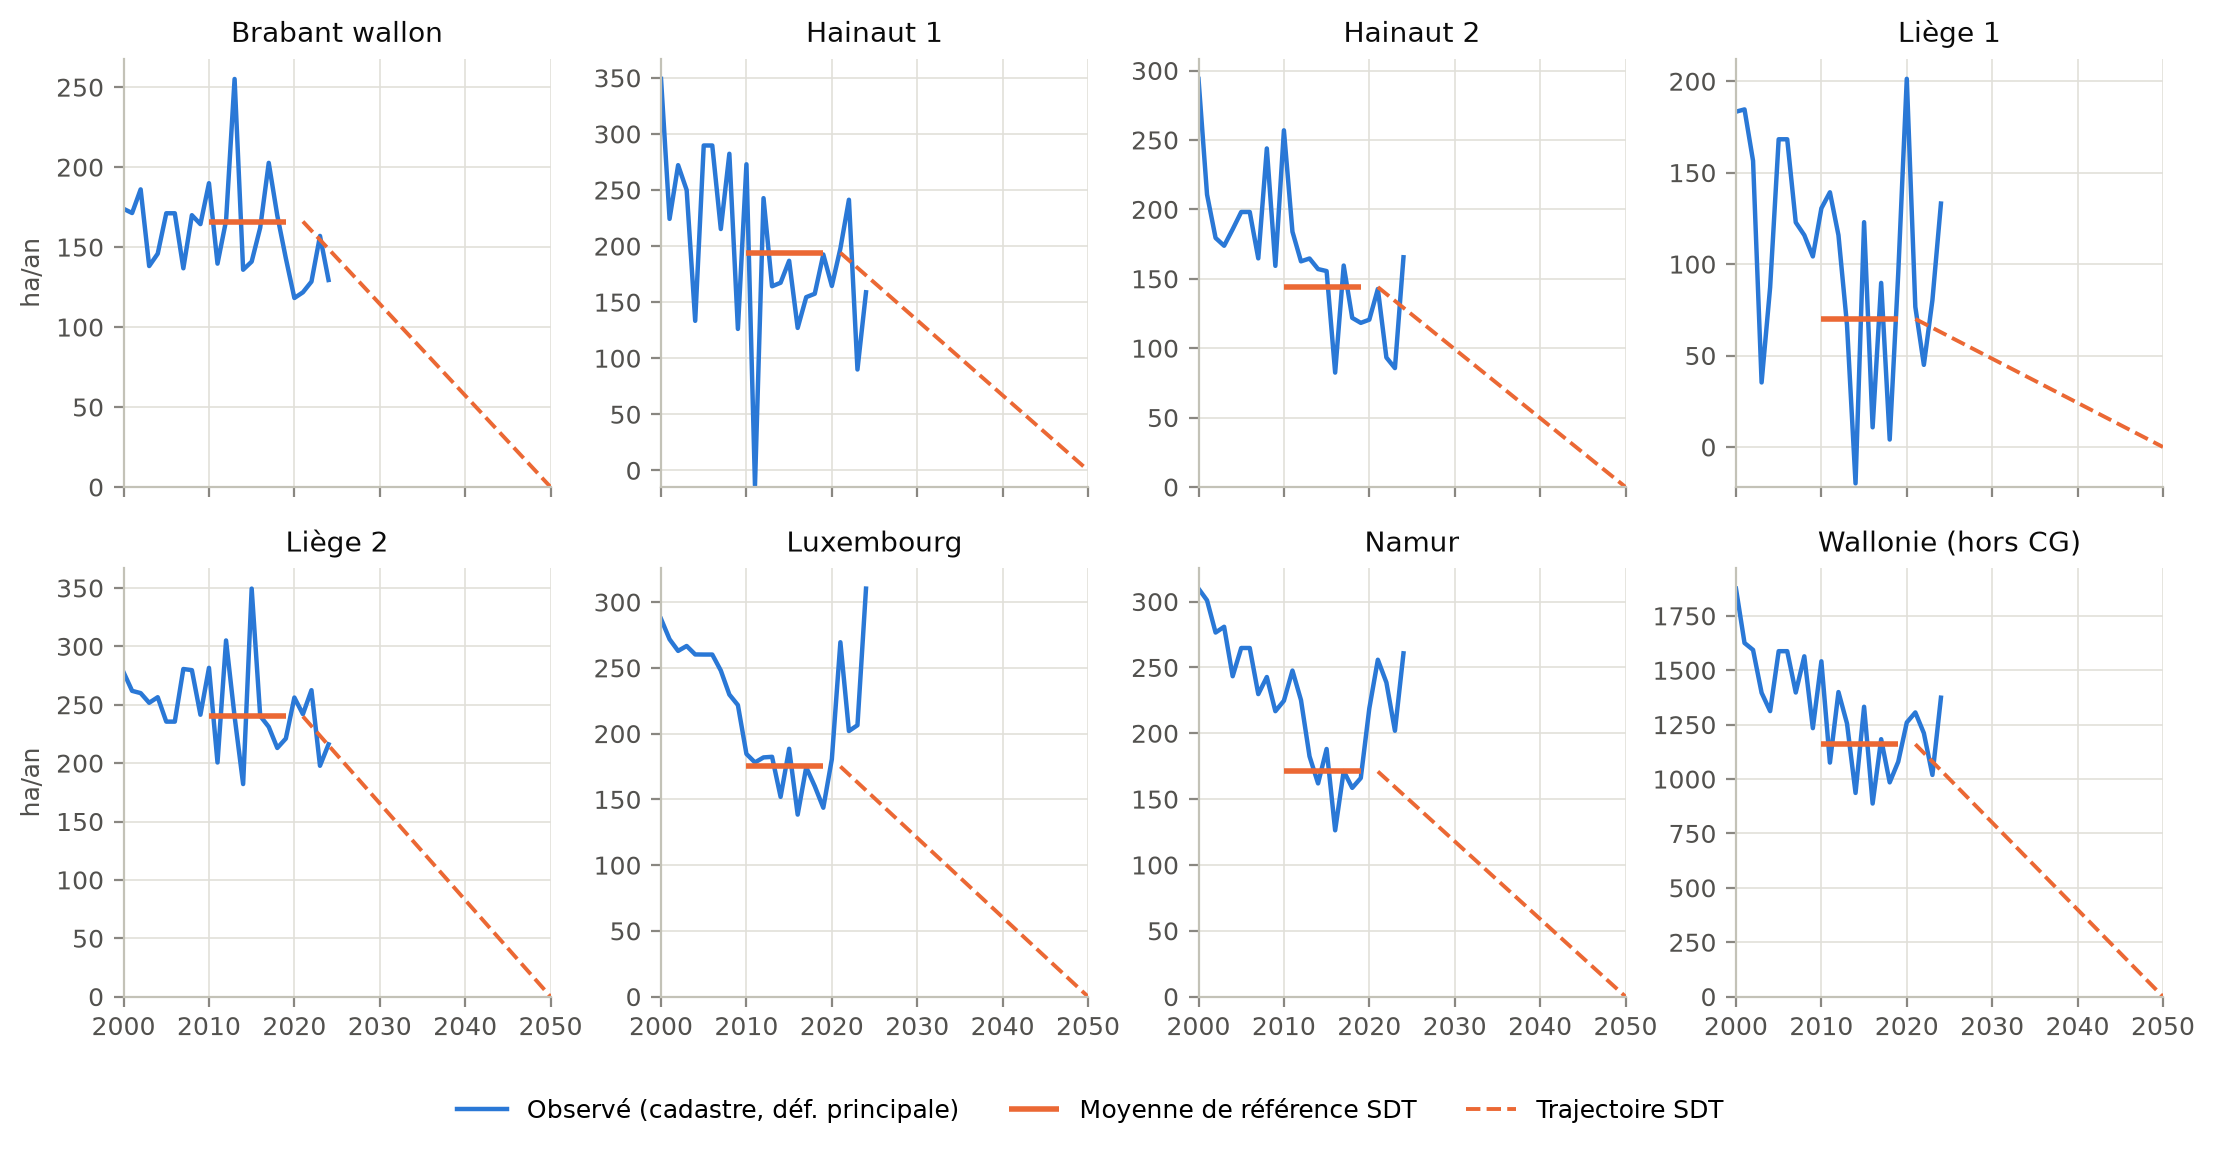
\includegraphics[width=\textwidth]{figures/bassins_series.png}
\caption{Consommation nette annuelle observée par bassin (2000-\AnneeFinObs), moyenne de référence et trajectoire du SDT. Les échelles verticales diffèrent d'un panneau à l'autre.}
\label{fig:bassins}
\end{figure}

\NbBassinsAuDessus{} bassins sur 7 sont au-dessus de leur trajectoire (tableau~\ref{tab:bassins}, figure~\ref{fig:bassins}). Trois profils se dégagent~:
\begin{itemize}
\item \textbf{Luxembourg et Namur}~: hausse franche de la consommation par rapport à la référence (\LuxObsMoy{} contre \LuxRef\haan{} et \NamObsMoy{} contre \NamRef\haan), au-delà de la variabilité passée ($z=\LuxZ$ et $\NamZ$, tableau~\ref{tab:variabilite}). Leurs dépassements cumulés représentent \LuxNamPartEcart\,\% du dépassement régional net, les marges des bassins sous la trajectoire compensant le reste. Une partie de la hausse luxembourgeoise tient à un saut à Arlon en \AnneeFinObs{} (section~\ref{sec:sauts})~; neutralisé, le ratio du Luxembourg reste de \LuxRatioNeutre.
\item \textbf{Liège~1 et Liège~2}~: Liège~1 est au-dessus de sa trajectoire (ratio \LUnRatio), mais ce ratio repose sur une référence faible (\LUnRef\haan, contre environ \LUnRefCpdt\haan{} dans la note de la CPDT) et une année \AnneeFinObs{} élevée~; avec la référence de la CPDT, il tombe à \LUnRatioRefCpdt{} (section~\ref{sec:cpdt})~; Liège~2 est à l'équilibre.
\item \textbf{Brabant wallon, Hainaut~1 et Hainaut~2}~: sous la trajectoire. Pour le Brabant wallon et le Hainaut~2, la baisse par rapport à la référence (\BWVarPct\,\% et \HDVarPct\,\%) est antérieure au SDT et proche du seuil de significativité.
\end{itemize}

\begin{table}[ht]
\centering\small
\caption{Variabilité interannuelle et changement de niveau de la consommation nette (ha/an). $z$~: écart des moyennes rapporté à son écart-type estimé (hypothèse H2).}
\label{tab:variabilite}
\begin{tabular}{lrrrrr}
\toprule
Bassin & \makecell{Moyenne\\2010-2019} & \makecell{Écart-type\\interannuel} & \makecell{Moyenne\\2021-2024} & Variation (\%) & $z$ \\
\midrule
Brabant wallon & 171 & 37 & 134 & \textminus{}21{,}3 & \textminus{}1{,}66 \\
Hainaut 1 & 165 & 76 & 172 & +4{,}1 & 0{,}15 \\
Hainaut 2 & 156 & 46 & 122 & \textminus{}22{,}1 & \textminus{}1{,}27 \\
Liège 1 & 75 & 58 & 84 & +10{,}9 & 0{,}24 \\
Liège 2 & 246 & 51 & 230 & \textminus{}6{,}8 & \textminus{}0{,}56 \\
Luxembourg & 168 & 18 & 247 & +46{,}7 & 7{,}25 \\
Namur & 185 & 37 & 239 & +29{,}2 & 2{,}47 \\
Wallonie (hors CG) & 1\,168 & 213 & 1\,227 & +5{,}1 & 0{,}47 \\
\bottomrule
\end{tabular}

\end{table}

\paragraph{Écart entre références} Le choix de la référence modifie la lecture du Hainaut~1 (\HUnRatio{} avec la référence du SDT, \HUnRatioRecalc{} avec la référence recalculée)~: le SDT retient pour ce bassin une moyenne plus élevée (\HUnRef{} contre \HUnRefRecalc\haan) que celle que donne le cadastre brut. L'écart provient vraisemblablement d'un traitement des natures cadastrales ou des reclassements différent du nôtre~; il ne peut être tranché sans la série officielle.

\section{Ce qui est artificialisé}
\begin{figure}[ht]
\centering
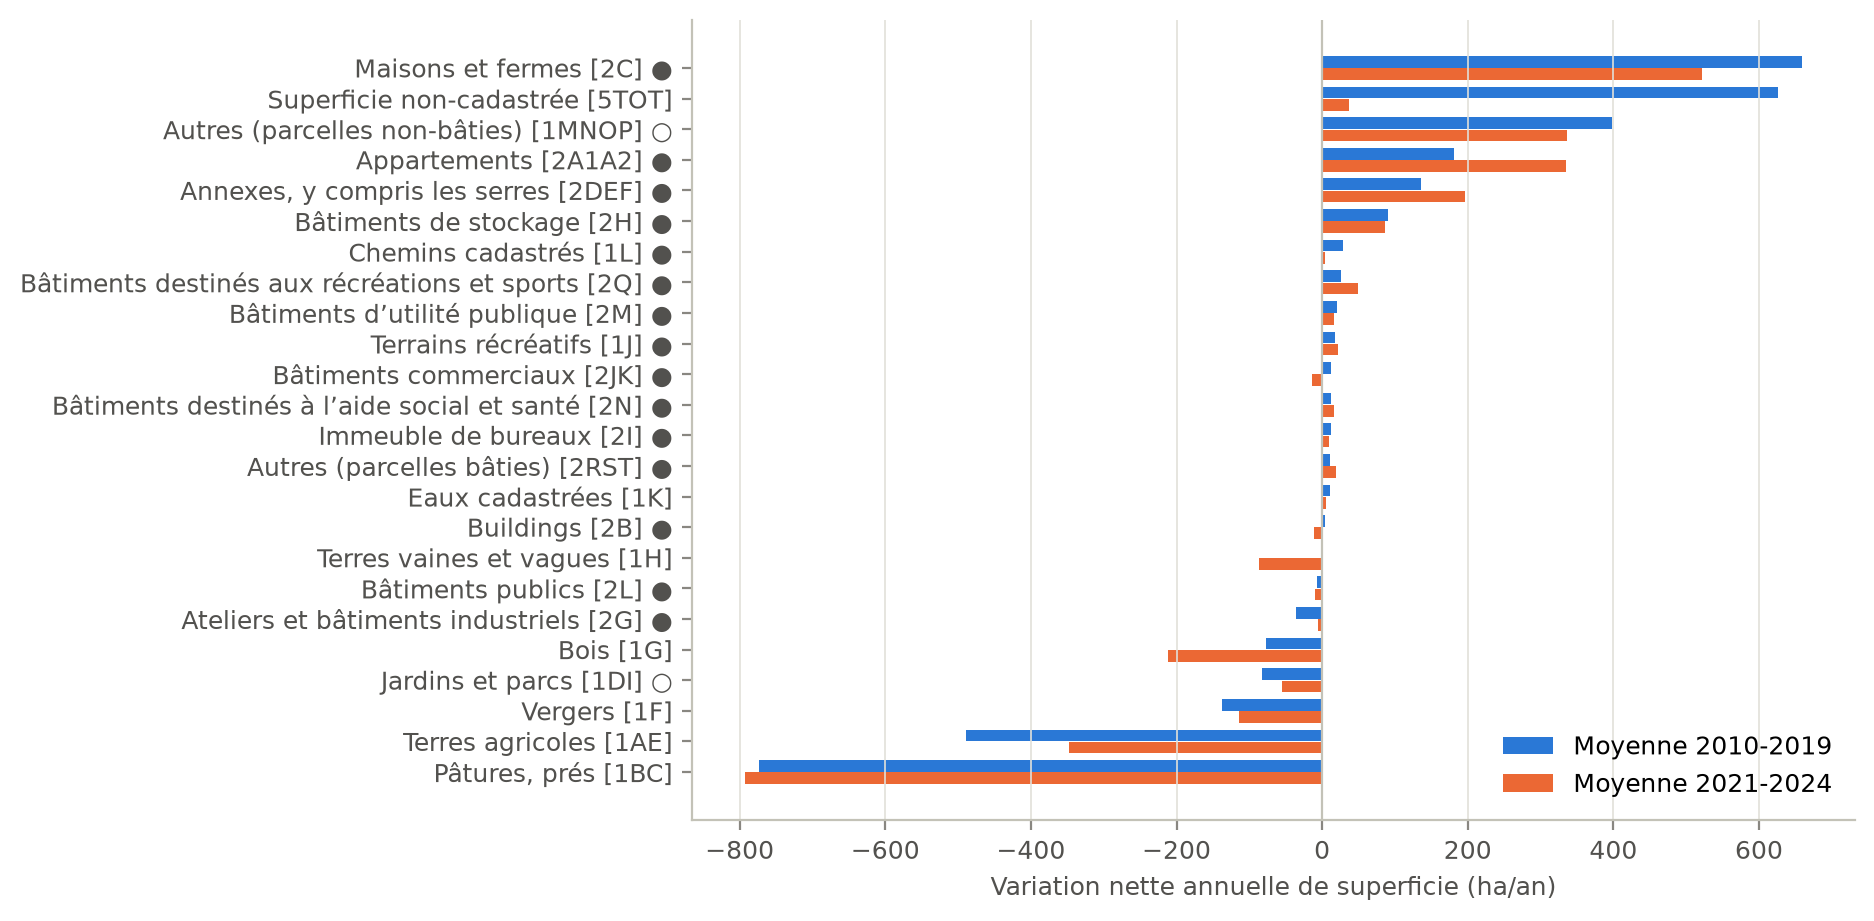
\includegraphics[width=0.92\textwidth]{figures/composition_rubriques.png}
\caption{Variation nette annuelle moyenne de superficie par rubrique cadastrale, Wallonie hors Communauté germanophone. $\bullet$~rubrique de la définition principale~; $\circ$~rubrique ajoutée dans la définition large. Rubriques dont la variation dépasse 8\haan{} sur l'une des périodes.}
\label{fig:composition}
\end{figure}

La décomposition par rubrique (figure~\ref{fig:composition}, annexe~\ref{ann:nomenclature}) montre trois évolutions~:
\begin{itemize}
\item \textbf{du pavillon vers l'appartement}~: les maisons et fermes reculent de \MaisonsRef{} à \MaisonsObs\haan, les appartements passent de \ApptRef{} à \ApptObs\haan, les annexes de \AnnexesRef{} à \AnnexesObs\haan~; la production de logements se densifie, sans réduire encore la surface totale~;
\item \textbf{l'intégration du non-cadastré s'est tarie}~: la superficie non cadastrée augmentait de \NonCadRef\haan{} en 2010-2019 (intégrations ponctuelles de domaine public au cadastre), contre \NonCadObs\haan{} depuis 2021. Hors définition, ce poste n'entre pas dans l'indicateur, mais il signale que la période de référence a connu des opérations administratives qui ont pu alimenter certaines rubriques bâties (cas de Blegny en 2020)~;
\item \textbf{des prélèvements plus forestiers}~: la diminution des bois s'accélère (\BoisRef{} $\rightarrow$ \BoisObs\haan), en partie par reclassements (Arlon).
\end{itemize}

\section{Communes}
\label{sec:communes}
\begin{figure}[p]
\centering
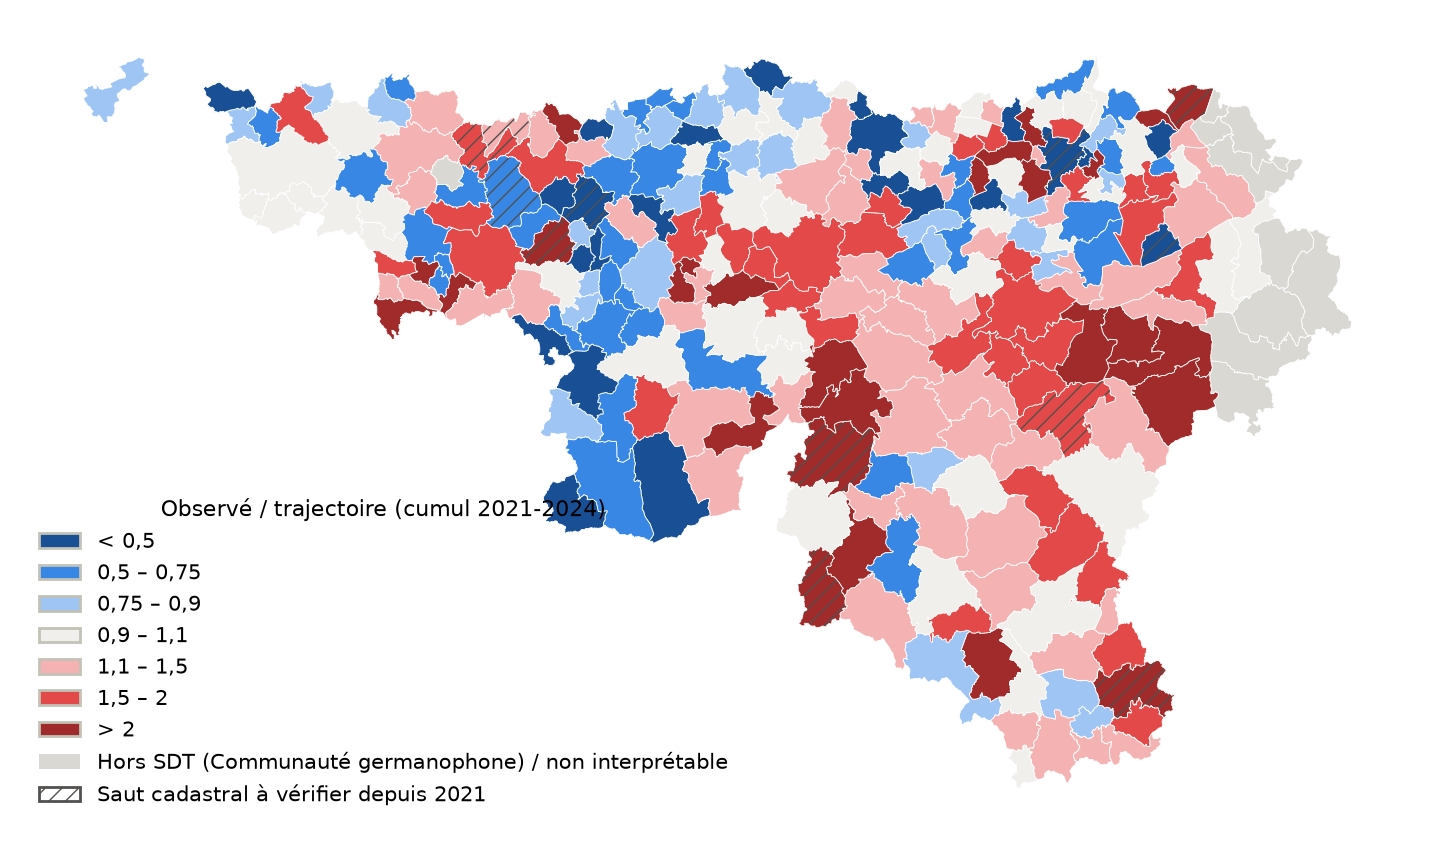
\includegraphics[width=\textwidth]{figures/carte_ratio_communes.png}
\caption{Ratio entre la consommation cumulée \AnneeDebutObs-\AnneeFinObs{} et le cumul autorisé par une trajectoire communale théorique (règle du SDT appliquée à la moyenne communale 2010-2019). Hachures~: commune présentant un saut cadastral à vérifier depuis 2021.}
\label{fig:carte_ratio}
\vspace{1em}
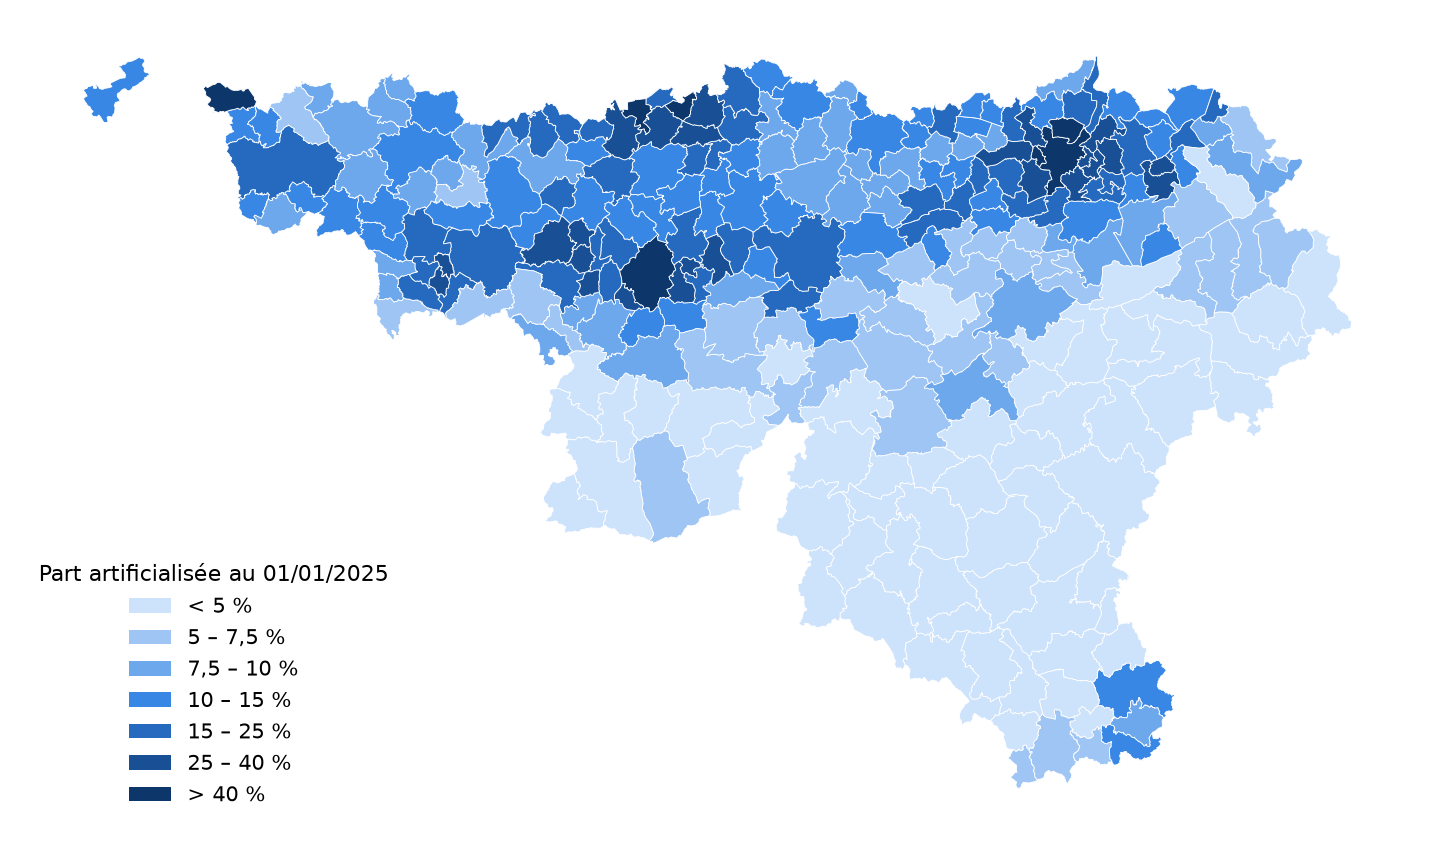
\includegraphics[width=0.86\textwidth]{figures/carte_part_artificialisee.png}
\caption{Part du territoire communal artificialisée (définition principale) au 01/01/\AnneeStock.}
\label{fig:carte_stock}
\end{figure}

Sur \NbCommunesSDT{} communes, \NbAuDessus{} sont au-dessus de leur trajectoire théorique, \NbDans{} dans la trajectoire et \NbNonInterp{} non interprétable (référence négative). La carte (figure~\ref{fig:carte_ratio}) reproduit le gradient des bassins~: dépassements fréquents dans le sud et l'est (Ardenne, Condroz, Famenne), marges dans le Brabant wallon et l'ouest du Hainaut. Elle ne recoupe pas la carte du niveau d'artificialisation (figure~\ref{fig:carte_stock})~: ce sont surtout des communes peu artificialisées qui dépassent leur trajectoire. Parmi le quart des communes les moins artificialisées, \PartAuDessusQuartBas\,\% sont au-dessus, contre \PartAuDessusQuartHaut\,\% dans le quart le plus artificialisé (corrélation de rang entre part artificialisée et ratio~: \CorrPartRatio).

\begin{figure}[ht]
\centering
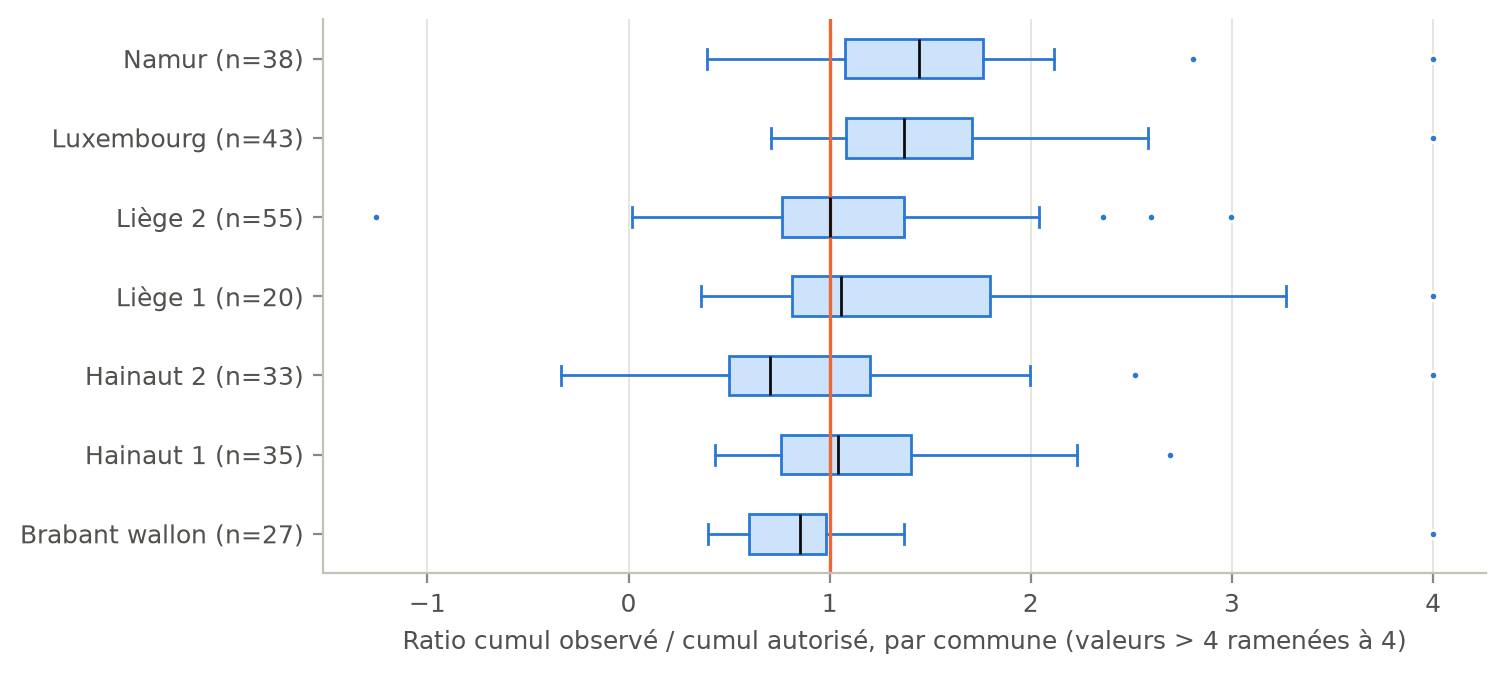
\includegraphics[width=0.9\textwidth]{figures/communes_ratios_boxplot.png}
\caption{Distribution des ratios communaux par bassin (boîte~: quartiles~; trait~: médiane).}
\label{fig:boxplot}
\end{figure}

\paragraph{Lire le ratio avec l'écart en hectares} Le ratio est instable lorsque la référence communale est faible~: \CommuneRatioMax{} affiche un ratio de \RatioMax{} pour une référence de \RefCommuneRatioMax\haan. Le tableau~\ref{tab:contributeurs} classe donc les communes par écart cumulé en hectares, qui mesure leur contribution réelle à l'écart régional.

\begin{table}[ht]
\centering\footnotesize
\caption{Communes contribuant le plus à l'écart, en hectares cumulés \AnneeDebutObs-\AnneeFinObs{} (trajectoire communale théorique). Ratio neutralisé~: après remplacement des années signalées par la médiane communale.}
\label{tab:contributeurs}
\begin{tabular}{llrrrrrl}
\toprule
Commune & Bassin & \makecell{Réf.\\(ha/an)} & \makecell{Obs.\\(ha/an)} & \makecell{Écart\\cumulé (ha)} & Ratio & \makecell{Ratio\\neutralisé} & \makecell{Saut(s)\\à vérifier} \\
\midrule
\multicolumn{8}{l}{\emph{Plus forts dépassements}} \\
\quad Arlon & Luxembourg & 8{,}2 & 38{,}1 & +121 & 4{,}91 & 1{,}34 & 2024 \\
\quad La Louvière & Hainaut 2 & 2{,}4 & 19{,}4 & +68 & 8{,}48 & 1{,}33 & 2024 \\
\quad Namur & Namur & 17{,}4 & 27{,}8 & +45 & 1{,}69 & 1{,}69 & -- \\
\quad Grâce-Hollogne & Liège 1 & 1{,}8 & 10{,}6 & +36 & 6{,}25 & 1{,}06 & -- \\
\quad Beauraing & Namur & 2{,}9 & 11{,}4 & +35 & 4{,}20 & 1{,}75 & 2021 \\
\quad Tubize & Brabant wallon & 1{,}0 & 8{,}6 & +31 & 9{,}27 & 2{,}19 & -- \\
\quad Plombières & Liège 2 & 5{,}9 & 13{,}2 & +30 & 2{,}36 & 1{,}44 & 2021 \\
\quad Dinant & Namur & 1{,}9 & 8{,}7 & +27 & 4{,}73 & 2{,}30 & -- \\
\quad Mons & Hainaut 1 & 8{,}6 & 14{,}5 & +25 & 1{,}78 & 0{,}72 & -- \\
\quad Vielsalm & Luxembourg & 3{,}9 & 9{,}5 & +23 & 2{,}58 & 2{,}58 & -- \\
\quad Vresse-sur-Semois & Namur & 1{,}2 & 6{,}5 & +21 & 5{,}63 & 1{,}31 & 2024 \\
\quad Theux & Liège 2 & 6{,}9 & 11{,}1 & +18 & 1{,}70 & 1{,}70 & -- \\
\multicolumn{8}{l}{\emph{Plus fortes marges}} \\
\quad Couvin & Namur & 21{,}7 & 8{,}0 & \textminus{}50 & 0{,}39 & 0{,}73 & -- \\
\quad Seneffe & Hainaut 2 & 7{,}2 & \textminus{}1{,}9 & \textminus{}35 & \textminus{}0{,}28 & 1{,}46 & 2023 \\
\quad Wanze & Liège 2 & 13{,}4 & 4{,}3 & \textminus{}33 & 0{,}34 & 0{,}79 & -- \\
\quad Les Bons Villers & Hainaut 2 & 8{,}7 & 0{,}5 & \textminus{}31 & 0{,}06 & 0{,}12 & -- \\
\quad Hannut & Liège 2 & 11{,}5 & 3{,}9 & \textminus{}28 & 0{,}36 & 0{,}53 & -- \\
\quad Liège & Liège 1 & 9{,}5 & 3{,}5 & \textminus{}22 & 0{,}39 & 1{,}37 & 2022 \\
\quad Saint-Ghislain & Hainaut 1 & 12{,}9 & 6{,}8 & \textminus{}22 & 0{,}56 & 0{,}85 & -- \\
\quad Sprimont & Liège 2 & 14{,}8 & 9{,}0 & \textminus{}20 & 0{,}64 & 0{,}64 & -- \\
\quad Thuin & Hainaut 2 & 10{,}5 & 5{,}0 & \textminus{}20 & 0{,}50 & 0{,}94 & -- \\
\quad Ecaussinnes & Hainaut 2 & 3{,}8 & \textminus{}1{,}2 & \textminus{}19 & \textminus{}0{,}34 & \textminus{}0{,}34 & -- \\
\quad Mouscron & Hainaut 1 & 8{,}3 & 3{,}4 & \textminus{}18 & 0{,}43 & 0{,}43 & -- \\
\quad Braine-le-Château & Brabant wallon & 8{,}9 & 4{,}0 & \textminus{}18 & 0{,}48 & 0{,}67 & -- \\
\bottomrule
\end{tabular}

\end{table}

\subsection{Sauts cadastraux à vérifier}
\label{sec:sauts}
\NbSautsSuivi{} communes présentent au moins une année signalée depuis 2021 (tableau~\ref{tab:sauts}), et \NbSautsRef{} au moins une durant la période de référence. Les cas examinés en détail confirment la nature administrative de plusieurs d'entre eux~: à Arlon, le saut de 2024 coïncide avec une hausse de \ArlonJ\ha{} des terrains récréatifs et une baisse de \ArlonG\ha{} des bois, soit un reclassement plutôt qu'un chantier~; à Enghien, une succession de reclassements entre pâtures et terres agricoles s'accompagne d'aller-retours dans les annexes bâties~; à Blegny, en 2020 (hors période de suivi), la superficie non cadastrée diminue de \BlegnyNC\ha{} tandis que les autres parcelles bâties augmentent de \BlegnyRST\ha. Neutraliser ces sauts fait basculer \NbBasculeHaut{} communes de \enquote{dans} à \enquote{au-dessus} et \NbBasculeBas{} en sens inverse~: le nombre de communes au-dessus de leur trajectoire est inchangé (\NbAuDessusNeutre), mais leur liste change.

\begin{table}[ht]
\centering\footnotesize
\caption{Communes présentant un saut cadastral à vérifier depuis 2021 (flux de l'année signalée et médiane communale, ha).}
\label{tab:sauts}
\begin{tabular}{llp{4.2cm}rll}
\toprule
Commune & Bassin & Année : flux (ha) & \makecell{Médiane\\2000-2024} & Statut & \makecell{Statut\\neutralisé} \\
\midrule
Enghien & Hainaut 1 & 2022 : +59, 2023 : \textminus{}31 & 6{,}3 & au-dessus & dans \\
Silly & Hainaut 1 & 2022 : +25 & 3{,}4 & au-dessus & au-dessus \\
La Louvière & Hainaut 2 & 2024 : +51 & 8{,}1 & au-dessus & au-dessus \\
Seneffe & Hainaut 2 & 2023 : \textminus{}28 & 5{,}1 & dans & au-dessus \\
Soignies & Hainaut 2 & 2022 : \textminus{}12 & 9{,}9 & dans & au-dessus \\
Liège & Liège 1 & 2022 : \textminus{}14 & 9{,}0 & dans & au-dessus \\
Plombières & Liège 2 & 2021 : +26 & 5{,}3 & au-dessus & au-dessus \\
Spa & Liège 2 & 2024 : \textminus{}14 & 1{,}7 & dans & dans \\
Arlon & Luxembourg & 2024 : +121 & 9{,}9 & au-dessus & au-dessus \\
La Roche-en-Ardenne & Luxembourg & 2021 : +20 & 4{,}3 & au-dessus & dans \\
Beauraing & Namur & 2021 : +22 & 5{,}8 & au-dessus & au-dessus \\
Vresse-sur-Semois & Namur & 2024 : +21 & 1{,}4 & au-dessus & au-dessus \\
\bottomrule
\end{tabular}

\end{table}

% ============================================================================
\chapter{Sensibilité aux choix de méthode}
\label{ch:sens}

Chaque choix des chapitres précédents a été remplacé par une alternative raisonnable, toutes choses égales par ailleurs (tableau~\ref{tab:sensibilite}, figure~\ref{fig:sensibilite}).

\begin{figure}[ht]
\centering
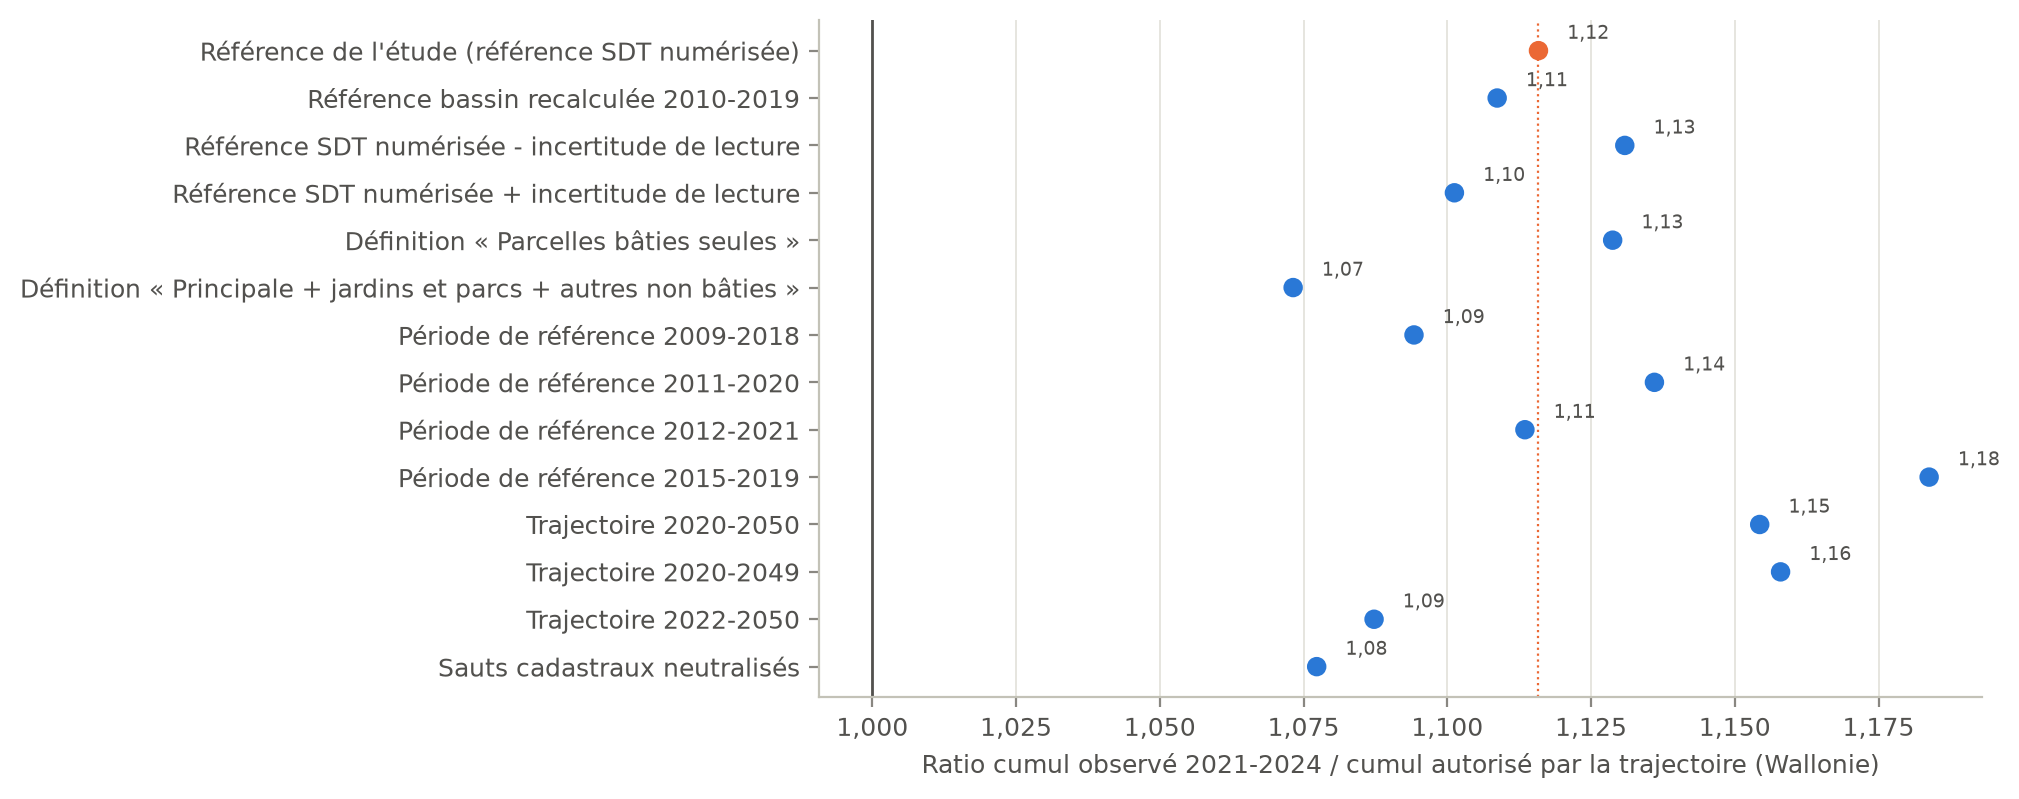
\includegraphics[width=0.95\textwidth]{figures/sensibilite_wallonie.png}
\caption{Ratio régional selon la variante de méthode. Point orange et ligne pointillée~: référence de l'étude~; ligne noire~: équilibre avec la trajectoire.}
\label{fig:sensibilite}
\end{figure}

\begin{table}[ht]
\centering\footnotesize
\caption{Ratio cumul observé / cumul autorisé selon les variantes de méthode, par bassin et pour la Wallonie, et nombre de communes au-dessus de leur trajectoire théorique.}
\label{tab:sensibilite}

\resizebox{\textwidth}{!}{\begin{tabular}{p{5.6cm}rrrrrrrrr}
\toprule
Variante & BW & H1 & H2 & L1 & L2 & Lux & Nam & Wal. & \makecell{Communes\\au-dessus} \\
\midrule
\multicolumn{10}{l}{\emph{Référence}} \\
\quad Référence de l'étude (référence SDT numérisée) & 0{,}85 & 0{,}93 & 0{,}89 & 1{,}26 & 1{,}01 & 1{,}49 & 1{,}48 & \textbf{1{,}12} & 144 \\
\multicolumn{10}{l}{\emph{Référence de bassin}} \\
\quad Référence bassin recalculée 2010-2019 & 0{,}83 & 1{,}10 & 0{,}82 & 1{,}17 & 0{,}98 & 1{,}55 & 1{,}36 & \textbf{1{,}11} & 144 \\
\multicolumn{10}{l}{\emph{Lecture des graphiques}} \\
\quad Référence SDT numérisée - incertitude de lecture & 0{,}86 & 0{,}95 & 0{,}91 & 1{,}30 & 1{,}02 & 1{,}51 & 1{,}49 & \textbf{1{,}13} & 144 \\
\quad Référence SDT numérisée + incertitude de lecture & 0{,}84 & 0{,}92 & 0{,}88 & 1{,}22 & 1{,}00 & 1{,}47 & 1{,}46 & \textbf{1{,}10} & 144 \\
\multicolumn{10}{l}{\emph{Définition}} \\
\quad Définition « Parcelles bâties seules » & 0{,}86 & 1{,}19 & 0{,}89 & 1{,}13 & 1{,}04 & 1{,}36 & 1{,}46 & \textbf{1{,}13} & 143 \\
\quad Définition « Principale + jardins et parcs + autres non bâties » & 0{,}74 & 1{,}17 & 0{,}90 & 0{,}63 & 0{,}83 & 1{,}44 & 1{,}72 & \textbf{1{,}07} & 120 \\
\multicolumn{10}{l}{\emph{Période de référence}} \\
\quad Période de référence 2009-2018 & 0{,}82 & 1{,}14 & 0{,}80 & 1{,}16 & 0{,}97 & 1{,}48 & 1{,}33 & \textbf{1{,}09} & 134 \\
\quad Période de référence 2011-2020 & 0{,}87 & 1{,}17 & 0{,}90 & 1{,}07 & 0{,}99 & 1{,}55 & 1{,}37 & \textbf{1{,}14} & 140 \\
\quad Période de référence 2012-2021 & 0{,}88 & 1{,}03 & 0{,}93 & 1{,}16 & 0{,}98 & 1{,}47 & 1{,}36 & \textbf{1{,}11} & 138 \\
\quad Période de référence 2015-2019 & 0{,}86 & 1{,}11 & 1{,}01 & 1{,}37 & 0{,}96 & 1{,}62 & 1{,}56 & \textbf{1{,}18} & 142 \\
\multicolumn{10}{l}{\emph{Calage de la trajectoire}} \\
\quad Trajectoire 2020-2050 & 0{,}88 & 0{,}97 & 0{,}92 & 1{,}30 & 1{,}04 & 1{,}54 & 1{,}53 & \textbf{1{,}15} & 150 \\
\quad Trajectoire 2020-2049 & 0{,}88 & 0{,}97 & 0{,}93 & 1{,}31 & 1{,}05 & 1{,}54 & 1{,}53 & \textbf{1{,}16} & 151 \\
\quad Trajectoire 2022-2050 & 0{,}83 & 0{,}91 & 0{,}87 & 1{,}23 & 0{,}98 & 1{,}45 & 1{,}44 & \textbf{1{,}09} & 135 \\
\multicolumn{10}{l}{\emph{Anomalies}} \\
\quad Sauts cadastraux neutralisés & 0{,}85 & 0{,}89 & 0{,}91 & 1{,}35 & 1{,}00 & 1{,}30 & 1{,}42 & \textbf{1{,}08} & 144 \\
\bottomrule
\end{tabular}
}
\end{table}

\paragraph{Ce qui est robuste} Le ratio régional reste supérieur à 1 dans toutes les variantes (\SensMin{} à \SensMax). Luxembourg et Namur sont au-dessus dans toutes les variantes, le Brabant wallon en dessous dans toutes, le Hainaut~2 en dessous dans \NbVarHDDessous{} variantes sur \SensNbVariantes{} et Liège~1 au-dessus dans \NbVarLUnDessus{} (avec la référence de la CPDT, son ratio n'est plus que de \LUnRatioRefCpdt, voir ci-dessous). Le nombre de communes au-dessus de leur trajectoire théorique varie entre \SensComMin{} et \SensComMax.

\paragraph{Ce qui est fragile} Le statut du Hainaut~1 et de Liège~2 dépend de la référence (SDT ou recalculée) et de la définition. L'amplitude du dépassement régional dépend surtout de la période de référence~: retenir 2015-2019, années de plus faible consommation, durcit la trajectoire (ratio \SensMax)~; la définition large, qui intègre des flux plus élevés en référence, l'adoucit (\SensMin).

\paragraph{Incertitudes externes} Les variantes ci-dessus ne modifient que les choix internes à l'étude. Trois variantes externes s'appuient sur la note préparatoire de la CPDT (section~\ref{sec:cpdt}).
\begin{itemize}
\item \emph{Étalonnage des données.} Retrancher de chaque année de suivi l'écart moyen 2021-2023 à la série CPDT/IWEPS (\CpdtEcartWal\haan) donne un ratio régional de \WalRatioCal.
\item \emph{Trajectoires de la CPDT.} Remplacer les références lues sur le SDT par celles qu'implique la note de la CPDT donne \WalRatioRefCpdt{} pour la Wallonie et \LUnRatioRefCpdt{} pour Liège~1.
\item \emph{Période.} Limiter le bilan à 2021-2023 donne \EtudeRatioTroisWal{} (étude) ou \CpdtRatioWal{} (CPDT).
\end{itemize}
Le constat qualitatif tient dans tous les cas~: la consommation ne décroît pas selon la pente de la trajectoire. Son \emph{ampleur} reste en revanche incertaine~: le dépassement va de \CpdtDepassPct{} à \WalDepassPct\,\% selon la période et la source.

% ============================================================================
\chapter{Discussion}
\label{ch:discussion}

\section{Que peut-on conclure~?}
\begin{enumerate}
\item \textbf{Les quatre premières années ne suivent pas la pente de la trajectoire.} L'écart est modéré (\WalDepassPct\,\% sur 2021-\AnneeFinObs, \CpdtDepassPct{} à \EtudeDepassTroisPct\,\% sur 2021-2023 selon la source), mais il s'accumule~: si la consommation restait au niveau moyen observé (\WalObsMoy\haan), l'écart cumulé atteindrait environ \WalEcartProj\ha{} en 2030.
\item \textbf{Ce n'est pas un échec du SDT}, entré en vigueur en août 2024~: les flux cadastraux 2021-2024 traduisent pour l'essentiel des projets autorisés avant lui, dans un contexte de rattrapage post-COVID. Le bilan est une mesure du point de départ.
\item \textbf{La géographie de l'écart est nette}~: elle désigne les bassins Luxembourg et Namur comme prioritaires pour l'analyse des causes (pression résidentielle liée au Grand-Duché de Luxembourg, zones d'activité, tourisme et résidences secondaires~?), hypothèses que les données mobilisées ici ne permettent pas de départager.
\end{enumerate}

\section{Registre des choix et hypothèses}
\begin{table}[ht]
\centering\small
\caption{Registre des choix (C) et hypothèses (H), avec leur effet mesuré ou attendu.}
\label{tab:registre}
\begin{tabular}{p{0.6cm}p{5.0cm}p{4.3cm}p{4.6cm}}
\toprule
& Énoncé & Effet sur les conclusions & Pour le lever \\
\midrule
C1 & Cadastre Statbel comme source & Usage déclaré, décalage temporel & Croisement WalOUS, permis \\
C2 & Trajectoire linéaire 2021-2050 & Ratio régional \SensCalageMin{} à \SensCalageMax{} selon calage & Valeurs officielles du SDT \\
C3 & Définition principale & Ratio \SensDefLarge{} (large) à \SensDefBati{} (bâti)~; \WalRatioCal{} si étalonné sur la CPDT/IWEPS & Natures cadastrales détaillées (IWEPS) \\
C4 & Année $N$ = stock $N+1$ $-$ stock $N$ & Validé ($r$ \ValPrincCorr{} contre \ValPrincCorrLag) & -- \\
C5 & Référence de bassin lue sur le SDT & Hainaut~1~: \HUnRatio{} ou \HUnRatioRecalc~; Liège~1~: \LUnRatio{} ou \LUnRatioRefCpdt{} (réf. CPDT) & Série officielle SA1.M1 \\
C6 & Trajectoire communale théorique & Statut communal descriptif & Trajectoires des SDC \\
C7 & Sauts signalés, non corrigés & \NbStatutsModifies{} statuts communaux modifiés & Vérification parcellaire AGDP \\
H1 & Réduction uniforme entre communes & Non mesurable ici & Politique de centralités \\
H2 & Années indépendantes (test $z$) & Significativité surestimée & Modèle de séries temporelles \\
H3 & Lecture des graphiques fidèle & $\pm$\IncertLecture\haan{}, ratio $\pm$\SensLectureDelta & Publication des valeurs \\
H4 & Domaine non cadastré stable & Voiries nouvelles ignorées & Données PICC / voiries \\
H5 & Décalage cadastral constant & Flux 2021-24 = projets antérieurs & Permis géolocalisés \\
\bottomrule
\end{tabular}
\end{table}

\section{Limites}
\label{sec:limites}
\paragraph{Artificialisation n'est pas imperméabilisation} L'indicateur cadastral compte une parcelle bâtie entière~; une maison sur un terrain de 10 ares artificialise 10 ares, dont une faible part est imperméable. La directive européenne vise davantage l'imperméabilisation et l'enlèvement de sol~; son suivi requerra une source d'observation de la Terre.
\paragraph{Artificialisation nette, pas brute} Le cadastre fournit des soldes par rubrique~: une désartificialisation (démolition et retour en prairie) et une artificialisation dans la même commune s'annulent. La compensation prévue par SA1.P9 ne peut donc pas être suivie séparément.
\paragraph{Économique sous-représenté} Les terrains industriels non bâtis, parkings et chantiers relèvent de la rubrique 1MNOP, exclue de la définition principale. L'annexe CPDT recense pourtant 2\,445\ha{} de foncier économique artificialisés entre 2012 et 2024 (environ 200\haan)~\citep{cpdt2025}. La variante \enquote{large} ne modifie pas le diagnostic régional, mais une analyse spécifique de ce segment nécessiterait les natures détaillées.
\paragraph{Courte période} Quatre années ne permettent pas d'estimer une tendance~; le diagnostic est un écart de niveau.
\paragraph{Communauté germanophone} Ses neuf communes sont hors champ du SDT~; elles figurent dans les fichiers produits mais pas dans les résultats.

\section{Autres approches possibles}
\begin{itemize}
\item \textbf{Indicateur IWEPS exact} -- reclasser les 216 natures cadastrales (données AGDP non ouvertes) pour reproduire la définition officielle.
\item \textbf{Observation de la Terre} -- WalOUS (2018 et suivants) ou Copernicus pour mesurer la couverture physique et l'imperméabilisation, au prix d'une série plus courte et d'une autre définition.
\item \textbf{Permis} -- mesurer l'artificialisation \emph{autorisée}, sans décalage, une fois les permis dématérialisés et géolocalisés.
\item \textbf{Normalisation} -- rapporter la consommation aux ménages ou aux emplois supplémentaires pour distinguer efficacité foncière et dynamisme démographique.
\item \textbf{Trajectoire non linéaire} -- le SDT n'impose pas la forme de la décroissance~; une trajectoire exponentielle ou par paliers donnerait d'autres plafonds intermédiaires pour le même objectif 2050.
\end{itemize}

% ============================================================================
\chapter{Recommandations et pistes}
\label{ch:reco}

\section{Pour les producteurs de données et le suivi régional}
\begin{enumerate}[label=\textbf{R\arabic*}]
\item \textbf{Publier les trajectoires en valeurs.} Un tableau des moyennes de référence et des plafonds annuels par bassin éviterait toute reconstitution et fixerait la convention de calage (départ 2020 ou 2021, zéro en 2049 ou 2050). Il est d'autant plus nécessaire que le graphique du SDT et la note de la CPDT ne partent pas de la même valeur pour Liège~1 (\LUnRef{} contre environ \LUnRefCpdt\haan).
\item \textbf{Publier le monitoring SA1.M1 en données ouvertes}, sous forme de série annuelle par bassin et par commune, avec la méthode.
\item \textbf{Actualiser la série communale ouverte de l'IWEPS} (arrêtée au 01/01/2023 sur l'API, alors que la fiche régionale va jusqu'au 01/01/2026), la publier en hectares et rétablir le téléchargement Walstat (lien rompu lors des consultations des 27/10 et 06/11/2026).
\item \textbf{Documenter les reclassements cadastraux} (registre des opérations de mise à jour de masse de l'AGDP), pour séparer artificialisation réelle et artefacts.
\item \textbf{Développer l'indicateur fondé sur les permis}, comme le recommande la CPDT, pour mesurer l'effet du SDT sans attendre l'enregistrement cadastral.
\item \textbf{Publier les données du rapport triennal.} Diffuser, avec le premier rapport triennal, les séries annuelles par bassin et par commune qui le fondent, en tableaux et non seulement en graphiques. Des travaux indépendants comme celui-ci pourraient alors être réconciliés directement avec la référence officielle.
\item \textbf{Ouvrir l'accès aux données des indicateurs.} Plusieurs indicateurs proposés par la CPDT reposent sur des données à accès restreint (matrice cadastrale parcellaire, registre national géolocalisé, transactions) ou non structurées (permis). L'annexe~\ref{ann:indicateurs} détaille, indicateur par indicateur, les données nécessaires et les moyens de les rendre disponibles.
\end{enumerate}

\section{Pour les communes}
\begin{enumerate}[label=\textbf{R\arabic*},resume]
\item \textbf{Utiliser la trajectoire théorique comme point de départ} de la trajectoire du schéma de développement communal, en justifiant les écarts par la politique de centralités.
\item \textbf{Vérifier les années signalées} (tableau~\ref{tab:sauts} et annexe~\ref{ann:communes}) avec les services du cadastre avant toute communication.
\end{enumerate}

\section{Pistes de prolongement de l'étude}
\begin{itemize}
\item mise à jour automatique à chaque publication Statbel (relancer \fichier{run\_all.py --refresh})~;
\item suivi de la part de logements neufs en centralité (SA2.P2), dont les valeurs 2010-2020 par bassin ont déjà été numérisées (tableau~\ref{tab:sdt})~;
\item croisement avec WalOUS pour les communes en dépassement~;
\item extension à la Flandre (\emph{ruimtebeslag}) et à Bruxelles avec le même cadre de transparence~;
\item analyse explicative des dépassements luxembourgeois et namurois (démographie, zones d'activité, résidences secondaires).
\end{itemize}

% ============================================================================
\appendix

\chapter{Nomenclature cadastrale et composition}
\label{ann:nomenclature}
\begin{table}[ht]
\centering\small
\caption{Rubriques du registre cadastral (Statbel), inclusion dans les définitions et variation nette moyenne (Wallonie hors Communauté germanophone).}
\label{tab:composition}
\begin{tabular}{llcrr}
\toprule
Code & Rubrique cadastrale (Statbel) & \makecell{Incluse dans\\la définition} & \makecell{2010-2019\\(ha/an)} & \makecell{2021-2024\\(ha/an)} \\
\midrule
1AE & Terres agricoles & -- & \textminus{}489{,}4 & \textminus{}348{,}3 \\
1BC & Pâtures, prés & -- & \textminus{}773{,}2 & \textminus{}792{,}4 \\
1DI & Jardins et parcs & large & \textminus{}82{,}5 & \textminus{}54{,}7 \\
1F & Vergers & -- & \textminus{}138{,}0 & \textminus{}113{,}7 \\
1G & Bois & -- & \textminus{}76{,}7 & \textminus{}211{,}9 \\
1H & Terres vaines et vagues & -- & 0{,}2 & \textminus{}86{,}0 \\
1J & Terrains récréatifs & principale & 17{,}2 & 22{,}1 \\
1K & Eaux cadastrées & -- & 11{,}3 & 5{,}6 \\
1L & Chemins cadastrés & principale & 28{,}5 & 4{,}6 \\
1MNOP & Autres (parcelles non-bâties) & large & 398{,}1 & 336{,}5 \\
2A1A2 & Appartements & principale & 181{,}0 & 334{,}8 \\
2B & Buildings & principale & 3{,}7 & \textminus{}11{,}5 \\
2C & Maisons et fermes & principale & 659{,}1 & 521{,}9 \\
2DEF & Annexes, y compris les serres & principale & 135{,}2 & 195{,}9 \\
2G & Ateliers et bâtiments industriels & principale & \textminus{}35{,}3 & \textminus{}5{,}4 \\
2H & Bâtiments de stockage & principale & 90{,}5 & 85{,}7 \\
2I & Immeuble de bureaux & principale & 11{,}9 & 9{,}0 \\
2JK & Bâtiments commerciaux & principale & 12{,}6 & \textminus{}14{,}6 \\
2L & Bâtiments publics & principale & \textminus{}6{,}7 & \textminus{}10{,}1 \\
2M & Bâtiments d’utilité publique & principale & 20{,}1 & 15{,}9 \\
2N & Bâtiments destinés à l’aide social et santé & principale & 12{,}2 & 16{,}8 \\
2O & Bâtiments destinés à l’enseignement, recherche et culture & principale & 2{,}5 & \textminus{}2{,}7 \\
2P & Bâtiments destinés aux cultes & principale & \textminus{}2{,}7 & \textminus{}3{,}1 \\
2Q & Bâtiments destinés aux récréations et sports & principale & 26{,}3 & 49{,}8 \\
2RST & Autres (parcelles bâties) & principale & 11{,}4 & 18{,}5 \\
3TOT & Parcelles non-normalisées & -- & 0{,}0 & 0{,}0 \\
5TOT & Superficie non-cadastrée & -- & 626{,}6 & 37{,}3 \\
\bottomrule
\end{tabular}

\end{table}

\chapter{Trajectoires numérisées du SDT}
\label{ann:sdt}
\begin{figure}[ht]
\centering
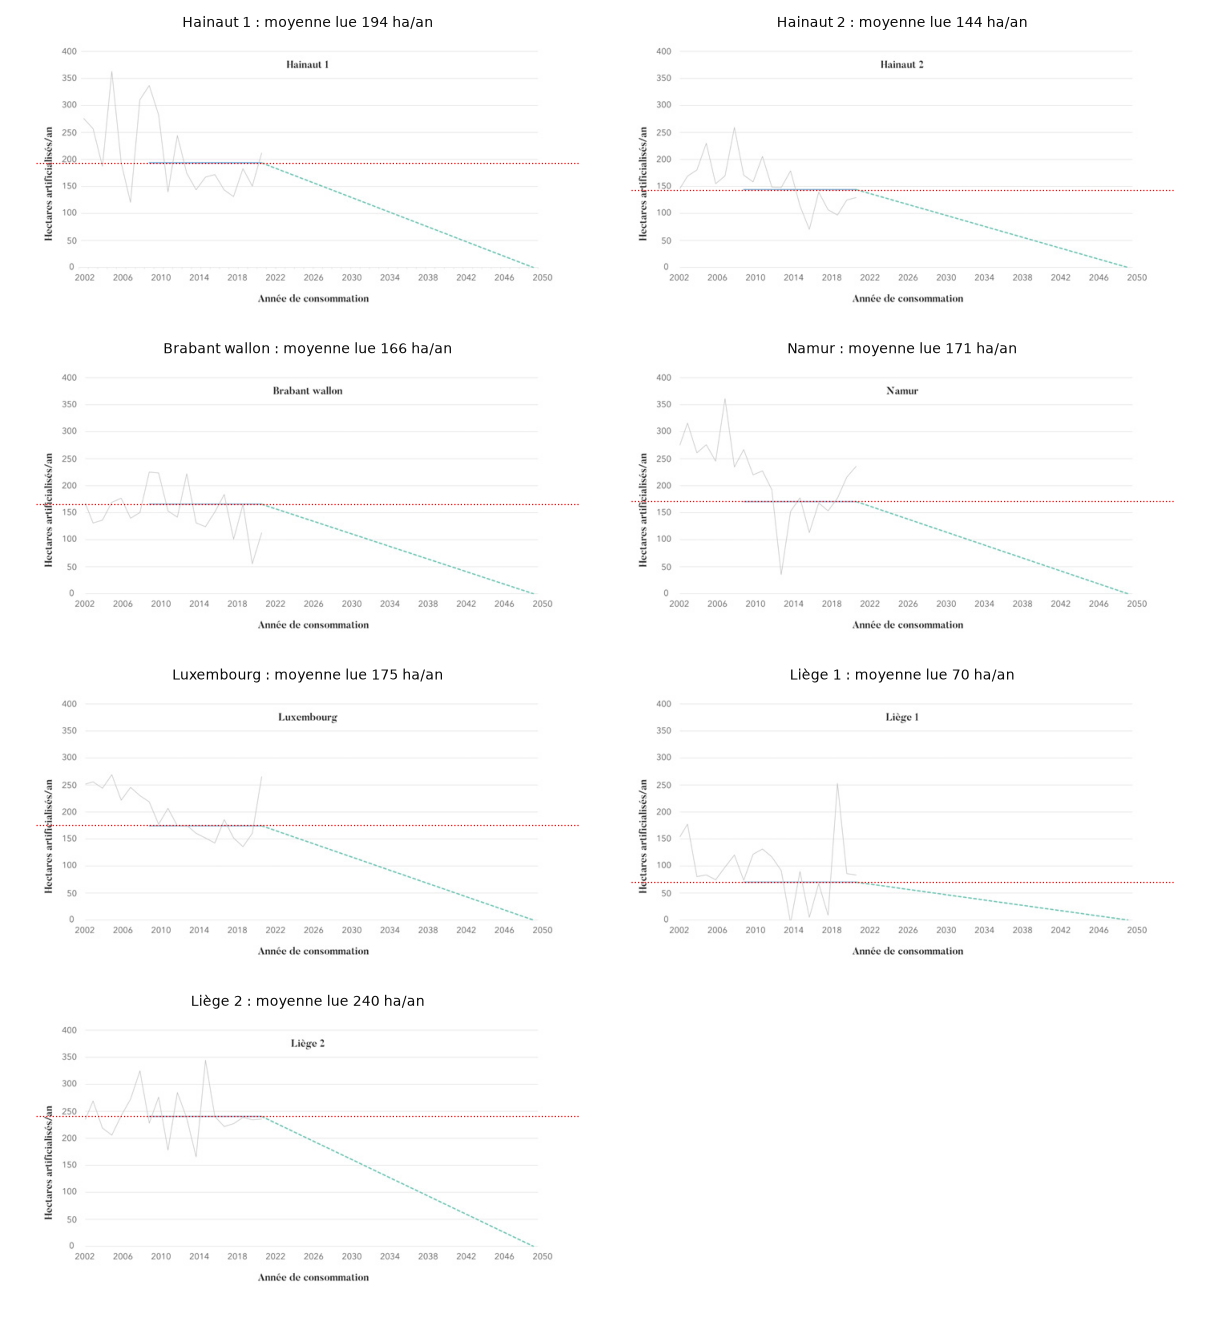
\includegraphics[width=\textwidth]{figures/sdt_numerisation.png}
\caption{Planche de contrôle de la numérisation~: graphiques originaux du SDT (p.~40-42) et moyenne lue (pointillé rouge).}
\label{fig:qa}
\end{figure}
Les valeurs numérisées sont versionnées dans \fichier{references/trajectoires\_sdt\_2024\_bassins.csv}, et les séries historiques lues dans \fichier{data/processed/sdt\_series\_historiques\_numerisees.csv}.

\chapter[Indicateurs du rapport triennal]{Indicateurs du rapport triennal~: données nécessaires et faisabilité}
\label{ann:indicateurs}
Cette annexe reprend les indicateurs proposés par la CPDT pour le rapport triennal~\citep{cpdt_monitoring2025}. Pour chacun, elle indique les données nécessaires, leur accessibilité et la difficulté de le produire. Les appréciations de difficulté sont celles de l'auteur~; l'accessibilité est décrite d'après les documents publics consultés en novembre 2026 et devra être confirmée auprès des détenteurs. Le SPF Finances publie d'autres jeux ouverts (transactions, baux, droits des personnes morales) que nous n'avons pas examinés~: les indicateurs de prix et de propriété publique classés ci-dessous sous convention pourraient être plus accessibles qu'indiqué. Trois niveaux d'accès sont distingués~: \textbf{ouvert} (téléchargeable librement)~; \textbf{convention} (données existantes, accessibles à des institutions sous protocole, par exemple l'IWEPS pour la matrice cadastrale)~; \textbf{à créer} (données qui n'existent pas sous forme exploitable).

{\scriptsize
\setlength{\tabcolsep}{3pt}
\begin{longtable}{>{\raggedright\arraybackslash}p{0.5cm}>{\raggedright\arraybackslash}p{3.3cm}>{\raggedright\arraybackslash}p{5.3cm}>{\raggedright\arraybackslash}p{1.5cm}>{\raggedright\arraybackslash}p{4.6cm}}
\caption{Indicateurs proposés par la CPDT, données nécessaires et faisabilité.}\label{tab:indicateurs}\\
\toprule
& Indicateur & Données nécessaires (détenteur~; accès) & Difficulté & Obstacle principal et piste \\
\midrule
\endfirsthead
\toprule
& Indicateur & Données nécessaires (détenteur~; accès) & Difficulté & Obstacle principal et piste \\
\midrule
\endhead
\bottomrule
\endfoot
\multicolumn{5}{l}{\textbf{A. Suivi de l'action publique} (non calculés dans la note préparatoire)}\\
A1 & Communes couvertes par un SDC ou un SDP, dont \enquote{optimisation spatiale} & Registre des schémas communaux adoptés et en cours (SPW TLPE~; périmètres ouverts, état d'avancement interne) & Faible & Publier annuellement le registre, avec la date d'adoption et le volet \enquote{optimisation spatiale} \\
A2 & Superficie par affectation au plan de secteur & Plan de secteur vectoriel (SPW~; ouvert) à dates successives, registre des révisions & Faible & Mesurer une évolution exige des versions datées~: archiver un millésime par an \\
A3 & Permis octroyés chaque année & Statistiques des permis de bâtir par commune (Statbel~; ouvert)~; permis d'urbanisme individuels (communes, fonctionnaires délégués~; non centralisés) & Faible (commune), élevée (centralités) & Pas de base régionale géolocalisée des permis~: elle viendra de la dématérialisation \\
A4 & Permis pour logements neufs et rénovation, par type & Statbel distingue construction neuve et rénovation, nombre de logements, appartements (ouvert, par commune) & Faible (commune), élevée (centralités) & Idem A3~; l'échelle communale est disponible dès aujourd'hui \\
A5 & Permis pour nouveaux commerces, par type & Permis d'implantation commerciale, surfaces de vente et type (SPW EER~; non obtenus par la CPDT~; la base LOGIC ne contient ni surface ni type) & Élevée & Convention avec la Direction des implantations commerciales ou ajout des champs dans LOGIC \\
A6 & Part de pleine terre dans les permis résidentiels & Surfaces de pleine terre et imperméabilisées des projets (dossiers de permis~; à créer) & Élevée & Information non structurée~: champ obligatoire dans les formulaires de demande dématérialisés \\
A7 & Projets de conversion de sites à réaménager (SAR) & Inventaire des SAR et arrêtés (SPW TLPE~; ouvert pour l'inventaire), financements & Faible à moyenne & Statut d'avancement des projets à documenter~; la CPDT travaille à qualifier l'inventaire \\
A8 & Opérations de développement urbain & Liste et périmètres des opérations (SPW~; administratif) & Faible & Peu d'opérations~: simple tableau administratif \\
\addlinespace
\multicolumn{5}{l}{\textbf{B. Suivi de l'impact territorial} (calculés par la CPDT avec les données de l'IWEPS)}\\
B1 & Superficie artificialisée, non artificialisée et de nature inconnue & Catégories d'utilisation du sol par commune (IWEPS~; API ouverte, jusqu'au 01/01/2023)~; natures cadastrales par commune et par secteur statistique (SPF Finances~; ouvert)~; approximation par les rubriques Statbel (ouvert, présente étude)~; centralités~: nature cadastrale par parcelle (matrice AGDP~; convention) et plan parcellaire (ouvert) & Faible (commune), élevée (centralités) & Actualiser la série communale de l'IWEPS et diffuser celle par centralité \\
B2 & Superficie artificialisée par catégorie d'utilisation & Natures cadastrales par commune (SPF Finances~; ouvert) et table de passage vers les 16 catégories~; parts par catégorie (IWEPS~; API ouverte, jusqu'au 01/01/2023) & Faible à moyenne & Publier la table de passage nature par nature, que nous n'avons pas trouvée \\
B3 & Évolution annuelle nette, comparée aux trajectoires & Données de B1 et trajectoires chiffrées par bassin & Faible & Réalisé dans cette étude avec Statbel~; publier les trajectoires en tableau (R1) \\
B4 & Superficie imperméabilisée par catégorie & WalOUS 2020 et 2023 (ouvert), PICC (ouvert, mis à jour en continu), catégories parcellaires (convention) & Moyenne (bassins), élevée (catégories) & Saison des prises de vue, couvert arboré, voiries hors cadastre~: acquisitions à saison fixe et archivage daté du PICC \\
B5 & Nombre et type de logements & Statistique cadastrale du parc de bâtiments (Statbel~; ouvert, par commune) & Faible & -- \\
B6 & Évolution annuelle nette des logements par type & Idem B5, millésimes successifs & Faible & Production nette et non par année de construction, comme le recommande la CPDT \\
B7 & Population et superficie résidentielle comparées & Population et ménages (Statbel~; ouvert), superficie résidentielle (B2) & Faible & -- \\
B8 & Habitants en centralités et hors centralités & Registre national géolocalisé (convention, IWEPS)~; approximation par secteur statistique ou grille de 1\,km (Statbel~; ouvert) & Moyenne (approx.), élevée (exact) & Les secteurs ne suivent pas les limites des centralités~: diffuser l'agrégat par centralité \\
B9 & Ménages en centralités et hors centralités & Idem B8 & Moyenne à élevée & Idem B8 \\
B10 & Logements en centralités et hors centralités & Nombre de logements par parcelle (matrice AGDP~; convention) & Élevée & Diffuser l'agrégat calculé par l'IWEPS \\
B11 & Évolution nette de la part de logements en centralité, comparée à la trajectoire SA2.P2 & Deux millésimes de la matrice parcellaire (convention), centralités versionnées & Élevée & Indicateur central du second objectif du SDT (75\,\%)~; dépend aussi de la révision des centralités par les SDC \\
B12 & Terres non artificialisées en zones urbanisables, par affectation & Plan de secteur (ouvert) et couche \enquote{terrains non urbanisés} de l'IWEPS (dérivée de la matrice~; diffusion à vérifier) & Moyenne & Diffuser la couche ou ses agrégats par commune et par centralité \\
B13 & Aptitude à la construction des terrains destinés à l'habitat & B12, contraintes (aléa d'inondation, karst, éboulements, Natura 2000, réserves naturelles~; ouvert), voiries du PICC (ouvert) & Moyenne & Données ouvertes, mais traitement SIG lourd (méthode de la DAL) \\
B14 & \emph{(optionnel)} Terrains destinés à l'habitat appartenant au secteur public & Propriétaires des parcelles (matrice~; convention), base CPDT des propriétés publiques & Élevée & Données de propriété protégées~; agrégats publiables \\
B15 & Prix moyens des terrains destinés à l'habitat & Transactions (SPF Finances~; convention)~; prix moyens des terrains à bâtir par commune (Statbel, disponibilité récente à vérifier) & Moyenne (commune), élevée (centralités) & Accès aux transactions individuelles \\
B16 & Aptitude à la construction des terrains destinés à l'activité économique & Idem B13 & Moyenne & Idem B13 \\
B17 & \emph{(optionnel)} Terrains destinés à l'activité économique appartenant au secteur public & Idem B14 & Élevée & Idem B14 \\
B18 & Prix moyens des terrains destinés à l'activité économique & Transactions (convention)~; peu de ventes par bassin & Élevée & Faible nombre d'observations~: intervalles de confiance larges \\
\addlinespace
-- & \emph{(abandonné)} Localisation des commerces par rapport aux centralités & Surface de vente et type de commerce (SPW EER~; non disponibles) & -- & Abandonné par la CPDT faute de données \\
\end{longtable}
}

\section{Ce que cela implique}
Les indicateurs se répartissent en trois groupes.
\begin{enumerate}
\item \textbf{Calculables dès aujourd'hui avec des données ouvertes}, au moins à l'échelle communale~: A1, A2, A3 et A4 (par commune), A7, A8, B3, B5 à B7, B1 et B2 grâce aux natures cadastrales du SPF Finances, ainsi que B12, B13 et B16 en approximation. Un monitoring communal \enquote{léger}, reproductible et public, est donc possible sans nouvelle donnée~; la présente étude en couvre l'indicateur B3.
\item \textbf{Calculables sous convention}~: B1 et B2 par centralité, B4 par catégorie, B8 à B11, B14, B15, B17 et B18. Les données existent et l'IWEPS y a déjà accès. L'enjeu n'est pas de les produire, mais d'en diffuser les agrégats (par commune, par bassin, par centralité), qui ne posent pas de problème de confidentialité.
\item \textbf{Exigeant de nouvelles données}~: A5, A6 et la géolocalisation des permis (A3, A4 en centralité). Ils dépendent de la dématérialisation des permis et de l'ajout de champs structurés dans les formulaires.
\end{enumerate}

\section{Pistes pour avancer}
\begin{enumerate}[label=\textbf{P\arabic*}]
\item \textbf{Actualiser et compléter les agrégats déjà calculés.} Séries annuelles par commune des 16 catégories d'utilisation du sol de l'IWEPS (à jour, en hectares, avec la table de passage des natures), logements, population et ménages en centralité~: c'est la mesure la moins coûteuse et la plus utile pour les communes, qui doivent fixer leur trajectoire dans leur SDC.
\item \textbf{Formaliser l'accès des chercheurs aux données sous convention}, par exemple la matrice cadastrale pseudonymisée et les transactions, selon des conditions comparables à celles de l'IWEPS.
\item \textbf{Structurer les permis dès leur dépôt}~: superficie de terrain consommée, surface imperméabilisée et de pleine terre, nombre de logements, coordonnées. Les permis deviendraient l'indicateur avancé que la CPDT recommande~\citep{cpdt2025}.
\item \textbf{Dater les référentiels}~: acquisitions WalOUS à saison fixe, archivage annuel du PICC et du plan de secteur, versions des centralités révisées par les SDC.
\item \textbf{Publier les trajectoires en tableau} et préciser leur méthode de calcul (R1)~; l'écart constaté pour Liège~1 montre que deux lectures d'un même objectif peuvent conduire à des diagnostics différents.
\item \textbf{Aligner les définitions sur la directive (UE) 2025/2360}~: celle-ci impose de suivre l'artificialisation et l'imperméabilisation~; anticiper la correspondance entre ses définitions et celles du SDT éviterait un double dispositif. La CPDT recommande aussi de se concerter à ce sujet avec les régions voisines.
\end{enumerate}

\chapter{Reproductibilité}
\label{ann:repro}
\paragraph{Exécution}
\begin{verbatim}
python -m venv .venv
.venv/Scripts/python.exe -m pip install -r requirements.txt
.venv/Scripts/python.exe -X utf8 src/construire_rapport.py --refresh
latexmk -pdf -cd report/rapport.tex
\end{verbatim}
\paragraph{Organisation du code} \fichier{src/artif/config.py} (paramètres et choix), \fichier{sources.py} (téléchargement et provenance)~; dans \fichier{referentiels/}, \fichier{communes.py} (API SPW) et \fichier{sdt.py} (numérisation)~; dans \fichier{rapport/}, \fichier{cpdt.py} (lecture des graphiques vectoriels de la CPDT), \fichier{cadastre.py} (stocks et flux), \fichier{suivi.py} (trajectoires, sauts), \fichier{analyse.py} (validation, sensibilité), \fichier{figures.py}, \fichier{latex.py} (chiffres et tableaux de ce document). Version de Python~: \PythonVersion.
\paragraph{Fichiers produits} \fichier{data/processed/}~: stocks et consommations annuels par commune, suivi des communes et des bassins, validation, sensibilité, variabilité, composition, comparaison avec la CPDT (\fichier{comparaison\_cpdt\_bassins.csv}).
\paragraph{Provenance des données} Chaque téléchargement est consigné avec son URL, sa date, sa taille et son empreinte SHA-256 (tableau~\ref{tab:provenance})~; une nouvelle exécution avec \fichier{--refresh} met ce journal à jour.
\begin{table}[H]
\centering\scriptsize
\caption{Sources téléchargées par la chaîne (extrait de \fichier{data/raw/PROVENANCE.json}).}
\label{tab:provenance}
\begin{tabular}{>{\raggedright\arraybackslash}p{3.4cm}>{\raggedright\arraybackslash}p{7.2cm}lrl}
\toprule
Fichier (data/raw/) & Source & Date d'accès & Mo & SHA-256 (début) \\
\midrule
\nolinkurl{cpdt/CPDT_RF_Dec_2025_Annexe_CR_InfoTer.1_Note_preparatoire.pdf} & \url{https://cpdt.wallonie.be/wp-content/uploads/2022/12/CPDT_RF_Dec_2025_Annexe_CR_InfoTer.1_Note_preparatoire.pdf} & 2026-11-04 & 12{,}12 & \texttt{e515c53d4619} \\
\nolinkurl{sdt/sdt-web-pages.pdf} & \url{https://territoire.wallonie.be/storage/territoire/documents/content/publication/sdt-web-pages.pdf} & 2026-10-28 & 29{,}01 & \texttt{18d3e6506394} \\
\nolinkurl{spw/dirext_attributs.json} & \url{https://geoservices.wallonie.be/arcgis/rest/services/AMENAGEMENT_TERRITOIRE/DIREXT/MapServer/0/query} & 2026-10-28 & 0{,}04 & \texttt{c77fc04bd7fd} \\
\nolinkurl{spw/dirext_communes.geojson} & \url{https://geoservices.wallonie.be/arcgis/rest/services/AMENAGEMENT_TERRITOIRE/DIREXT/MapServer/0/query} & 2026-10-28 & 0{,}69 & \texttt{e832078fcc85} \\
\nolinkurl{statbel_occupation_sol/TF_EAE_LAND_OCCUPTN_sqlite.zip} & \url{https://statbel.fgov.be/sites/default/files/files/opendata/Bodembezetting%20volgens%20het%20Kadasterregister/TF_EAE_LAND_OCCUPTN_sqlite.zip} & 2026-10-28 & 23{,}01 & \texttt{607a4e443171} \\
\bottomrule
\end{tabular}

\end{table}

\chapter{Résultats par commune}
\label{ann:communes}
{\scriptsize
Part artif.~: part du territoire artificialisée au 01/01/\AnneeStock{} (définition principale). Réf.~: moyenne 2010-2019. Obs.~: moyenne \AnneeDebutObs-\AnneeFinObs. Écart~: cumul observé moins cumul autorisé. Statut~: \enquote{au-dessus} ou \enquote{dans} la trajectoire théorique, n.i.~= non interprétable. Sauts~: années signalées (section~\ref{sec:methode_sauts}).
\setlength{\tabcolsep}{4pt}
\begin{longtable}{lrrrrrrlll}
\toprule
Commune & INS & \makecell{Part artif.\\(\%)} & \makecell{Réf.\\(ha/an)} & \makecell{Obs.\\(ha/an)} & \makecell{Écart\\(ha)} & Ratio & Statut & \makecell{Sauts\\réf.} & \makecell{Sauts\\suivi} \\
\midrule
\endfirsthead
\toprule
Commune & INS & \makecell{Part artif.\\(\%)} & \makecell{Réf.\\(ha/an)} & \makecell{Obs.\\(ha/an)} & \makecell{Écart\\(ha)} & Ratio & Statut & \makecell{Sauts\\réf.} & \makecell{Sauts\\suivi} \\
\midrule
\endhead
\bottomrule
\endfoot
\multicolumn{10}{l}{\textbf{Brabant wallon} (27 communes)} \\
Beauvechain & 25005 & 10{,}5 & 4{,}9 & 1{,}8 & \textminus{}11 & 0{,}40 & dans & -- & -- \\
Braine-l'Alleud & 25014 & 27{,}3 & 10{,}7 & 8{,}1 & \textminus{}8 & 0{,}80 & dans & 2017 & -- \\
Braine-le-Château & 25015 & 24{,}0 & 8{,}9 & 4{,}0 & \textminus{}18 & 0{,}48 & dans & 2013 & -- \\
Chastre & 25117 & 12{,}9 & 5{,}8 & 3{,}5 & \textminus{}8 & 0{,}63 & dans & -- & -- \\
Chaumont-Gistoux & 25018 & 16{,}4 & 7{,}0 & 6{,}1 & \textminus{}2 & 0{,}91 & dans & -- & -- \\
Court-Saint-Etienne & 25023 & 16{,}2 & 3{,}2 & 3{,}3 & +1 & 1{,}07 & au-dessus & -- & -- \\
Genappe & 25031 & 11{,}9 & 7{,}7 & 4{,}4 & \textminus{}12 & 0{,}60 & dans & -- & -- \\
Grez-Doiceau & 25037 & 15{,}6 & 8{,}4 & 6{,}8 & \textminus{}5 & 0{,}86 & dans & -- & -- \\
Hélécine & 25118 & 9{,}5 & 1{,}3 & 1{,}3 & +0 & 1{,}07 & au-dessus & -- & -- \\
Incourt & 25043 & 9{,}2 & 4{,}1 & 3{,}9 & +0 & 1{,}02 & au-dessus & -- & -- \\
Ittre & 25044 & 14{,}9 & 5{,}2 & 6{,}7 & +7 & 1{,}37 & au-dessus & -- & -- \\
Jodoigne & 25048 & 10{,}5 & 8{,}3 & 6{,}8 & \textminus{}4 & 0{,}86 & dans & -- & -- \\
La Hulpe & 25050 & 21{,}6 & 1{,}2 & 0{,}7 & \textminus{}2 & 0{,}60 & dans & -- & -- \\
Lasne & 25119 & 27{,}9 & 11{,}0 & 9{,}2 & \textminus{}5 & 0{,}88 & dans & -- & -- \\
Mont-Saint-Guibert & 25068 & 19{,}0 & 3{,}4 & 2{,}2 & \textminus{}4 & 0{,}68 & dans & -- & -- \\
Nivelles & 25072 & 18{,}3 & 11{,}1 & 6{,}4 & \textminus{}17 & 0{,}60 & dans & -- & -- \\
Orp-Jauche & 25120 & 9{,}2 & 3{,}0 & 3{,}7 & +3 & 1{,}30 & au-dessus & -- & -- \\
Ottignies-Louvain-la-Neuve & 25121 & 31{,}5 & 8{,}9 & 4{,}1 & \textminus{}17 & 0{,}49 & dans & -- & -- \\
Perwez & 25084 & 9{,}7 & 7{,}2 & 5{,}6 & \textminus{}5 & 0{,}83 & dans & -- & -- \\
Ramillies & 25122 & 8{,}0 & 4{,}8 & 4{,}3 & \textminus{}1 & 0{,}94 & dans & -- & -- \\
Rebecq & 25123 & 17{,}0 & 4{,}4 & 4{,}8 & +2 & 1{,}14 & au-dessus & -- & -- \\
Rixensart & 25091 & 48{,}3 & 4{,}6 & 2{,}4 & \textminus{}8 & 0{,}55 & dans & -- & -- \\
Tubize & 25105 & 23{,}0 & 1{,}0 & 8{,}6 & +31 & 9{,}27 & au-dessus & 2011 & -- \\
Villers-la-Ville & 25107 & 14{,}7 & 8{,}2 & 6{,}0 & \textminus{}7 & 0{,}77 & dans & 2019 & -- \\
Walhain & 25124 & 11{,}3 & 7{,}1 & 5{,}8 & \textminus{}4 & 0{,}86 & dans & -- & -- \\
Waterloo & 25110 & 45{,}9 & 6{,}2 & 3{,}3 & \textminus{}10 & 0{,}56 & dans & -- & -- \\
Wavre & 25112 & 38{,}3 & 12{,}9 & 10{,}4 & \textminus{}7 & 0{,}85 & dans & -- & -- \\
\addlinespace
\multicolumn{10}{l}{\textbf{Hainaut 1} (36 communes)} \\
Antoing & 57003 & 14{,}4 & 0{,}8 & 0{,}7 & \textminus{}0 & 0{,}93 & dans & -- & -- \\
Ath & 51004 & 11{,}9 & 14{,}3 & 16{,}9 & +14 & 1{,}25 & au-dessus & -- & -- \\
Beloeil & 51008 & 10{,}6 & 3{,}7 & 3{,}6 & +0 & 1{,}03 & au-dessus & -- & -- \\
Bernissart & 51009 & 12{,}7 & 4{,}8 & 4{,}5 & \textminus{}0 & 0{,}98 & dans & -- & -- \\
Boussu & 53014 & 24{,}8 & 1{,}3 & 2{,}8 & +6 & 2{,}23 & au-dessus & -- & -- \\
Brugelette & 51012 & 8{,}4 & \textminus{}0{,}1 & 4{,}3 & +17 & -- & n.i. & -- & -- \\
Brunehaut & 57093 & 9{,}1 & 4{,}6 & 4{,}1 & \textminus{}1 & 0{,}93 & dans & -- & -- \\
Celles & 57018 & 6{,}8 & 2{,}6 & 4{,}1 & +6 & 1{,}65 & au-dessus & -- & -- \\
Chièvres & 51014 & 7{,}8 & 2{,}4 & 3{,}2 & +4 & 1{,}39 & au-dessus & -- & -- \\
Colfontaine & 53082 & 31{,}5 & 1{,}8 & 1{,}2 & \textminus{}2 & 0{,}71 & dans & -- & -- \\
Comines-Warneton & 57097 & 13{,}6 & 5{,}4 & 4{,}0 & \textminus{}4 & 0{,}78 & dans & -- & -- \\
Dour & 53020 & 15{,}3 & 2{,}3 & 2{,}9 & +3 & 1{,}28 & au-dessus & -- & -- \\
Ellezelles & 51017 & 8{,}9 & 4{,}3 & 3{,}1 & \textminus{}4 & 0{,}76 & dans & -- & -- \\
Enghien & 51067 & 15{,}6 & 5{,}5 & 7{,}4 & +9 & 1{,}41 & au-dessus & -- & 2022 2023 \\
Estaimpuis & 57027 & 14{,}5 & 4{,}4 & 3{,}6 & \textminus{}2 & 0{,}87 & dans & -- & -- \\
Flobecq & 51019 & 9{,}5 & 2{,}3 & 1{,}5 & \textminus{}3 & 0{,}69 & dans & -- & -- \\
Frameries & 53028 & 21{,}8 & 1{,}5 & 3{,}8 & +10 & 2{,}69 & au-dessus & -- & -- \\
Frasnes-lez-Anvaing & 51065 & 8{,}4 & 10{,}4 & 10{,}3 & +2 & 1{,}04 & au-dessus & 2014 & -- \\
Hensies & 53039 & 10{,}0 & 1{,}3 & 2{,}2 & +4 & 1{,}78 & au-dessus & -- & -- \\
Honnelles & 53083 & 6{,}7 & 1{,}7 & 3{,}4 & +7 & 2{,}11 & au-dessus & -- & -- \\
Jurbise & 53044 & 11{,}0 & 4{,}8 & 7{,}6 & +12 & 1{,}66 & au-dessus & -- & -- \\
Lens & 53046 & 5{,}6 & 3{,}5 & 1{,}8 & \textminus{}6 & 0{,}54 & dans & -- & -- \\
Lessines & 51069 & 13{,}9 & 4{,}4 & 5{,}5 & +5 & 1{,}32 & au-dessus & -- & -- \\
Leuze-en-Hainaut & 57094 & 9{,}9 & 9{,}3 & 4{,}5 & \textminus{}17 & 0{,}51 & dans & 2019 & -- \\
Mons & 53053 & 21{,}6 & 8{,}6 & 14{,}5 & +25 & 1{,}78 & au-dessus & 2011 & -- \\
Mont-de-l'Enclus & 57095 & 9{,}9 & 2{,}6 & 1{,}9 & \textminus{}2 & 0{,}76 & dans & -- & -- \\
Mouscron & 57096 & 43{,}0 & 8{,}3 & 3{,}4 & \textminus{}18 & 0{,}43 & dans & -- & -- \\
Pecq & 57062 & 11{,}3 & 3{,}5 & 2{,}2 & \textminus{}5 & 0{,}65 & dans & -- & -- \\
Péruwelz & 57064 & 14{,}6 & 6{,}4 & 6{,}5 & +2 & 1{,}08 & au-dessus & -- & -- \\
Quaregnon & 53065 & 37{,}7 & 1{,}5 & 0{,}7 & \textminus{}3 & 0{,}51 & dans & -- & -- \\
Quiévrain & 53068 & 9{,}9 & 1{,}1 & 1{,}4 & +2 & 1{,}39 & au-dessus & -- & -- \\
Quévy & 53084 & 6{,}3 & 2{,}5 & 3{,}1 & +3 & 1{,}32 & au-dessus & -- & -- \\
Rumes & 57072 & 12{,}2 & 1{,}8 & 1{,}7 & +0 & 1{,}01 & au-dessus & -- & -- \\
Saint-Ghislain & 53070 & 18{,}8 & 12{,}9 & 6{,}8 & \textminus{}22 & 0{,}56 & dans & 2011, 2012 & -- \\
Silly & 51068 & 8{,}5 & 5{,}2 & 9{,}2 & +17 & 1{,}88 & au-dessus & 2010 & 2022 \\
Tournai & 57081 & 15{,}3 & 13{,}5 & 13{,}6 & +3 & 1{,}06 & au-dessus & 2016 & -- \\
\addlinespace
\multicolumn{10}{l}{\textbf{Hainaut 2} (33 communes)} \\
Aiseau-Presles & 52074 & 16{,}4 & 1{,}2 & 1{,}6 & +2 & 1{,}41 & au-dessus & -- & -- \\
Anderlues & 56001 & 27{,}0 & 2{,}8 & 2{,}2 & \textminus{}2 & 0{,}86 & dans & -- & -- \\
Beaumont & 56005 & 4{,}5 & 5{,}6 & 2{,}6 & \textminus{}11 & 0{,}48 & dans & -- & -- \\
Binche & 58002 & 16{,}2 & 6{,}2 & 5{,}6 & \textminus{}1 & 0{,}95 & dans & -- & -- \\
Braine-le-Comte & 55004 & 9{,}0 & 4{,}9 & 7{,}6 & +12 & 1{,}64 & au-dessus & -- & -- \\
Chapelle-lez-Herlaimont & 52010 & 20{,}6 & 2{,}1 & 0{,}9 & \textminus{}5 & 0{,}43 & dans & -- & -- \\
Charleroi & 52011 & 43{,}1 & 18{,}3 & 15{,}5 & \textminus{}7 & 0{,}89 & dans & 2010 & -- \\
Chimay & 56016 & 3{,}5 & 7{,}7 & 4{,}1 & \textminus{}13 & 0{,}57 & dans & -- & -- \\
Châtelet & 52012 & 28{,}1 & 0{,}9 & 2{,}0 & +5 & 2{,}52 & au-dessus & -- & -- \\
Courcelles & 52015 & 21{,}2 & 4{,}6 & 2{,}4 & \textminus{}8 & 0{,}55 & dans & -- & -- \\
Ecaussinnes & 55050 & 15{,}8 & 3{,}8 & \textminus{}1{,}2 & \textminus{}19 & \textminus{}0{,}34 & dans & -- & -- \\
Erquelinnes & 56022 & 8{,}4 & 2{,}9 & 1{,}3 & \textminus{}6 & 0{,}46 & dans & -- & -- \\
Estinnes & 58003 & 6{,}0 & 2{,}0 & 2{,}4 & +2 & 1{,}26 & au-dessus & -- & -- \\
Farciennes & 52018 & 28{,}9 & 1{,}1 & 4{,}6 & +15 & 4{,}56 & au-dessus & -- & -- \\
Fleurus & 52021 & 15{,}3 & 3{,}6 & 6{,}8 & +13 & 1{,}99 & au-dessus & 2016 & -- \\
Fontaine-l'Evêque & 52022 & 18{,}7 & 2{,}9 & 1{,}8 & \textminus{}4 & 0{,}66 & dans & -- & -- \\
Froidchapelle & 56029 & 3{,}6 & 5{,}5 & 2{,}7 & \textminus{}10 & 0{,}52 & dans & -- & -- \\
Gerpinnes & 52025 & 12{,}7 & 4{,}3 & 4{,}9 & +3 & 1{,}21 & au-dessus & -- & -- \\
Ham-sur-Heure-Nalinnes & 56086 & 14{,}8 & 7{,}2 & 4{,}5 & \textminus{}9 & 0{,}66 & dans & -- & -- \\
La Louvière & 58001 & 31{,}1 & 2{,}4 & 19{,}4 & +68 & 8{,}48 & au-dessus & 2014 & 2024 \\
Le Roeulx & 55035 & 10{,}1 & 3{,}6 & 1{,}8 & \textminus{}6 & 0{,}53 & dans & 2013 & -- \\
Les Bons Villers & 52075 & 11{,}7 & 8{,}7 & 0{,}5 & \textminus{}31 & 0{,}06 & dans & 2014 & -- \\
Lobbes & 56044 & 9{,}2 & 2{,}1 & 1{,}7 & \textminus{}1 & 0{,}87 & dans & -- & -- \\
Manage & 55086 & 31{,}0 & 3{,}3 & 2{,}5 & \textminus{}3 & 0{,}80 & dans & -- & -- \\
Merbes-le-Château & 56049 & 5{,}9 & 1{,}8 & 1{,}2 & \textminus{}2 & 0{,}70 & dans & -- & -- \\
Momignies & 56051 & 4{,}7 & 4{,}2 & 1{,}2 & \textminus{}11 & 0{,}30 & dans & -- & -- \\
Montigny-le-Tilleul & 52048 & 31{,}7 & 2{,}0 & 1{,}2 & \textminus{}3 & 0{,}63 & dans & -- & -- \\
Morlanwelz & 58004 & 26{,}9 & 4{,}0 & 1{,}5 & \textminus{}9 & 0{,}39 & dans & -- & -- \\
Pont-à-Celles & 52055 & 10{,}6 & 4{,}0 & 4{,}6 & +3 & 1{,}20 & au-dessus & -- & -- \\
Seneffe & 55085 & 12{,}6 & 7{,}2 & \textminus{}1{,}9 & \textminus{}35 & \textminus{}0{,}28 & dans & 2012 & 2023 \\
Sivry-Rance & 56088 & 4{,}4 & 4{,}4 & 3{,}5 & \textminus{}3 & 0{,}83 & dans & -- & -- \\
Soignies & 55040 & 10{,}7 & 10{,}4 & 7{,}3 & \textminus{}10 & 0{,}74 & dans & -- & 2022 \\
Thuin & 56078 & 9{,}1 & 10{,}5 & 5{,}0 & \textminus{}20 & 0{,}50 & dans & 2011 & -- \\
\addlinespace
\multicolumn{10}{l}{\textbf{Liège 1} (20 communes)} \\
Ans & 62003 & 29{,}9 & 1{,}5 & 4{,}5 & +13 & 3{,}27 & au-dessus & -- & -- \\
Awans & 62006 & 16{,}8 & 4{,}5 & 2{,}1 & \textminus{}9 & 0{,}48 & dans & -- & -- \\
Bassenge & 62011 & 9{,}6 & 2{,}6 & 1{,}5 & \textminus{}4 & 0{,}59 & dans & -- & -- \\
Beyne-Heusay & 62015 & 37{,}6 & 1{,}4 & 0{,}5 & \textminus{}3 & 0{,}36 & dans & -- & -- \\
Blegny & 62119 & 26{,}0 & 4{,}8 & 4{,}1 & \textminus{}2 & 0{,}89 & dans & -- & -- \\
Chaudfontaine & 62022 & 37{,}3 & 4{,}4 & 7{,}4 & +13 & 1{,}79 & au-dessus & -- & -- \\
Esneux & 62032 & 16{,}8 & 4{,}1 & 4{,}9 & +4 & 1{,}27 & au-dessus & -- & -- \\
Flémalle & 62120 & 24{,}3 & 4{,}5 & 4{,}6 & +1 & 1{,}08 & au-dessus & -- & -- \\
Fléron & 62038 & 32{,}9 & 1{,}5 & 3{,}2 & +7 & 2{,}24 & au-dessus & -- & -- \\
Grâce-Hollogne & 62118 & 31{,}7 & 1{,}8 & 10{,}6 & +36 & 6{,}25 & au-dessus & 2014 & -- \\
Herstal & 62051 & 47{,}2 & 4{,}6 & 8{,}0 & +14 & 1{,}82 & au-dessus & -- & -- \\
Juprelle & 62060 & 12{,}9 & 4{,}1 & 4{,}2 & +1 & 1{,}07 & au-dessus & -- & -- \\
Liège & 62063 & 41{,}4 & 9{,}5 & 3{,}5 & \textminus{}22 & 0{,}39 & dans & 2017 & 2022 \\
Neupré & 62121 & 18{,}4 & 4{,}9 & 4{,}0 & \textminus{}3 & 0{,}86 & dans & -- & -- \\
Oupeye & 62079 & 23{,}9 & 5{,}1 & 4{,}8 & +0 & 1{,}01 & au-dessus & -- & -- \\
Saint-Nicolas & 62093 & 47{,}6 & 0{,}9 & 1{,}1 & +1 & 1{,}39 & au-dessus & -- & -- \\
Seraing & 62096 & 36{,}5 & 1{,}3 & 2{,}9 & +7 & 2{,}40 & au-dessus & -- & -- \\
Soumagne & 62099 & 25{,}4 & 6{,}0 & 3{,}8 & \textminus{}7 & 0{,}68 & dans & 2011, 2013 & -- \\
Trooz & 62122 & 15{,}9 & 3{,}5 & 3{,}4 & +1 & 1{,}05 & au-dessus & -- & -- \\
Visé & 62108 & 21{,}2 & 4{,}7 & 4{,}5 & +0 & 1{,}03 & au-dessus & 2015, 2016 & -- \\
\addlinespace
\multicolumn{10}{l}{\textbf{Liège 2} (55 communes)} \\
Amay & 61003 & 22{,}9 & 3{,}4 & 2{,}1 & \textminus{}5 & 0{,}64 & dans & -- & -- \\
Anthisnes & 61079 & 6{,}8 & 2{,}0 & 1{,}7 & \textminus{}1 & 0{,}89 & dans & -- & -- \\
Aubel & 63003 & 12{,}5 & 1{,}8 & 4{,}3 & +11 & 2{,}60 & au-dessus & -- & -- \\
Aywaille & 62009 & 9{,}7 & 9{,}0 & 5{,}1 & \textminus{}14 & 0{,}59 & dans & -- & -- \\
Baelen & 63004 & 2{,}6 & 2{,}5 & 3{,}2 & +3 & 1{,}37 & au-dessus & -- & -- \\
Berloz & 64008 & 10{,}3 & 1{,}3 & 1{,}4 & +1 & 1{,}13 & au-dessus & -- & -- \\
Braives & 64015 & 9{,}1 & 3{,}9 & 3{,}4 & \textminus{}1 & 0{,}91 & dans & -- & -- \\
Burdinne & 61010 & 8{,}4 & 3{,}0 & 1{,}3 & \textminus{}6 & 0{,}46 & dans & -- & -- \\
Clavier & 61012 & 5{,}1 & 6{,}1 & 6{,}0 & +1 & 1{,}04 & au-dessus & 2017 & -- \\
Comblain-au-Pont & 62026 & 8{,}4 & 1{,}6 & 1{,}5 & \textminus{}0 & 0{,}98 & dans & -- & -- \\
Crisnée & 64021 & 11{,}4 & 1{,}6 & 2{,}0 & +2 & 1{,}36 & au-dessus & -- & -- \\
Dalhem & 62027 & 10{,}7 & 5{,}3 & 3{,}4 & \textminus{}6 & 0{,}68 & dans & -- & -- \\
Dison & 63020 & 25{,}3 & 3{,}9 & 2{,}3 & \textminus{}6 & 0{,}61 & dans & -- & -- \\
Donceel & 64023 & 8{,}0 & 1{,}3 & 2{,}1 & +4 & 1{,}72 & au-dessus & -- & -- \\
Engis & 61080 & 12{,}4 & 3{,}4 & 0{,}1 & \textminus{}13 & 0{,}02 & dans & -- & -- \\
Faimes & 64076 & 9{,}9 & 4{,}0 & 3{,}8 & \textminus{}0 & 1{,}00 & dans & -- & -- \\
Ferrières & 61019 & 7{,}1 & 3{,}4 & 3{,}9 & +2 & 1{,}19 & au-dessus & -- & -- \\
Fexhe-le-Haut-Clocher & 64025 & 8{,}5 & 0{,}9 & 1{,}5 & +3 & 1{,}89 & au-dessus & -- & -- \\
Geer & 64029 & 11{,}6 & 3{,}2 & 2{,}5 & \textminus{}2 & 0{,}81 & dans & -- & -- \\
Hamoir & 61024 & 7{,}1 & 1{,}4 & 1{,}2 & \textminus{}1 & 0{,}90 & dans & -- & -- \\
Hannut & 64034 & 10{,}4 & 11{,}5 & 3{,}9 & \textminus{}28 & 0{,}36 & dans & 2010 & -- \\
Herve & 63035 & 15{,}7 & 12{,}2 & 12{,}2 & +3 & 1{,}05 & au-dessus & -- & -- \\
Huy & 61031 & 17{,}5 & 5{,}0 & 3{,}9 & \textminus{}3 & 0{,}83 & dans & -- & -- \\
Héron & 61028 & 9{,}6 & 3{,}9 & 7{,}1 & +14 & 1{,}93 & au-dessus & -- & -- \\
Jalhay & 63038 & 5{,}5 & 5{,}6 & 6{,}1 & +3 & 1{,}14 & au-dessus & -- & -- \\
Lierneux & 63045 & 3{,}5 & 3{,}7 & 7{,}1 & +15 & 2{,}04 & au-dessus & -- & -- \\
Limbourg & 63046 & 10{,}4 & 2{,}2 & 1{,}9 & \textminus{}0 & 0{,}95 & dans & -- & -- \\
Lincent & 64047 & 10{,}7 & 2{,}6 & 0{,}8 & \textminus{}7 & 0{,}32 & dans & -- & -- \\
Malmedy & 63049 & 6{,}9 & 8{,}0 & 6{,}9 & \textminus{}3 & 0{,}90 & dans & -- & -- \\
Marchin & 61039 & 11{,}6 & 3{,}3 & 2{,}7 & \textminus{}1 & 0{,}88 & dans & -- & -- \\
Modave & 61041 & 7{,}2 & 3{,}2 & 2{,}2 & \textminus{}3 & 0{,}72 & dans & -- & -- \\
Nandrin & 61043 & 11{,}9 & 3{,}6 & 3{,}4 & \textminus{}0 & 0{,}99 & dans & -- & -- \\
Olne & 63057 & 15{,}5 & 3{,}6 & 3{,}0 & \textminus{}2 & 0{,}87 & dans & -- & -- \\
Oreye & 64056 & 11{,}2 & 1{,}9 & 1{,}8 & +0 & 1{,}00 & au-dessus & -- & -- \\
Ouffet & 61048 & 5{,}3 & 2{,}3 & 4{,}0 & +7 & 1{,}81 & au-dessus & -- & -- \\
Pepinster & 63058 & 13{,}3 & 3{,}3 & 5{,}9 & +11 & 1{,}87 & au-dessus & -- & -- \\
Plombières & 63088 & 10{,}4 & 5{,}9 & 13{,}2 & +30 & 2{,}36 & au-dessus & -- & 2021 \\
Remicourt & 64063 & 11{,}4 & 2{,}3 & 2{,}0 & \textminus{}0 & 0{,}96 & dans & -- & -- \\
Saint-Georges-sur-Meuse & 64065 & 17{,}0 & 1{,}6 & 4{,}6 & +12 & 3{,}00 & au-dessus & -- & -- \\
Spa & 63072 & 11{,}8 & 2{,}0 & \textminus{}2{,}4 & \textminus{}17 & \textminus{}1{,}25 & dans & -- & 2024 \\
Sprimont & 62100 & 13{,}8 & 14{,}8 & 9{,}0 & \textminus{}20 & 0{,}64 & dans & -- & -- \\
Stavelot & 63073 & 5{,}8 & 5{,}0 & 7{,}2 & +10 & 1{,}51 & au-dessus & -- & -- \\
Stoumont & 63075 & 2{,}8 & 4{,}5 & 4{,}8 & +2 & 1{,}14 & au-dessus & -- & -- \\
Theux & 63076 & 8{,}2 & 6{,}9 & 11{,}1 & +18 & 1{,}70 & au-dessus & -- & -- \\
Thimister-Clermont & 63089 & 13{,}6 & 7{,}5 & 2{,}9 & \textminus{}17 & 0{,}41 & dans & -- & -- \\
Tinlot & 61081 & 5{,}9 & 2{,}5 & 3{,}4 & +4 & 1{,}39 & au-dessus & -- & -- \\
Trois-Ponts & 63086 & 3{,}4 & 3{,}5 & 3{,}7 & +2 & 1{,}12 & au-dessus & -- & -- \\
Verlaine & 61063 & 12{,}3 & 5{,}0 & 2{,}7 & \textminus{}8 & 0{,}58 & dans & -- & -- \\
Verviers & 63079 & 35{,}6 & 5{,}0 & 7{,}1 & +10 & 1{,}50 & au-dessus & -- & -- \\
Villers-le-Bouillet & 61068 & 14{,}3 & 6{,}2 & 6{,}9 & +4 & 1{,}18 & au-dessus & -- & -- \\
Waimes & 63080 & 6{,}1 & 10{,}1 & 9{,}2 & \textminus{}1 & 0{,}96 & dans & -- & -- \\
Wanze & 61072 & 18{,}8 & 13{,}4 & 4{,}3 & \textminus{}33 & 0{,}34 & dans & 2015 & -- \\
Waremme & 64074 & 17{,}1 & 3{,}5 & 4{,}0 & +3 & 1{,}21 & au-dessus & -- & -- \\
Wasseiges & 64075 & 7{,}6 & 2{,}7 & 3{,}6 & +4 & 1{,}38 & au-dessus & -- & -- \\
Welkenraedt & 63084 & 20{,}1 & 5{,}3 & 6{,}6 & +6 & 1{,}31 & au-dessus & -- & -- \\
\addlinespace
\multicolumn{10}{l}{\textbf{Luxembourg} (43 communes)} \\
Arlon & 81001 & 11{,}5 & 8{,}2 & 38{,}1 & +121 & 4{,}91 & au-dessus & -- & 2024 \\
Attert & 81003 & 4{,}1 & 3{,}1 & 4{,}8 & +8 & 1{,}64 & au-dessus & -- & -- \\
Aubange & 81004 & 13{,}4 & 3{,}2 & 3{,}7 & +3 & 1{,}24 & au-dessus & -- & -- \\
Bastogne & 82039 & 4{,}6 & 13{,}8 & 14{,}3 & +5 & 1{,}09 & au-dessus & -- & -- \\
Bertrix & 84009 & 4{,}7 & 5{,}5 & 5{,}0 & \textminus{}1 & 0{,}95 & dans & -- & -- \\
Bouillon & 84010 & 3{,}2 & 2{,}9 & 3{,}2 & +2 & 1{,}17 & au-dessus & -- & -- \\
Chiny & 85007 & 2{,}9 & 1{,}6 & 3{,}6 & +8 & 2{,}37 & au-dessus & -- & -- \\
Daverdisse & 84016 & 2{,}4 & 1{,}6 & 2{,}2 & +3 & 1{,}43 & au-dessus & -- & -- \\
Durbuy & 83012 & 7{,}5 & 5{,}5 & 9{,}8 & +18 & 1{,}88 & au-dessus & -- & -- \\
Erezée & 83013 & 4{,}8 & 2{,}1 & 3{,}9 & +8 & 1{,}95 & au-dessus & -- & -- \\
Etalle & 85009 & 4{,}3 & 3{,}5 & 2{,}9 & \textminus{}2 & 0{,}88 & dans & -- & -- \\
Fauvillers & 82009 & 2{,}4 & 1{,}8 & 2{,}7 & +4 & 1{,}52 & au-dessus & -- & -- \\
Florenville & 85011 & 2{,}8 & 2{,}9 & 2{,}3 & \textminus{}2 & 0{,}85 & dans & -- & -- \\
Gouvy & 82037 & 3{,}2 & 3{,}6 & 7{,}1 & +15 & 2{,}07 & au-dessus & 2016 & -- \\
Habay & 85046 & 4{,}1 & 3{,}0 & 4{,}0 & +5 & 1{,}43 & au-dessus & -- & -- \\
Herbeumont & 84029 & 3{,}0 & 1{,}7 & 2{,}7 & +4 & 1{,}67 & au-dessus & -- & -- \\
Hotton & 83028 & 6{,}2 & 3{,}0 & 4{,}7 & +7 & 1{,}64 & au-dessus & -- & -- \\
Houffalize & 82014 & 3{,}1 & 5{,}7 & 7{,}1 & +7 & 1{,}31 & au-dessus & -- & -- \\
La Roche-en-Ardenne & 83031 & 3{,}2 & 4{,}5 & 8{,}3 & +16 & 1{,}95 & au-dessus & -- & 2021 \\
Libin & 84035 & 3{,}3 & 5{,}8 & 7{,}8 & +9 & 1{,}40 & au-dessus & -- & -- \\
Libramont-Chevigny & 84077 & 4{,}7 & 9{,}4 & 10{,}6 & +7 & 1{,}19 & au-dessus & -- & -- \\
Léglise & 84033 & 2{,}1 & 6{,}3 & 6{,}3 & +1 & 1{,}05 & au-dessus & -- & -- \\
Manhay & 83055 & 3{,}0 & 2{,}8 & 6{,}8 & +17 & 2{,}55 & au-dessus & -- & -- \\
Marche-en-Famenne & 83034 & 9{,}4 & 11{,}0 & 14{,}3 & +15 & 1{,}37 & au-dessus & -- & -- \\
Martelange & 81013 & 3{,}0 & 0{,}8 & 0{,}8 & +0 & 1{,}15 & au-dessus & -- & -- \\
Meix-devant-Virton & 85024 & 2{,}8 & 1{,}1 & 1{,}6 & +2 & 1{,}46 & au-dessus & -- & -- \\
Messancy & 81015 & 8{,}0 & 3{,}1 & 5{,}7 & +11 & 1{,}92 & au-dessus & -- & -- \\
Musson & 85026 & 6{,}0 & 1{,}9 & 2{,}5 & +3 & 1{,}41 & au-dessus & -- & -- \\
Nassogne & 83040 & 3{,}3 & 3{,}7 & 4{,}1 & +2 & 1{,}14 & au-dessus & -- & -- \\
Neufchâteau & 84043 & 4{,}2 & 7{,}4 & 7{,}8 & +3 & 1{,}12 & au-dessus & -- & -- \\
Paliseul & 84050 & 3{,}7 & 4{,}7 & 3{,}1 & \textminus{}5 & 0{,}71 & dans & -- & -- \\
Rendeux & 83044 & 4{,}2 & 3{,}3 & 6{,}1 & +12 & 1{,}98 & au-dessus & -- & -- \\
Rouvroy & 85047 & 5{,}7 & 0{,}5 & 0{,}5 & +0 & 1{,}04 & au-dessus & -- & -- \\
Saint-Hubert & 84059 & 3{,}3 & 3{,}1 & 2{,}8 & \textminus{}0 & 0{,}97 & dans & -- & -- \\
Saint-Léger & 85034 & 4{,}2 & 1{,}8 & 1{,}5 & \textminus{}1 & 0{,}86 & dans & -- & -- \\
Sainte-Ode & 82038 & 3{,}5 & 1{,}8 & 3{,}0 & +5 & 1{,}75 & au-dessus & -- & -- \\
Tellin & 84068 & 3{,}0 & 1{,}2 & 0{,}9 & \textminus{}1 & 0{,}76 & dans & -- & -- \\
Tenneville & 83049 & 3{,}0 & 3{,}5 & 3{,}6 & +1 & 1{,}11 & au-dessus & -- & -- \\
Tintigny & 85039 & 3{,}2 & 2{,}9 & 3{,}0 & +1 & 1{,}07 & au-dessus & -- & -- \\
Vaux-sur-Sûre & 82036 & 3{,}5 & 6{,}7 & 9{,}8 & +14 & 1{,}53 & au-dessus & -- & -- \\
Vielsalm & 82032 & 4{,}8 & 3{,}9 & 9{,}5 & +23 & 2{,}58 & au-dessus & -- & -- \\
Virton & 85045 & 6{,}5 & 2{,}5 & 3{,}2 & +3 & 1{,}33 & au-dessus & -- & -- \\
Wellin & 84075 & 3{,}1 & 1{,}9 & 1{,}3 & \textminus{}2 & 0{,}72 & dans & -- & -- \\
\addlinespace
\multicolumn{10}{l}{\textbf{Namur} (38 communes)} \\
Andenne & 92003 & 13{,}8 & 4{,}4 & 7{,}9 & +15 & 1{,}90 & au-dessus & 2012 & -- \\
Anhée & 91005 & 6{,}3 & 2{,}5 & 2{,}6 & +1 & 1{,}10 & au-dessus & -- & -- \\
Assesse & 92006 & 6{,}6 & 4{,}9 & 5{,}6 & +4 & 1{,}22 & au-dessus & -- & -- \\
Beauraing & 91013 & 3{,}5 & 2{,}9 & 11{,}4 & +35 & 4{,}20 & au-dessus & 2013 & 2021 \\
Bièvre & 91015 & 2{,}8 & 3{,}2 & 6{,}4 & +13 & 2{,}11 & au-dessus & -- & -- \\
Cerfontaine & 93010 & 3{,}8 & 2{,}7 & 4{,}1 & +6 & 1{,}61 & au-dessus & -- & -- \\
Ciney & 91030 & 7{,}0 & 6{,}2 & 8{,}8 & +12 & 1{,}49 & au-dessus & -- & -- \\
Couvin & 93014 & 5{,}3 & 21{,}7 & 8{,}0 & \textminus{}50 & 0{,}39 & dans & 2012, 2013 & -- \\
Dinant & 91034 & 6{,}3 & 1{,}9 & 8{,}7 & +27 & 4{,}73 & au-dessus & 2019 & -- \\
Doische & 93018 & 2{,}5 & 1{,}2 & 3{,}1 & +8 & 2{,}81 & au-dessus & -- & -- \\
Eghezée & 92035 & 9{,}0 & 6{,}4 & 8{,}2 & +8 & 1{,}35 & au-dessus & -- & -- \\
Fernelmont & 92138 & 8{,}1 & 4{,}9 & 6{,}0 & +5 & 1{,}29 & au-dessus & -- & -- \\
Floreffe & 92045 & 13{,}1 & 2{,}8 & 4{,}4 & +7 & 1{,}68 & au-dessus & -- & -- \\
Florennes & 93022 & 5{,}3 & 5{,}3 & 3{,}3 & \textminus{}7 & 0{,}66 & dans & -- & -- \\
Fosses-la-Ville & 92048 & 9{,}3 & 0{,}8 & 4{,}0 & +13 & 5{,}20 & au-dessus & 2012 & -- \\
Gedinne & 91054 & 2{,}4 & 2{,}8 & 2{,}7 & +0 & 1{,}02 & au-dessus & -- & -- \\
Gembloux & 92142 & 12{,}6 & 11{,}8 & 11{,}0 & \textminus{}1 & 0{,}98 & dans & -- & -- \\
Gesves & 92054 & 8{,}7 & 5{,}0 & 6{,}9 & +8 & 1{,}44 & au-dessus & -- & -- \\
Hamois & 91059 & 5{,}8 & 3{,}9 & 4{,}8 & +4 & 1{,}29 & au-dessus & -- & -- \\
Hastière & 91142 & 7{,}1 & 3{,}1 & 4{,}0 & +4 & 1{,}37 & au-dessus & -- & -- \\
Havelange & 91064 & 4{,}6 & 2{,}9 & 4{,}1 & +5 & 1{,}46 & au-dessus & -- & -- \\
Houyet & 91072 & 3{,}3 & 2{,}3 & 4{,}5 & +9 & 2{,}09 & au-dessus & -- & -- \\
Jemeppe-sur-Sambre & 92140 & 20{,}0 & 4{,}8 & 7{,}9 & +14 & 1{,}75 & au-dessus & -- & -- \\
La Bruyère & 92141 & 10{,}5 & 4{,}2 & 4{,}0 & +0 & 1{,}02 & au-dessus & -- & -- \\
Mettet & 92087 & 6{,}7 & 6{,}8 & 6{,}9 & +2 & 1{,}07 & au-dessus & 2011 & -- \\
Namur & 92094 & 24{,}1 & 17{,}4 & 27{,}8 & +45 & 1{,}69 & au-dessus & -- & -- \\
Ohey & 92097 & 6{,}6 & 4{,}3 & 2{,}3 & \textminus{}7 & 0{,}56 & dans & -- & -- \\
Onhaye & 91103 & 3{,}5 & 2{,}6 & 2{,}5 & +0 & 1{,}00 & au-dessus & -- & -- \\
Philippeville & 93056 & 3{,}9 & 4{,}8 & 6{,}6 & +8 & 1{,}45 & au-dessus & -- & -- \\
Profondeville & 92101 & 16{,}0 & 4{,}3 & 6{,}7 & +10 & 1{,}63 & au-dessus & -- & -- \\
Rochefort & 91114 & 5{,}0 & 5{,}3 & 5{,}9 & +4 & 1{,}18 & au-dessus & -- & -- \\
Sambreville & 92137 & 26{,}5 & 5{,}4 & 5{,}0 & \textminus{}0 & 0{,}98 & dans & -- & -- \\
Sombreffe & 92114 & 11{,}9 & 1{,}9 & 3{,}2 & +6 & 1{,}77 & au-dessus & -- & -- \\
Somme-Leuze & 91120 & 5{,}7 & 4{,}5 & 6{,}5 & +9 & 1{,}52 & au-dessus & -- & -- \\
Viroinval & 93090 & 2{,}7 & 2{,}4 & 3{,}3 & +4 & 1{,}43 & au-dessus & -- & -- \\
Vresse-sur-Semois & 91143 & 3{,}5 & 1{,}2 & 6{,}5 & +21 & 5{,}63 & au-dessus & -- & 2024 \\
Walcourt & 93088 & 8{,}0 & 8{,}3 & 8{,}0 & +0 & 1{,}01 & au-dessus & -- & -- \\
Yvoir & 91141 & 10{,}2 & 3{,}6 & 5{,}9 & +10 & 1{,}76 & au-dessus & -- & -- \\
\addlinespace
\end{longtable}

}

\chapter*{Glossaire}
\addcontentsline{toc}{chapter}{Glossaire}
\begin{description}[leftmargin=1.2em,style=nextline]
\item[Artificialisation nette] Variation, sur une période, de la superficie des terrains artificialisés, désartificialisations déduites.
\item[Bassin d'optimisation spatiale] Unité territoriale du SDT, correspondant au ressort d'une direction extérieure du SPW Territoire.
\item[Cumul autorisé] Somme des plafonds annuels de la trajectoire sur la période observée.
\item[MAD] Écart absolu médian, mesure de dispersion robuste aux valeurs extrêmes.
\item[Ratio] Consommation cumulée observée rapportée au cumul autorisé.
\item[Référence] Moyenne annuelle de consommation nette 2010-2019, point de départ de la trajectoire.
\item[SDC] Schéma de développement communal.
\item[Saut cadastral] Variation annuelle anormale au regard de l'historique communal, souvent due à un reclassement.
\end{description}

\bibliographystyle{plainnat}
\bibliography{references}

\end{document}
